


\section{Amplification de l'effet photoelectrique par le chlore}

\subsection{Neufeld and Wolfire}
\subsubsection{Profil des espèces dérivés du chlore}

Les réseaux d'astrochimie de PDR ont tendance à négliger le chlore qui a une abondance mineure dans les nuages. Or des espèces dérivées du chlore ont été observées en absorption dans des nuages diffus ($n \sim 10^2\ cm^{-3}$). Des raies de $\mathrm{H}_2\mathrm{Cl}^+$,HCl et $\mathrm{HCl}^+$ excitées ont également été observées par Herschel dans plusieurs sources de la Galaxie et notamment dans le nuage moléculaire de la barre d'Orion \cite{Neufeld2012,Neufire2009}. On a tout d'abord cherché à reproduire les résultats de \cite{Neufire2009} . On a ajouté un nouveau fichier de chimie au code comportant les réseaux chimiques du $\mathrm{Cl}$ et du $\mathrm{F}$ et on a résolu une PDR avec les mêmes conditions physiques de l'article (\ref{fig:Cl:neufire}).

\begin{figure}[!htbp]
    \centering
    \begin{subfigure}[t]{0.49\textwidth} % "0.49" donne ici la largeur de l'image
        \centering 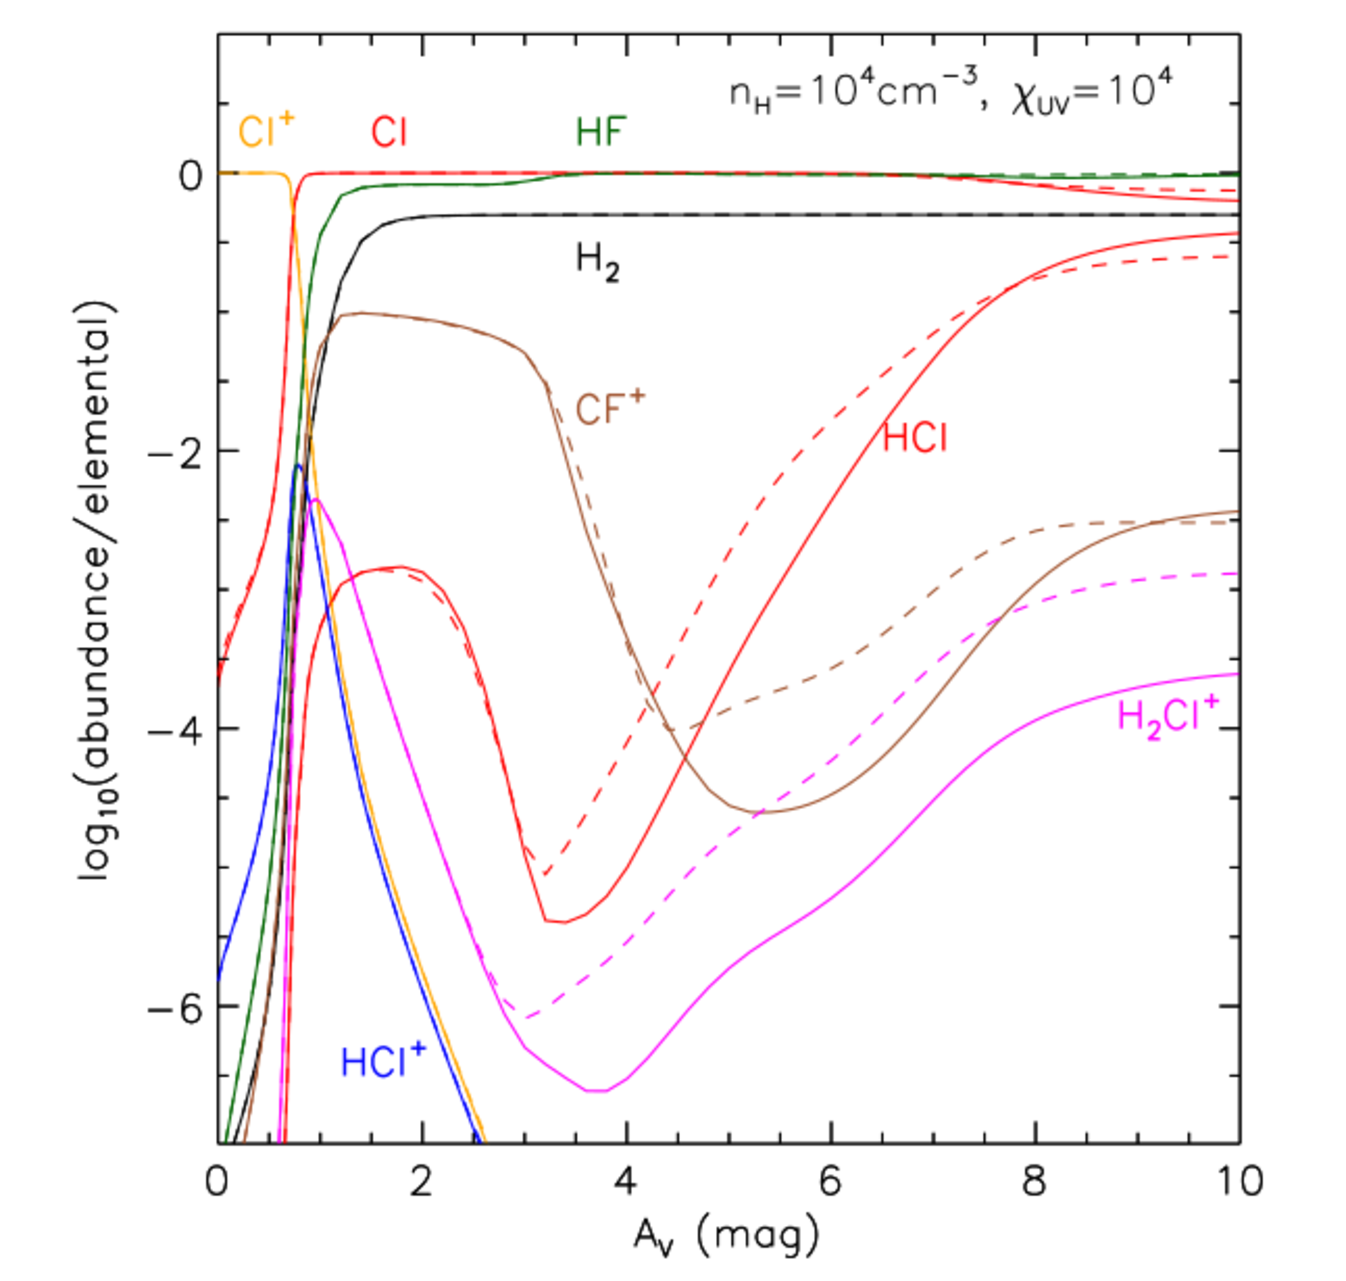
\includegraphics[trim = {0 0 0 0cm},clip,width=1\textwidth]{figure/Cl/neufire/dens.pdf}
        \caption{}
    \end{subfigure}
    ~ 
    \begin{subfigure}[t]{0.49\textwidth}
        \centering 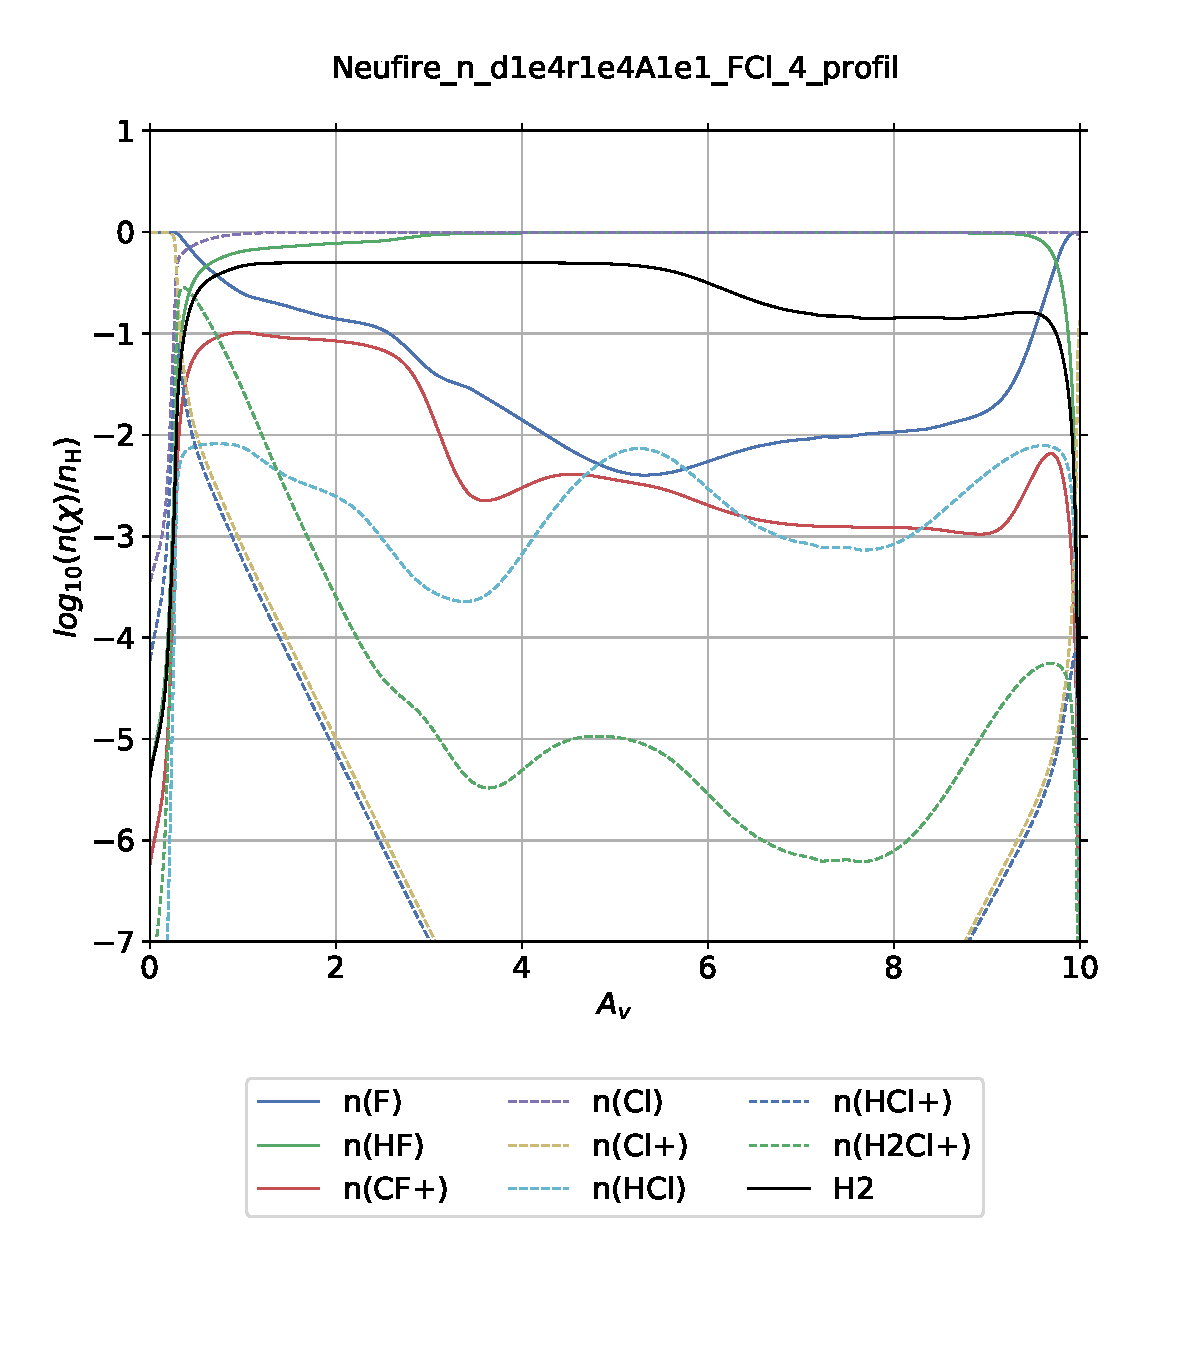
\includegraphics[trim = {0 2cm 0 1.8cm},clip,width=1\textwidth]{figure/Cl/neufire/HCl_profil.pdf}
        \caption{}
    \end{subfigure}
    
    \caption{Profil de densité pour un modèle isochore $n_\mathrm{H} = 10^4 \mathrm{cm}^{-3}$ et $\chi_\mathrm{UV} = 10^4$. La figure de gauche (a) est extraite de \cite{Neufire2009} où les profils sont obtenus à partir d'une version modifié du code de \cite{Kaufman2006}. Le trait plein est un calcul avec un taux de ionisation par les rayons cosmiques de $1.8 \times 10^{−17 } \mathrm{s}^{-1}$ par atome d'hydrogène, tandis qu'en pointillé $1.8 \times 10^{−16} \mathrm{s}^{-1}$ . A droite (b) le code PDR de Meudon résout la PDR en utilisant le même réseau chimique proposé dans l'article.}
    \label{fig:Cl:neufire}
\end{figure}

On n'arrivait pas à avoir le même profil de température, on a alors imposé au code de suivre le profil de température montré dans l'article. On utilise un modèle à densité constante qui, dans cette version du code (\uncinq), ne peut former de $\mathrm{H}_2$ dans le nuage moléculaire. Pour parer cela, on a utilisé une réaction équivalente. On voit que l'on retrouve les allures des profils de densités. Les profils du $\mathrm{Cl}$,$\mathrm{Cl}^+$, $\mathrm{HCl}$, $\mathrm{HF}$ sont proches en ordre de grandeurs. Ceux du $\mathrm{H}_2\mathrm{HF}^+$, $\mathrm{HCl}^+$, $\mathrm{CF}^+$ n'ont pas exactement les mêmes allures ni les mêmes valeurs. 

\subsubsection{radm et ladm}

\subsubsection{run sur d'autres modèles}

En runnant le code (comportant du chlore) sur d'autres types de PDR, on peut obtenir deux branches solutions possibles de températures (\ref{fig:Cl:neufire:profil}). Sur les figures, ajouter du chlore augmente subitement la température en entrée du nuage moléculaire de plus de $3000K$. Cette monté subite signifie qu'il existe probablement deux solutions stables et que le code, en résolvant la PDR, a switché de branche. Il faut aller étudier les fonctions de chauffages et de refroidissements en bord de nuage pour s'en convaincre. L'existence de deux solutions stable signifie que le gaz en bord atomique de nuage peut se trouver dans en situation de bistabilité thermique qui est un phénomène nouveau.  


\begin{figure}[htbp]
    \centering
    \begin{subfigure}[t]{0.49\textwidth} 
        \centering 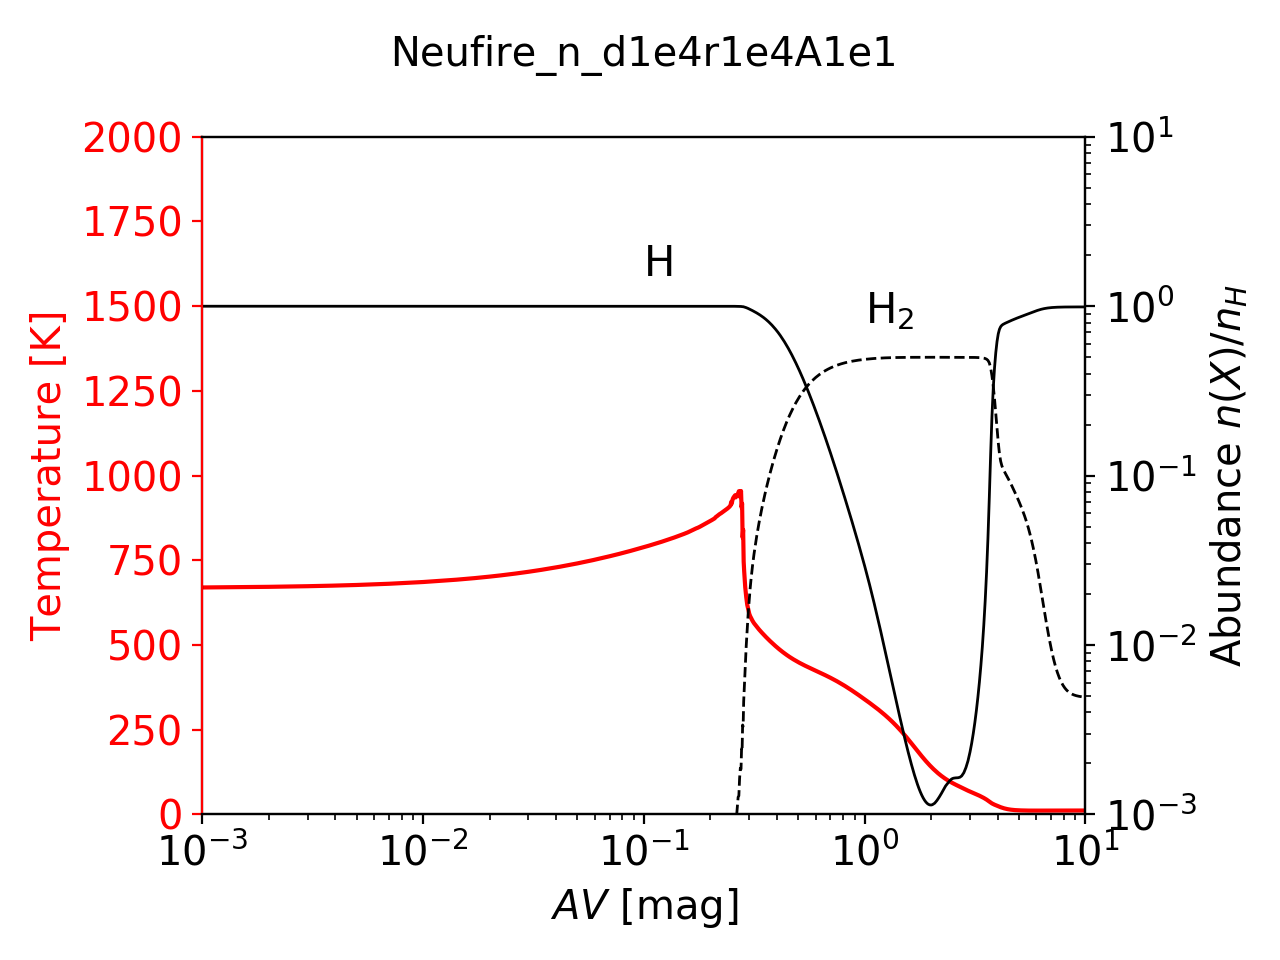
\includegraphics[trim = {0 0 0 1cm},clip,width=1\textwidth]{figure/Cl/neufire/profil_H_noCl.png}
        \caption{Sans chlore}
    \end{subfigure}
    ~ 
    \begin{subfigure}[t]{0.49\textwidth}
        \centering 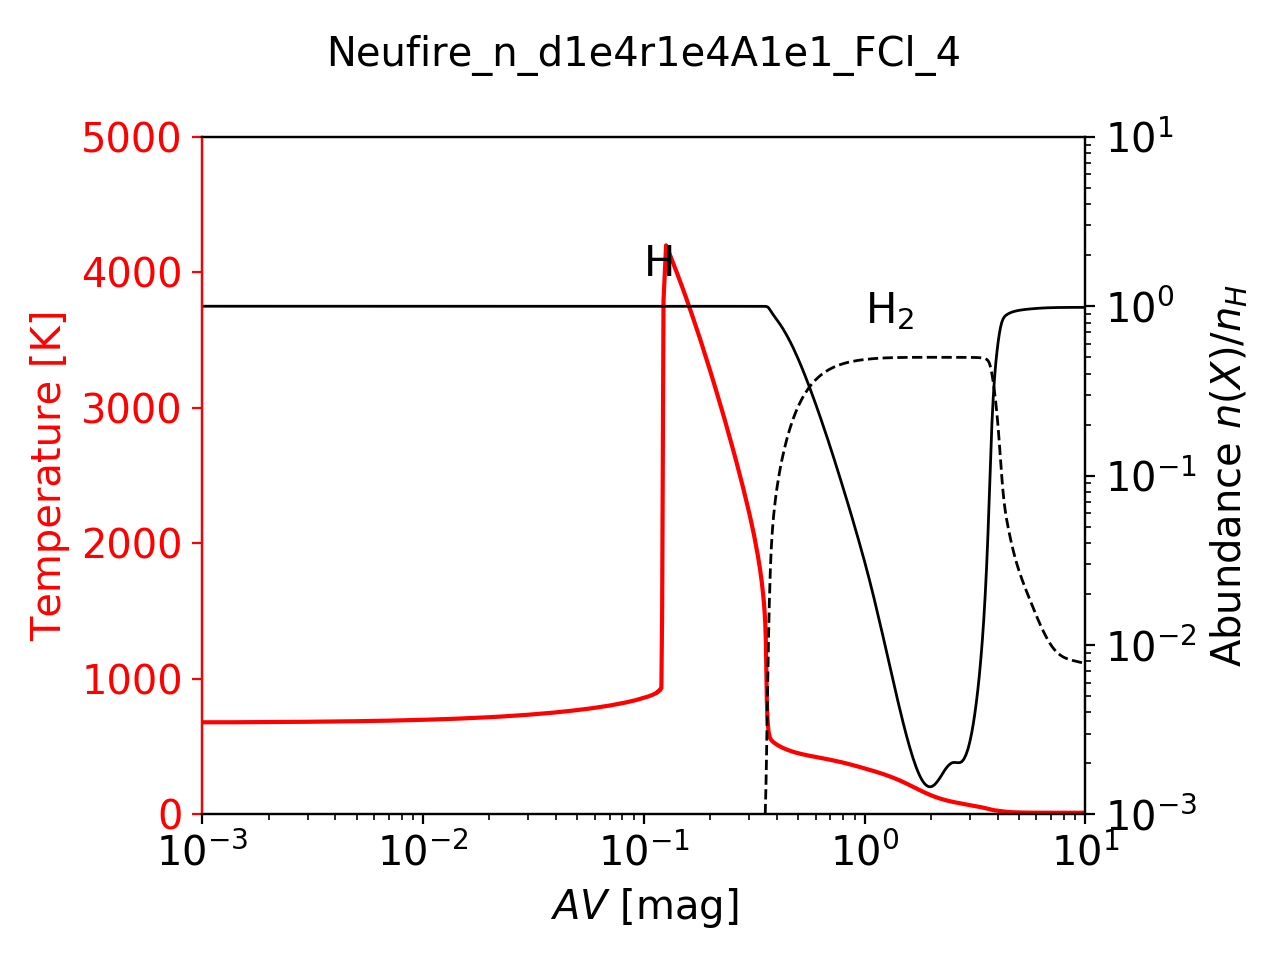
\includegraphics[trim = {0 0cm 0 1cm},clip,width=1\textwidth]{figure/Cl/neufire/profil_H.png}
        \caption{Avec chlore}
    \end{subfigure}
    \caption{}
    \label{fig:Cl:firstprofil}
\end{figure}


\subsection{Analyse du rôle du chlore}

% \begin{figure}[htbp]
%     \centering
%     \begin{subfigure}[t]{0.49\textwidth} % "0.49" donne ici la largeur de l'image
%         \centering \includegraphics[trim = {0 0 0 1cm},clip,width=1\textwidth]{figure/Cl/PDR155_n_d1e5r1e4A2e1.png}
%         \caption{Profil de température et densité en fonction de la profondeur dans le nuage}\label{fig:ClT}
%     \end{subfigure}
%     ~ 
%     \begin{subfigure}[t]{0.49\textwidth}
%         \centering \includegraphics[trim = {0 0 0 1cm},clip,width=1\textwidth]{figure/model_Cl/tb_PDR155_n_d1e5r1e4A2e1.png}
%         \caption{Taux de chauffage et refroidissement en fonction de la température du gaz au bord atomique du nuage ($A_{\mathrm{V}} = 10^{-6}$)}\label{fig:ClHC}
%     \end{subfigure}
%     \caption{Profil de densité de l'hydrogène et de la température en fonction de l'extinction dans le visible.}
% \end{figure}

J'ai étudié les réactions chimiques principales qui se déroulent en bord de nuage atomique et démontré que le chlore joue le rôle de catalyseur de l'effet photoélectrique. Le mécanisme est illustré sur la \autoref{fig:catalyseur}.
Le champs de rayonnement UV, intense en bord de nuage atomique, photoionise le chlore et produit des ions $\mathrm{Cl}^+$ et des électrons. Le transfert de charge du $\mathrm{Cl}^+$ avec l'hydrogène est une réaction rapide qui permet au chlore de se rendre de nouveau disponible pour la photoionisation. Le chlore permet ainsi de ioniser indirectement l'hydrogène. Par conséquent, la fraction électronique du gaz augmente.  
Or on sait que l'effet photoélectrique sur les grains fonctionne d'autant plus que la fraction électronique dans le nuage est importante \footnote{Une forte densité d'électrons rend plus facile la recombinaison électronique des grains ce qui maintient le degré d'ionisation des grains raisonnablement faible. Il est plus facile d'arracher un électron d'un grain neutre que d'un grain qui a déjà été ionisé.}. 
L'effet photoélectrique chauffe ainsi le gaz ce qui améliore l'efficacité du transfert de charge du $\mathrm{Cl}^+$ avec l'hydrogène. 
En d'autres termes, le chlore induit une rétroaction positive de l'effet photoélectrique sur les grains. Cet emballement a tendance à chauffer le gaz à des températures nettement plus fortes et ce malgré la faible abondance du chlore. \newline

\begin{figure}[b!]
   \centering
        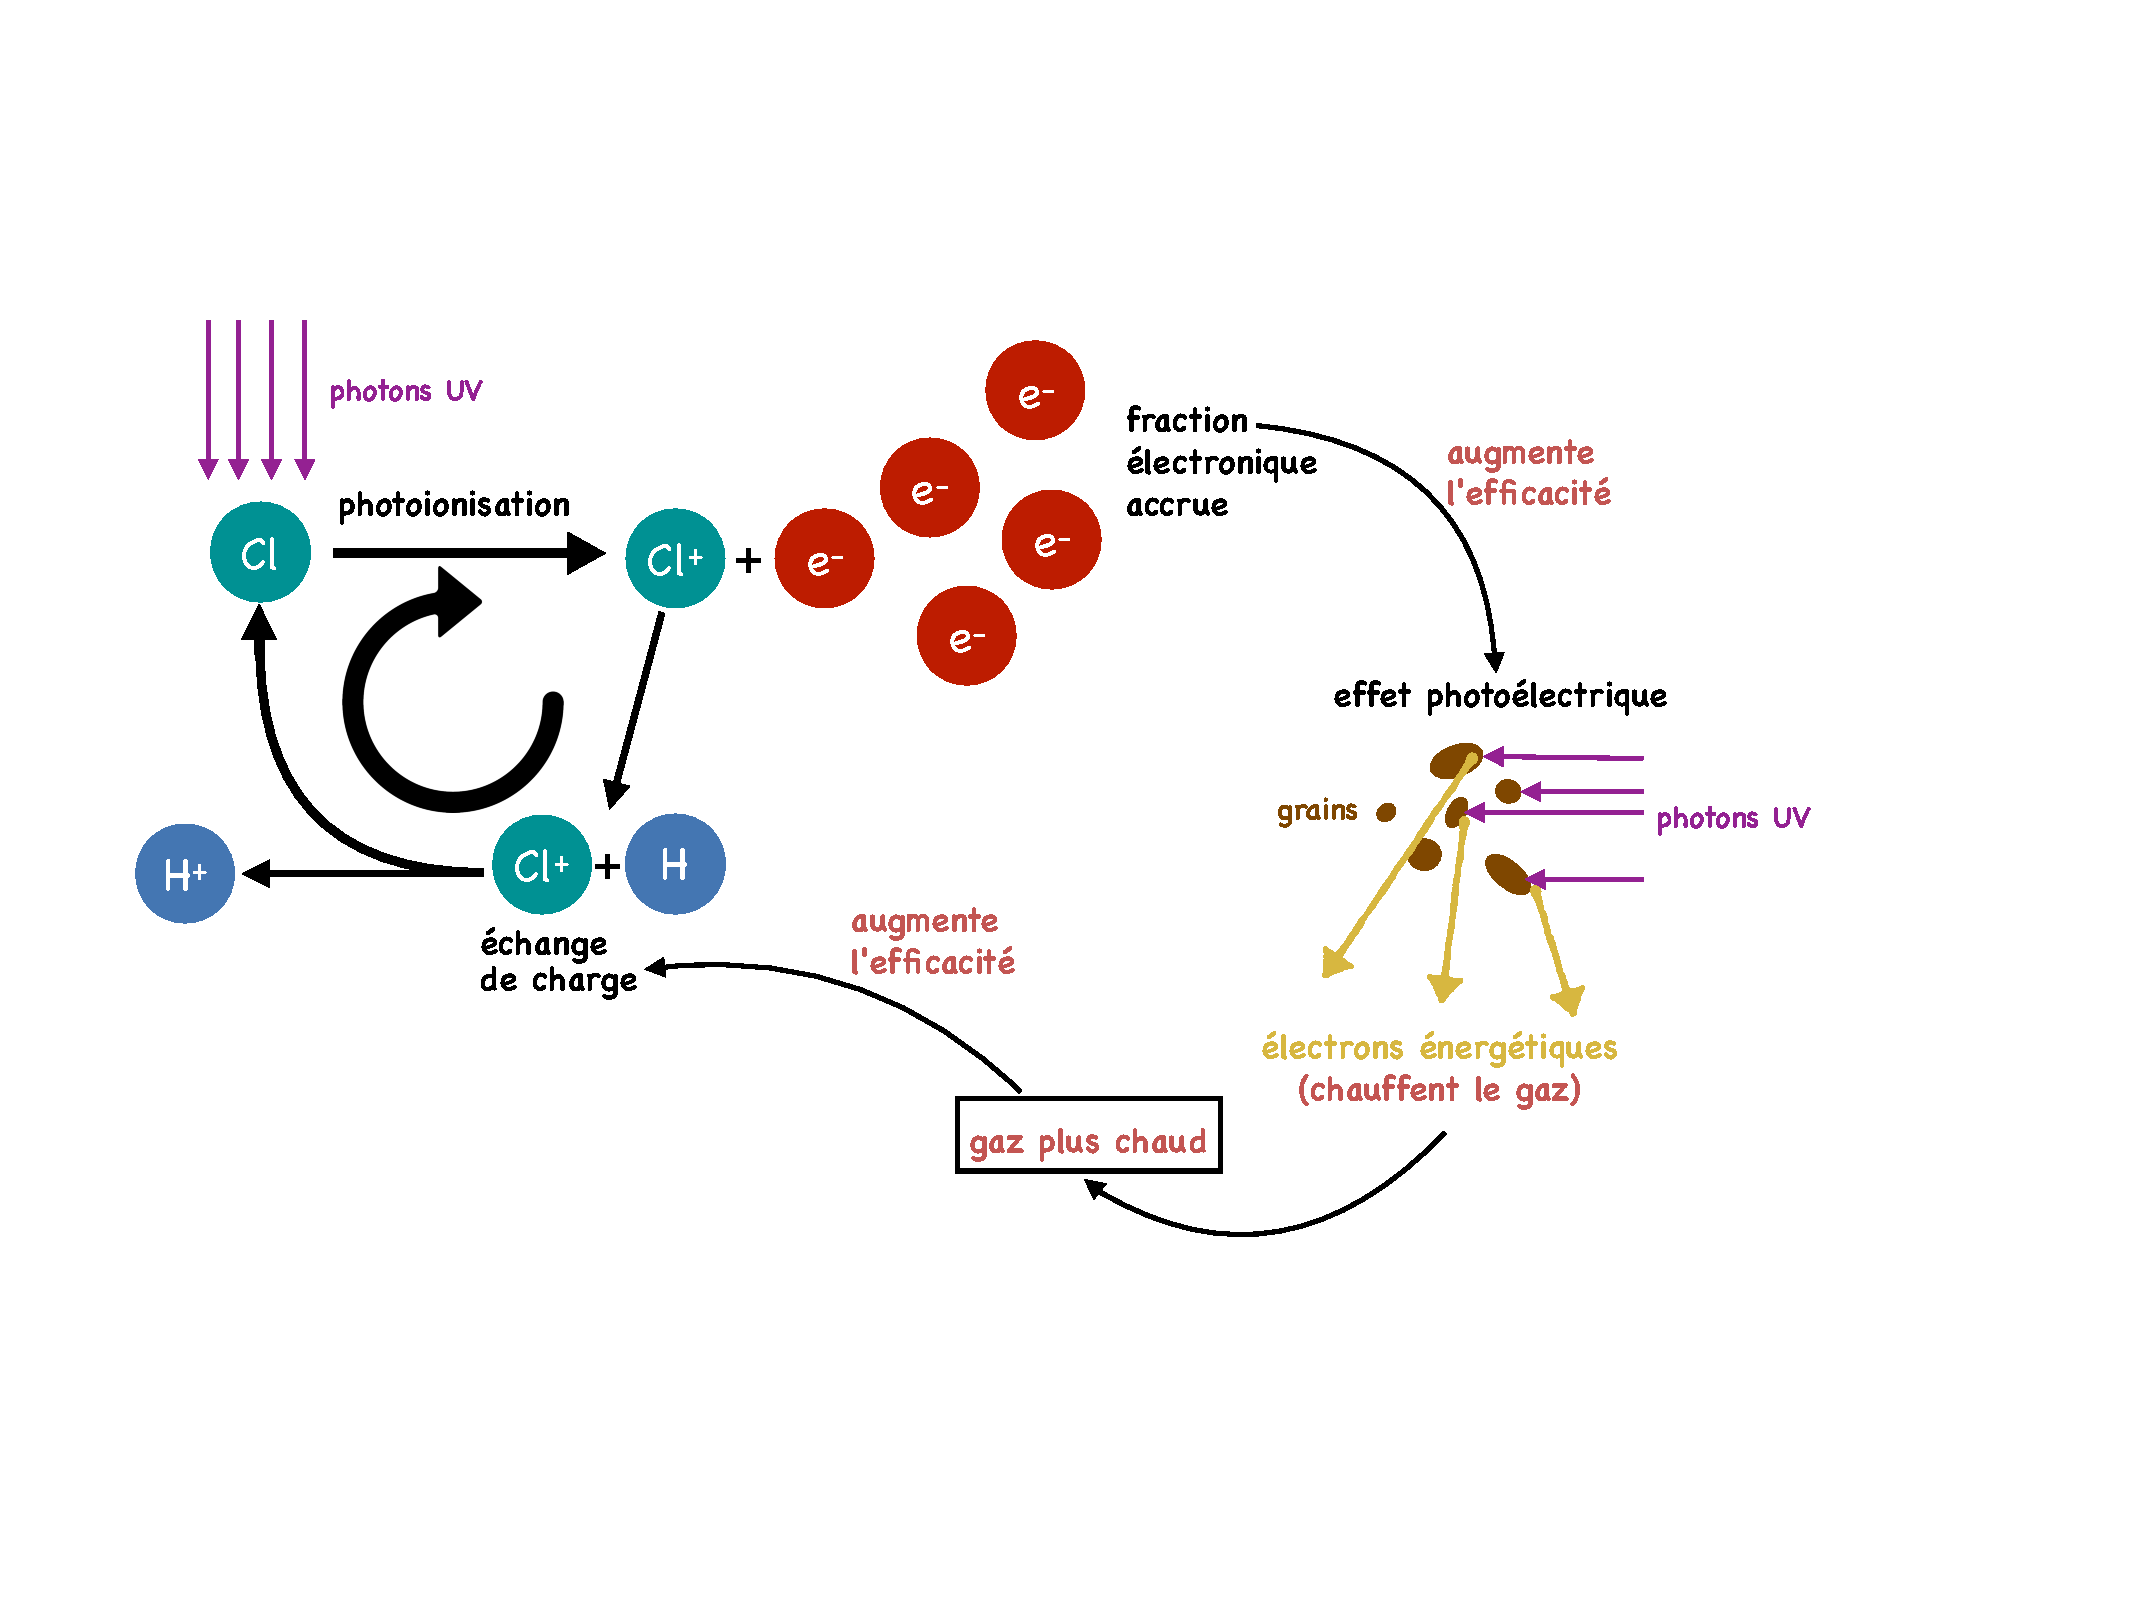
\includegraphics[trim = {2cm 5cm 4cm 4cm},clip, width=0.8\textwidth]{figure/Cl/Cl_heating_fr-5.pdf}
    \caption{Schéma représentant l'impact du chlore sur la chimie de bord de nuage atomique}
    \label{fig:catalyseur}
\end{figure}{}

L'emballement de l'effet photoélectrique se produit à partir de 1000 K. Or la photoionisation du carbone et du soufre produit les électrons en bord de nuage atomique indépendamment de la température. Il existe une température où le transfert de charge devient suffisamment efficace pour que la fraction d'électrons créée via le chlore devienne dominante devant celle de la ionisation du carbone et du soufre et amorce la rétroaction de l'effet photoélectrique. L'amplification dépend donc l'énergie d'activation du transfert de charge $\mathrm{Cl}^+  + \mathrm{H}    \rightarrow \mathrm{Cl}   +  \mathrm{H}^+$ qui vaut 6290 K. \newline

Parmi les espèces figurant dans le modèle, la carbone, le soufre, le silicium ou le fer ont également un potentiel de ionisation inférieur à celui de l'hydrogène (\autoref{tab:gaz}). Pourtant aucun ne peut effectuer un transfert de charge avec l'hydrogène qui est l'espèce majoritaire en bord de nuage atomique. Ces espèces ne peuvent pas donc pas provoquer un emballement similaire à celui induit par le chlore. 



%%%%%%%%%%%%%%%%%%%%%%%%%%%%%%%%%%%%%%%%%%%%%%%%%%%%%%%%%%%%%%%%%%%%%%%%%%%%%%%%%%%%%%%%%%%%%%%

\subsection{Modèle analytique - Chimie}

Les espèces qui contribuent à la production d'électrons en bord de nuage sont les ions hydrogènes $\mathrm{H}^+$, carbones $\mathrm{C}^+$ et soufres $\mathrm{S}^+$. On peut supposer qu'en entrée de nuage atomique le carbone et le soufre sont ionisés ce qui fournit une fraction d'électrons minimale de $10^{-4}$. Le modèle doit retrouver l'augmentation de la densité d'électrons (jusqu'à $2\ 10^{-3}$) pour des températures supérieures à 1000 K. \newline 

Le modèle que l'on propose extrapole à partir d'un modèle à densité constante fait à $n_\mathrm{H} = 10^5 \, \mathrm{cm}^{-3}$ et $\chi = 10^4$


\subsubsection{Ion hydrogène}

J'ai isolé les réactions principales qui font intervenir les ions $\mathrm{H}^+$. Les réactions avec l'oxygène sont négligées car la formation et destruction de $\mathrm{H}^+$ par l'oxygène se compensent totalement en première approximation. 

\begin{equation}
    \begin{array}{lccccclr}
        \mathrm{Cl}^+ & + &\mathrm{H}   & \rightarrow &\mathrm{Cl}  & + & \mathrm{H}^+ & (k_3) \\
        \mathrm{Cl}  & + & \mathrm{H}^+  & \rightarrow & \mathrm{Cl}^+ & + &\mathrm{H}  & (k_4) \\
        \mathrm{H}^+  & + & \mathrm{e}^-  & \rightarrow &\mathrm{H}   &   &     & (k_5) \\
    \end{array}
\end{equation}

A l'état stationnaire, le bilan de formation des ions $\mathrm{H}^+$ donne
\begin{equation}\label{eq:h+}
    \frac{d}{dt}n(\mathrm{H}^+) = k_3n(\mathrm{Cl}^+)n(\mathrm{H}) - k_4n(\mathrm{Cl})n(\mathrm{H}^+) - k_5 n(\mathrm{H}^+)n(\mathrm{e}^-) = 0
\end{equation}

En introduisant la fraction atomique de chlore $\delta_{Cl}$, fixée dans le gaz, et le bilan de charge on obtient une équation en $n(\mathrm{H}^+)$ :

\begin{equation}
    -k_3n(\mathrm{Cl}^+)n_{\mathrm{H}} + \bigg( \frac{k_3 k_4}{k_1} n_{\mathrm{H}} n(\mathrm{Cl}^+) + k_5 \big(n(\mathrm{C}^+)+ n(\mathrm{S}^+)\big) \bigg) n(\mathrm{H}^+) + k_5 n(\mathrm{H}^+)^2 = 0
\end{equation}

 avec,
\begin{equation}
    \delta_{Cl} = \SI{1.8}{10^{-7}} = \frac{n(\mathrm{Cl}) + n(\mathrm{Cl}^+) + ...}{n(\mathrm{H}) + n(\mathrm{H}^+) + 2n(\mathrm{H}_2) + ...} \approx \frac{1}{n_{\mathrm{H}}} (n(\mathrm{Cl}) + n(\mathrm{Cl}^+) )
\end{equation}

On obtient une solution qui dépend de $n(\mathrm{Cl}^+)$,
\begin{equation}
\resizebox{1.1\hsize}{!}{
    \boxed{n(\mathrm{H}^+) = -\frac{1}{2} \bigg( \frac{k_3 k_4}{k_1 k_5} n_{\mathrm{H}} n(\mathrm{Cl}^+) + n(\mathrm{C}^+)+ n(\mathrm{S}^+) \bigg) \pm \frac{1}{2} \sqrt{\bigg( \frac{k_3 k_4}{k_1 k_5} n_{\mathrm{H}} n(\mathrm{Cl}^+) + n(\mathrm{C}^+)+ n(\mathrm{S}^+) \bigg)^2 + 4\frac{k_3}{k_5}n_{\mathrm{H}} n(\mathrm{Cl}^+)}}
    }
\end{equation}

% \subsubsection{Rôle de l'oxygène}
% Au vu des taux de réactions impliquant le $\mathrm{H}^+$ nous pourrions choisir d'inclure la chimie de $\mathrm{H}^+$ avec l'oxygène. A hautes températures, les taux de $ \mathrm{H}^+ + O \leftrightarrows\mathrm{H}+ O^+ \quad (k_6,k_7)$ prédominent sur les autres réactions. Si l'on considère que ces réactions pour la chimie de l'oxygène, les $\mathrm{H}^+$ produits seront consommés pour former du $H$. Rien ne se passe. Pour s'en convaincre il suffit d'écrire la nouvelle équation bilan de $\mathrm{H}^+$ et d'utiliser celle pour $O^+$.

% \begin{equation}
%     \frac{d}{dt}n(O^+) = k_6 n(\mathrm{H}^+)n(O) - k_7n(\mathrm{H})n(O^+) = 0
% \end{equation}

% En l'injectant dans le nouveau bilan de formation pour le $\mathrm{H}^+$, ces nouveaux termes disparaissent. Cependant si l'on calcule l'expression de $n(\mathrm{H}^+)$ à partir des concentrations de $n(O^+)$ et $n(O)$, l'approximation donne une meilleure correspondance avec l'abondance calculé par le code. 

% \begin{equation}
%     n(\mathrm{H}^+) =  \frac{k_3 n_{\mathrm{H}} n(\mathrm{Cl}^+) + k_6 n_{\mathrm{H}} n(O^+) }{k_5 n(\mathrm{e}^-) + k_4 \frac{n(\mathrm{Cl}^+)}{A} + k_7 n(O) }
% \end{equation}

% Utiliser les abondances de l'oxygène demande d'étudier sa chimie, et donc de prendre en compte d'autres espèces comme $OH$ ou $O_2$ ce qui complexifie le modèle. 

%%%%%%%%%%%%%%%%%%%%%%%%%%%%%%%%%%%%%%%%%%%%%%%%%%%%%%%%%%%%%%%%%%%%%%%%%%%%%%%%%%%%%%%%%%%%%%

\subsubsection{Ion chlore}

La recombinaison électronique de $\mathrm{Cl}^+$ reste négligeable devant le transfert de charge avec $\mathrm{H}$ pour des températures supérieure à $100$K et la destruction par formation du $\mathrm{HCl}^+$ devient dominante dans la gamme de température $100-1000$K. Négliger ces réactions donne une approximation correcte de la densité d'ion chlore pour les régimes de températures $T\geq 1000$ K et garde l'emballement de l'effet photoélectrique. On considère ainsi les réactions ci-dessus :


\begin{equation}
    \begin{array}{lccccclr}
       \mathrm{Cl}  & + & h\nu & \rightarrow & \mathrm{Cl}^+ & + & \mathrm{e}^- & (k_1) \\
        \mathrm{Cl}^+ & + &\mathrm{H}   & \rightarrow &\mathrm{Cl}  & + & \mathrm{H}^+ & (k_3) \\
    \end{array}
\end{equation}

Un travail similaire nous donne 
\begin{equation}
    k_1(\xi_{Cl}n_{\mathrm{H}} - n(\mathrm{Cl}^+)) - k_3 n(\mathrm{Cl}^+) n_{\mathrm{H}} = 0
\end{equation}

Ce qui fait en posant $A = \frac{k_1}{k_3 n_{\mathrm{H}}}$:

\begin{equation}
\boxed{n(\mathrm{Cl}^+) = \frac{k_1 \xi_{Cl} n_{\mathrm{H}}}{k_1 + k_3 n_{\mathrm{H}}} = \frac{A}{1 + A} \xi_{cl} n_{\mathrm{H}}}
\end{equation}


%%%%%%%%%%%%%%%%%%%%%%%%%%%%%%%%%%%%%%%%%%%%%%%%%%%%%%%%%%%%%%%%%%%%%%%%%%%%%%%%%%%%%%%%%%%%%%%

\subsubsection{Recombinaison de $\mathrm{H}^+$ sur les grains}

La recombinaison du $\mathrm{H}^+$ sur les grains est calculé dans le code à sa manière (type 14). Le modèle chimique sans la recombinaison surestime la densité de protons aux hautes températures. \cite{Weingartner_2001} donne un taux de recombinaison $\alpha$ (équations [5][8]). 

\begin{equation}
    \alpha_{g}\left(\mathrm{X}^{i}, \psi, T\right) \approx \frac{10^{-14} C_{0} }{1+C_{1} \psi^{C_{2}}\left(1+C_{3} T^{C_{4}} \psi^{-C_{5}-C_{6} \ln T}\right)} \quad \mathrm{cm}^{3} \mathrm{s}^{-1}
\end{equation}

avec $\psi = \frac{G_0 \sqrt{T}}{n_e}$. Les coefficients $\mathrm{C}_i$ sont des paramètres donnés dans l'article. Le bilan de formation devient : 

\begin{equation}\label{eq:h+}
    \frac{d}{dt}n(\mathrm{H}^+) = k_3n(\mathrm{Cl}^+)n(\mathrm{H}) - k_4n(\mathrm{Cl})n(\mathrm{H}^+) - k_5 n(\mathrm{H}^+)n(\mathrm{e}^-) -\alpha_{g} n(\mathrm{H}^+)n_{\mathrm{H}} = 0
\end{equation}

On obtient une équation implicite en fonction de la densité d'électrons. La solution $n_e$ vérifie :
\begin{equation}
    x = n(\mathrm{H}^+)(x) + n(\mathrm{S}^+)  + n(\mathrm{C}^+)
\end{equation}

La fonction \texttt{newton} de la librairie \texttt{scipy.optimize} vient à bout de ce système. La densité d'électrons calculée montré sur la figure \ref{fig:Cl:model:rec}. On a résolu le système dans deux cas. Un cas avec les PAH (fraction massique = $4.6\,10^{-2}$) où le taux de recombinaison donné \cite{Weingartner_2001} donne une bonne estimation de la densité d'électrons. Un second cas sans PAH, où il faut réduire d'un facteur $1/6$ la recombinaison de $\mathrm{H}^+$ sur les grains. On avait toujours $r_{\mathrm{min}} = 1\,10^{-7}\,\mathrm{m}$ et $r_{\mathrm{max}} = 3\,10^{-5}\,\mathrm{m}$.

\textit{Quel réaction réduit la densité d'électrons à très hautes températures et qui nous empêche d'avoir la tangente horizontale ?}

Conclure comme quoi on arrive à produire plein d'electrons comme dans le code


\begin{figure}[htbp]
    \centering
    \begin{subfigure}[t]{0.49\textwidth} % "0.49" donne ici la largeur de l'image
        \centering 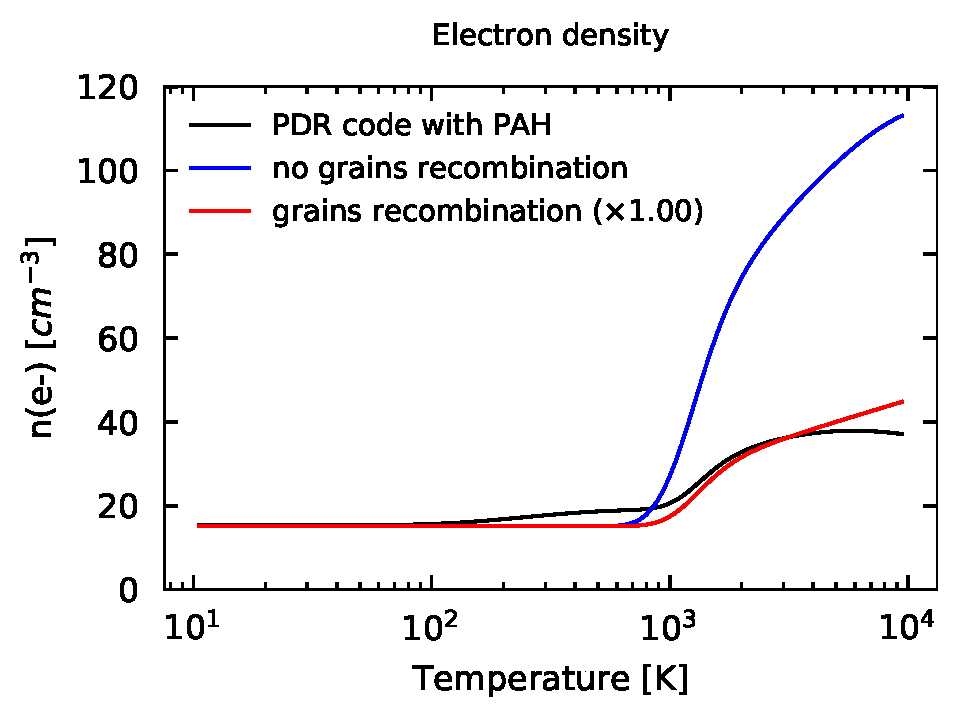
\includegraphics[trim = {0 0 0 1cm},clip,width=1\textwidth]{figure/Cl/model/test_calc_PAH_e.png}
        \caption{avec PAH}
    \end{subfigure}
    ~ 
    \begin{subfigure}[t]{0.49\textwidth}
        \centering 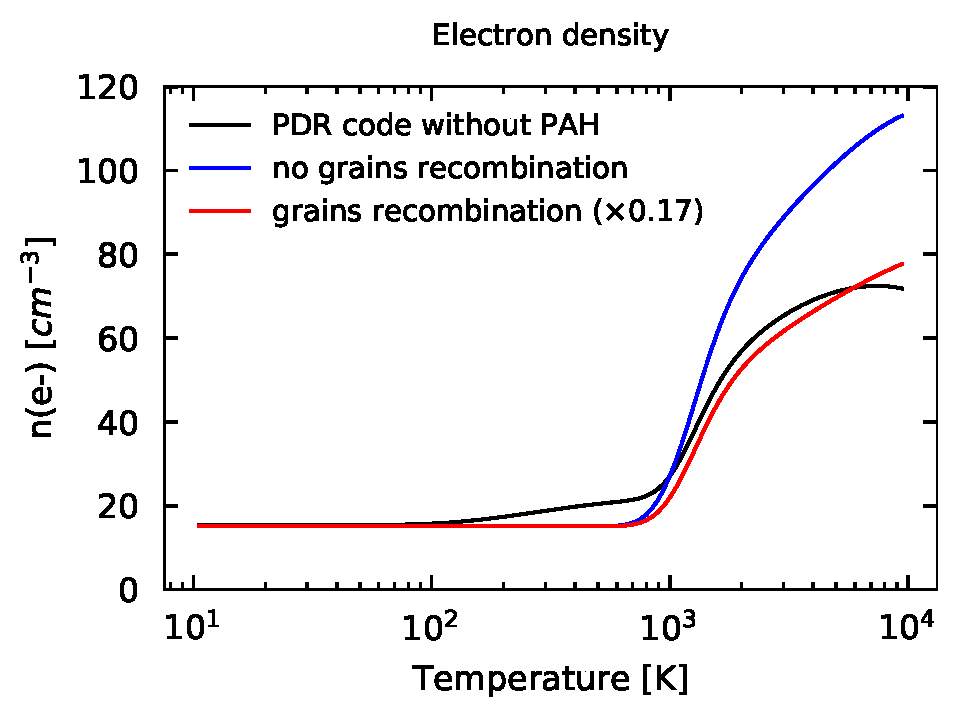
\includegraphics[trim = {0 0 0 1cm},clip,width=1\textwidth]{figure/Cl/model/test_calc_e.png}
        \caption{sans PAH}
    \end{subfigure}
    \caption{Profil de la densité électronique calculé par le modèle. La formule proposée par \cite{Weingartner_2001} prend en compte la recombinaison sur les PAH. Avec la recombinaison, la prédiction de la densité d'électrons est bonne dans le cas avec PAH. Si on ne prend pas en compte les PAH, il faut diminuer le taux de recombinaison d'un facteur $1/6$ pour prédire une densité d'électrons raisonnable.}
    \label{fig:Cl:model:rec}
\end{figure}



%%%%%%%%%%%%%%%%%%%%%%%%%%%%%%%%%%%%%%%%%%%%%%%%%%%%%%%%%%%%%%%%%%%%%%%%%%%%%%%%%%%%%%%%%%%%%%%%%%%%%%%%%%%%%%%%%%%%%%%%%%%%%%%%%%%%%%%%%%%%%%%%%%%%%%%%%%%%%%%%%%%%%%%%%%%%%%%%%%%%%%%%%%

\subsection{Modèle analytique - Thermique}

Pour construire le modèle thermique nous allons sommer l'ensemble des procesus qui interviennent en bord atomique des nuages. Par simplicité, nous négligeons le chauffage par $\mathrm{H}_2$ qui demande de connaître la densité $n(\mathrm{H}_2)$ au bord ce qui n'est pas trivial. Les processus thermiques appliqué dans le modèle sont :

\begin{itemize}
    \item l'effet photoélectrique sur les grains (\cite{BakesTielens1994})
    % \item la recombinaison électronique sur les grains
    \item le refroidissement par émission de raies de structure fine du [CII] $158 \mu m$,  [OI]$63 \mu m$, [OI]$6300A$ (\cite{Rollig2005})
    \item l'émissions Lyman $H\alpha$ (\cite{tielens2005})
    \item le couplage gaz-grain (\cite{Hollenbach1991}).
\end{itemize}{}

On dénote $\Gamma$ et $\Lambda$ les taux de chauffage et refroidissement, respectivement, total. On a 

\begin{equation}
    \begin{split}
        \Gamma &= \Gamma_{pe}^{\mathrm{Rollïg}} \\
        \Lambda &=   \Lambda_{\mathrm{CII}\ 158 \mu \mathrm{m}} + \Lambda_{\mathrm{OI}\ 63 \mu \mathrm{m}} + \Lambda_{\mathrm{OI}\ 146 \mu \mathrm{m}}  + \Lambda_{\mathrm{H}_\alpha} + \Lambda_{\mathrm{g}-\mathrm{g}} + \Lambda_{\mathrm{rec}}^{\mathrm{Rollïg}}
    \end{split}
\end{equation}


\subsubsection{Effet photoélectrique sur les grains}

De \cite{Rollig2005} (Eq (10) ou (C.3)) qui provient de \cite{BakesTielens1994}, sans PAH, on utilise : 

\begin{equation}
    \Gamma_{\mathrm{pe}} = 10^{-24}\,G_0\,n_\mathrm{H}\, \frac{2\times 10^{-2}}{1 + 2\times 10^{-4}\,G_0 \sqrt{T}/n_e} \qquad \operatorname{erg} \mathrm{cm}^{-3} \mathrm{s}^{-1}
    \label{eq:Rollig:pe}
\end{equation}

Avec $G_0 = 1.71\chi \times 0.5$ car il considère une illumination provenant que d'un coté. (\cite{Wolfire_2003} Eq 20, \cite{BakesTielens1994}) propose une autre formule prenant en compte les PAH qui est de la forme 

\begin{equation}
    \Gamma_{\mathrm{pe}}^{\mathrm{Wolf}} = 10^{-24}\,G_0\,n_\mathrm{H}\, \bbig[ \frac{4.9\times 10^{-2}}{1 + 4\times 10^{-3}\, \frac{G_0 \sqrt{T}}{n_e \phi_\mathrm{PAH}}} + \frac{3.7\times 10^{-2} (T/10^4)^{0.7}}{1 + 2\times 10^{-4}\, \frac{G_0 \sqrt{T}}{n_e \phi_\mathrm{PAH}}} \bbig]\qquad  \operatorname{erg} \mathrm{cm}^{-3} \mathrm{s}^{-1}
\end{equation}

avec $\phi_\mathrm{PAH}$ une efficacité de collision compris entre 0 et 1. L'effet photoélectrique est d'autant plus efficace sur les petits grains \cite{DraineBook}. Le choix de $r_\mathrm{min}$ (la taille minimale des grains dans la description MRN) est décisif. Si l'on trace ces formules sur la \autoref{fig:Cl:pePAH} pour différent $\phi_\mathrm{PAH}$ et $r_\mathrm{min}$ on voit que la formule de \cite{Rollig2005} sous-estime le taux calculé par le code PDR de Meudon. Avec $r_\mathrm{min} = 1\,10^7\,\mathrm{nm}$, la prescription de Rollig est 3 fois plus petit que le chauffage calculé par Meudon. Si l'on augmente la taille de grain minimale, on voit que cette écart diminue ce qui est cohérent car on enlève des petits grains. La prescription de \cite{Wolfire_2003} laisse plus de liberté à travers le $\phi_\mathrm{PAH}$ (à mieux dire).

\begin{figure}[!h]
    \centering
    \begin{subfigure}[t]{0.49\textwidth} % "0.49" donne ici la largeur de l'image
        \centering 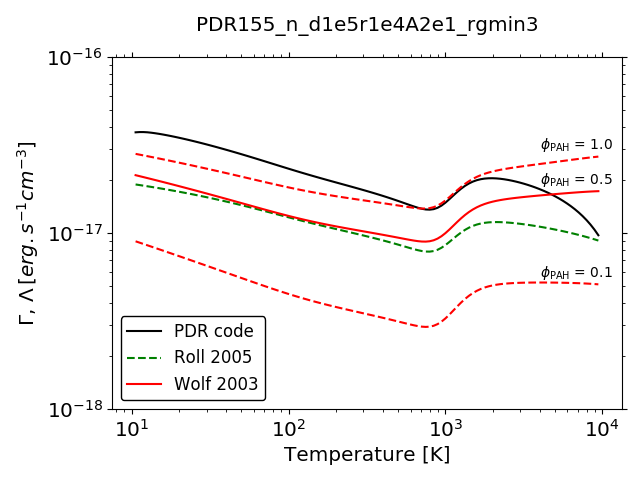
\includegraphics[trim = {0 0 0 1cm},clip,width=1\textwidth]{figure/Cl/pePAH/pe_formulae_rgmin3.png}
        \caption{$r_\mathrm{min} = 3\,10^{-7} \, \mathrm{nm}$}
    \end{subfigure}
    ~ 
   \begin{subfigure}[t]{0.49\textwidth} % "0.49" donne ici la largeur de l'image
        \centering 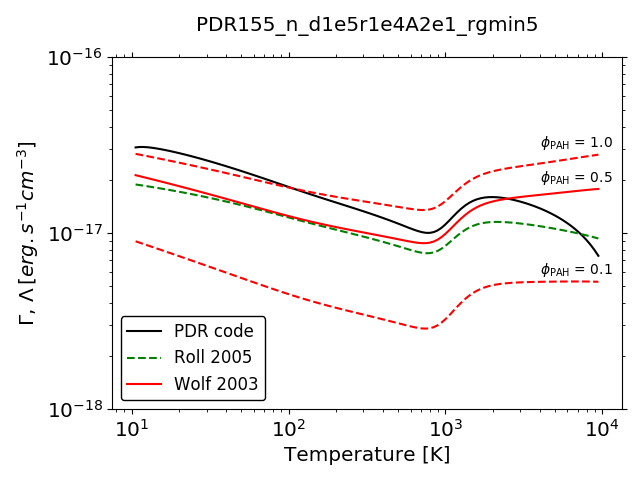
\includegraphics[trim = {0 0 0 1cm},clip,width=1\textwidth]{figure/Cl/pePAH/pe_formulae_rgmin5.png}
        \caption{$r_\mathrm{min} = 5\,10^{-7}\, \mathrm{nm}$}
    \end{subfigure}
    \caption{Comparaison des formules de l'effet photoélectrique de \cite{Rollig2005} et \cite{Wolfire_2003} avec le code PDR pour différents $r_\mathrm{min}$}
    \label{fig:Cl:pePAH}
\end{figure}

%%%%%%%%%%%%%%%%%%%%%%%%%%%%%%%%%%%%%%%%%%%%%%%%%%%%%%%%%%%%%%%%%%%%%%%%%%%%%%%%%%%%%%%%%%%%%%%

\subsubsection{Couplage gaz-grains}

De \cite{Rollig2005} ($Z=1$), le couplage gaz grain s'exprime,

\begin{equation}
    \Lambda_{\mathrm{g}-\mathrm{g}} = 3.5\,10^{-34}\times \sqrt{T}(T - T_g) {n_\mathrm{H}}^2 \qquad \operatorname{erg} \mathrm{cm}^{-3} \mathrm{s}^{-1}
\end{equation}

Où $T_g$ est donné par Eq. 6 de \cite{HollenbachTakahashiTielens_1991}
\begin{equation}
    T_g = 12.2 \,{G_0}^{0.2}
\end{equation}

%%%%%%%%%%%%%%%%%%%%%%%%%%%%%%%%%%%%%%%%%%%%%%%%%%%%%%%%%%%%%%%%%%%%%%%%%%%%%%%%%%%%%%%%%%%%%%%


\subsubsection{Refroidissement par les raies d'émissions du $\mathrm{C}^+$ et de $\mathrm{O}$}

[CII]$158 \mu \mathrm{m}$, provient de \cite{Rollig2005}, Equation (A.2) ($Z=1$)

\begin{equation}
    \Lambda_{\mathrm{CII}\ 158   \mu \mathrm{m}}= n(\mathrm{C}^+) \frac{2.89 \times 10^{-20}}{1+\frac{1}{2} \exp (92 / T)\left(1+\frac{1300}{n_\mathrm{H}}\right)} \qquad \operatorname{erg} \mathrm{cm}^{-3} \mathrm{s}^{-1}
\end{equation}

Pour les raies de [OI], Rollïg prend en compte les transitions adjacentes de [OI]$62 \mu \mathrm{m}$ et $[OI]146 \mu \mathrm{m}$. ($Z$,$\beta = 1$)


\begin{equation}
\begin{split}
    \Lambda_{\mathrm{OI}\ 63 \mu \mathrm{m}} &= 3.15\,10^{-14} \times 8.46\,10^{-5} \times 
    n(\mathrm{O}) \\
    & \times \frac{e^{98/T} 3 n_\mathrm{H} (n_\mathrm{H} + \beta\, n_{\mathrm{cr}_{01}} ) }{{n_\mathrm{H}}^2+ e^{98/T}(n_\mathrm{H} + \frac{1}{2} n_{\mathrm{cr}_{01}} ) (3 n_\mathrm{H} + 5\, e^{228/T} (n_\mathrm{H} + \frac{1}{2} n_{\mathrm{cr}_{12}} )) } \qquad \operatorname{erg} \mathrm{cm}^{-3} \mathrm{s}^{-1}
\end{split}
\end{equation}

\begin{equation}
\begin{split}
    \Lambda_{\mathrm{OI}\ 146 \mu \mathrm{m}} &= 1.35\,10^{-14} \times 8.46\,10^{-5} \times 
    n(\mathrm{O}) \\
    & \times \frac{ {n_\mathrm{H}}^2 }{n_\mathrm{H}^2+ e^{98/T}(n_\mathrm{H} + \frac{1}{2} n_{\mathrm{cr}_{01}} ) (3 n_\mathrm{H} + 5\, e^{228/T} (n_\mathrm{H} + \frac{1}{2} n_{\mathrm{cr}_{12}} )) } \qquad \operatorname{erg} \mathrm{cm}^{-3} \mathrm{s}^{-1}
\end{split}
\end{equation}

Avec $n_{\mathrm{cr}_{01}}(T) = \frac{1.66\,10^{-5} }{1.35\,10^{-11} T^{0.49}} $ et $n_{\mathrm{cr}_{12}}(T) = \frac{8.46\,10^{-5} }{4.37\,10^{-12} T^{0.66}} $

%%%%%%%%%%%%%%%%%%%%%%%%%%%%%%%%%%%%%%%%%%%%%%%%%%%%%%%%%%%%%%%%%%%%%%%%%%%%%%%%%%%%%%%%%%%%%%%

\subsubsection{Emission Lyman $\mathrm{H}\alpha$}

\cite{tielens2005}, Eq 2.62

\begin{equation}
    \Lambda_{\mathrm{H}\alpha} = 7.3\, 10^{-19}\,n_e\,n_\mathrm{H}\,e^{-118400/T} \qquad \operatorname{erg} \mathrm{cm}^{-3} \mathrm{s}^{-1}
\end{equation}

%%%%%%%%%%%%%%%%%%%%%%%%%%%%%%%%%%%%%%%%%%%%%%%%%%%%%%%%%%%%%%%%%%%%%%%%%%%%%%%%%%%%%%%%%%%%%%%

\subsubsection{Recombinaison des électrons sur les grains}

Dans le modèle de chlore, on prend celle de \cite{Rollig2005} Eq.4  qui provient elle même de \cite{BakesTielens1994}.

\begin{equation}
    \Lambda_{\mathrm{rec}}^{\mathrm{Rollïg}} = 3.49\,10^{-30} T^{0.944} \, (\frac{G_0 \sqrt{T}}{n_e})^{\frac{0.735}{T^{0.068}}} \, n_e \, n_\mathrm{H} \qquad \operatorname{erg} \mathrm{cm}^{-3} \mathrm{s}^{-1}
    \label{eq:Rollig:rece}
\end{equation}

Il existe également celle ci \cite{WolfireHollenbachMcKeeTielensBakes_1995} Eq. 9 que l'on n'utilise pas.

\begin{equation}
    \Lambda_{\mathrm{rec}}^{\mathrm{Wolfire}} = 4.65\,10^{-30} T^{0.94} \, (\frac{G_0 \sqrt{T}}{n_e})^{\frac{0.74}{T^{0.068}}} \, n_e \, n_\mathrm{H} \qquad \operatorname{erg} \mathrm{cm}^{-3} \mathrm{s}^{-1}
\end{equation}

%%%%%%%%%%%%%%%%%%%%%%%%%%%%%%%%%%%%%%%%%%%%%%%%%%%%%%%%%%%%%%%%%%%%%%%%%%%%%%%%%%%%%%%%%%%%%%%

\subsection{Correction de l'effet photoélectrique par le code}

On compare le modèle thermo-chimique que l'on a construit à un modèle à densité densité constante résolu par le code PDR afin de vérifier que l'on obtient une température d'équilibre sensiblement égale. \newline

Connaissant les expressions des termes de chauffages $\Gamma$ et $\Lambda$ et étant capable de calculer une densité d'électrons $n_e$ en fonction de la température, on détermine les températures d'équilibre $T_{\mathrm{éq}}$ définies telles que $\Gamma - \Lambda  = 0$. Un point d'équilibre est stable (instable) si autour de $T_{eq}$, $\frac{d}{dT}(\Gamma - \Lambda)$ est négatif (positif). \newline 

On trace les sur la figure \ref{fig:Cl:modelPE:GC} les courbes de chauffage et de refroidissement au bord de nuage pour un modèle $n_\mathrm{H} = 10^{4.5} \,\mathrm{cm}^{-3}$ et $\chi = 10^4$. On remarque que notre modèle retrouve bien l'emballement de l'effet photo-électrique à partir de $1000$ K. Par ailleurs, on constate que le calcul de Rollïg (eq \ref{eq:Rollig:pe} sous estime d'un facteur d'environ 3 l'effet photo-électrique calculé par le code. La solution chaude calculé par le modèle est $4000$ K plus froide que celle obtenue par le code et est similaire à la température obtenue par un modèle ne comportant pas de chlore. Afin de pouvoir différencier les modèles qui sont impacté par l'instabilité par le chlore de ceux qui ne le sont pas, on corrige la formule de l'effet photoélectrique de Rollïg d'un facteur 3. La température d'équilibre que l'on obtient alors est proche de la solution chaude obtenue par le code PDR ($+1500$ K). Dans la suite, le modèle utilisera toujours comme expression du chauffage par effet photoélectrique celle de Rollïg multiplié d'un facteur 3. 


\begin{figure}[!h]
    \centering
    \begin{subfigure}[t]{0.49\textwidth} % "0.49" donne ici la largeur de l'image
        \centering 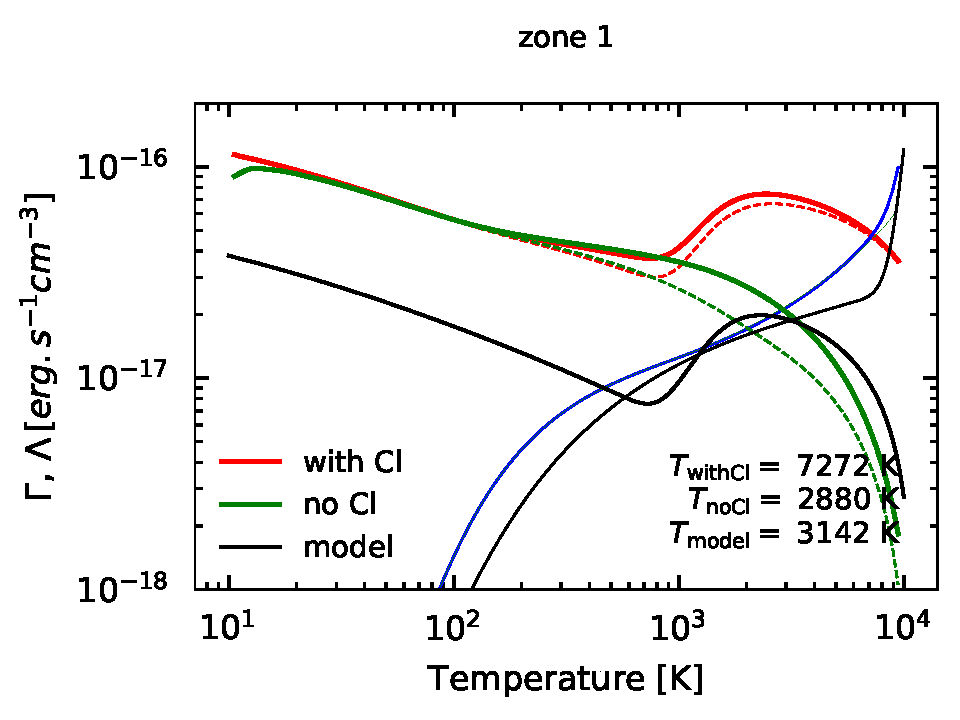
\includegraphics[trim = {0 0 0 2 },clip,width=1\textwidth]{figure/Cl/modelPE/GCcomp_Cl_1_1.pdf}
        \caption{$\Gamma =  \Gamma_{pe}^{\mathrm{Rollïg}}$}
    \end{subfigure}
    ~ 
    \begin{subfigure}[t]{0.49\textwidth}
        \centering 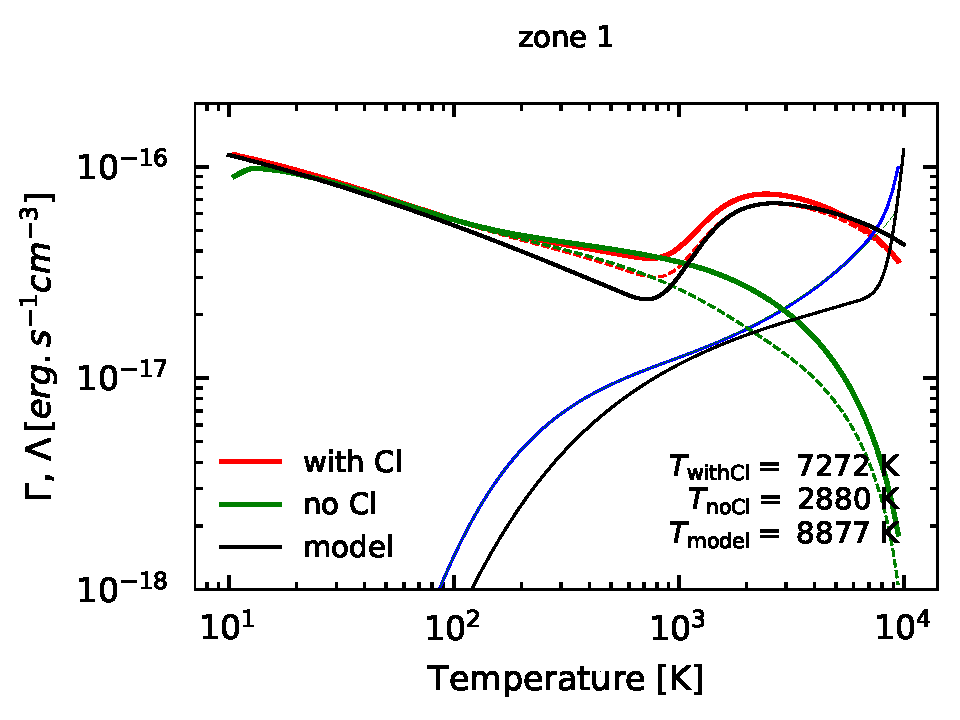
\includegraphics[trim = {0 0 0 2 },clip,width=1\textwidth]{figure/Cl/modelPE/GCcomp_Cl_1_3.pdf}
        \caption{$\Gamma =  3 \times \Gamma_{pe}^{\mathrm{Rollïg}}$}
    \end{subfigure}
    \caption{Courbes de chauffage et refroidissement au bord atomique d'un modèle à densité constante ($n_\mathrm{H} = 10^{4.5} \,\mathrm{cm}^{-3}$ et $\chi = 10^4$). Le trait en pointillé rouge et vert représente l'effet photoélectrique pour les modèles comportant ou non du chlore.  Le trait plein est le chauffage total. Dans ces conditions physique, le chauffage par la molécule $\mathrm{H}_2$, qui n'est pas pris en compte dans le modèle, est moins intense que l'effet photoélectrique. Les courbes de refroidissements sont en bleues et quasi-identiques selon qu'il y ait du chlore ou non. La courbe en trait noir est le terme de chauffage du modèle, l'effet photoélectrique sur les grains, calculé grace à la formule de Rolllig. La courbe de refroidissement du modèle est en trait fin noir.}
    \label{fig:Cl:modelPE:GC}
\end{figure}

\subsection{Prédiction de la température au bord de nuage}
 
A l'aide de ce modèle nous pouvons chercher dans quelles conditions ($n\mathrm{H}$ et $\chi$) les bords atomiques des PDR vivent l'instabilité provoqué par le chlore. Pour étudier globalement les PDR, on utilise des grilles de modèles qui varient dans l'espace des paramètres (densité $n_\mathrm{H}$ et le champ de rayonnement de l'étoile proche $\chi$). Le code PDR résout chaque modèle puis l'on représente une donnée - la température au bord de nuage ou le processus thermique dominant au bord du nuage - dans l'espace des paramètres. On préfère étudier des modèles à densités constantes qui sont plus facile à interpréter (la pression et la température suivent les mêmes variations $\mathrm{P}\propto \mathrm{T}$) que les modèles isobares (la densité et la température varient de manière inversement proportionelle $\mathrm{n}_\mathrm{H}\mathrm{T}=\mathrm{cte}$). 


\subsubsection{Carte de température au bord du nuage}

La figure \ref{fig:Cl:gridModel:Tba} représente la température d'équilibre maximale calculée par notre modèle. On constate que les bords atomiques des régions fortement illuminées augmentent chauffent de plusieurs milliers de Kelvin en présence de chlore le nuage. 
Il apparaît également des instabilités thermiques dans les régions diffuses et fortement illuminées ($n_\mathrm{H} \leq 10^4 \, \mathrm{cm}^{-3}$ et $\chi \geq 10^2$) . \newline 


\begin{figure}[!h]
    \centering
    \begin{subfigure}[t]{0.49\textwidth} % "0.49" donne ici la largeur de l'image
        \centering 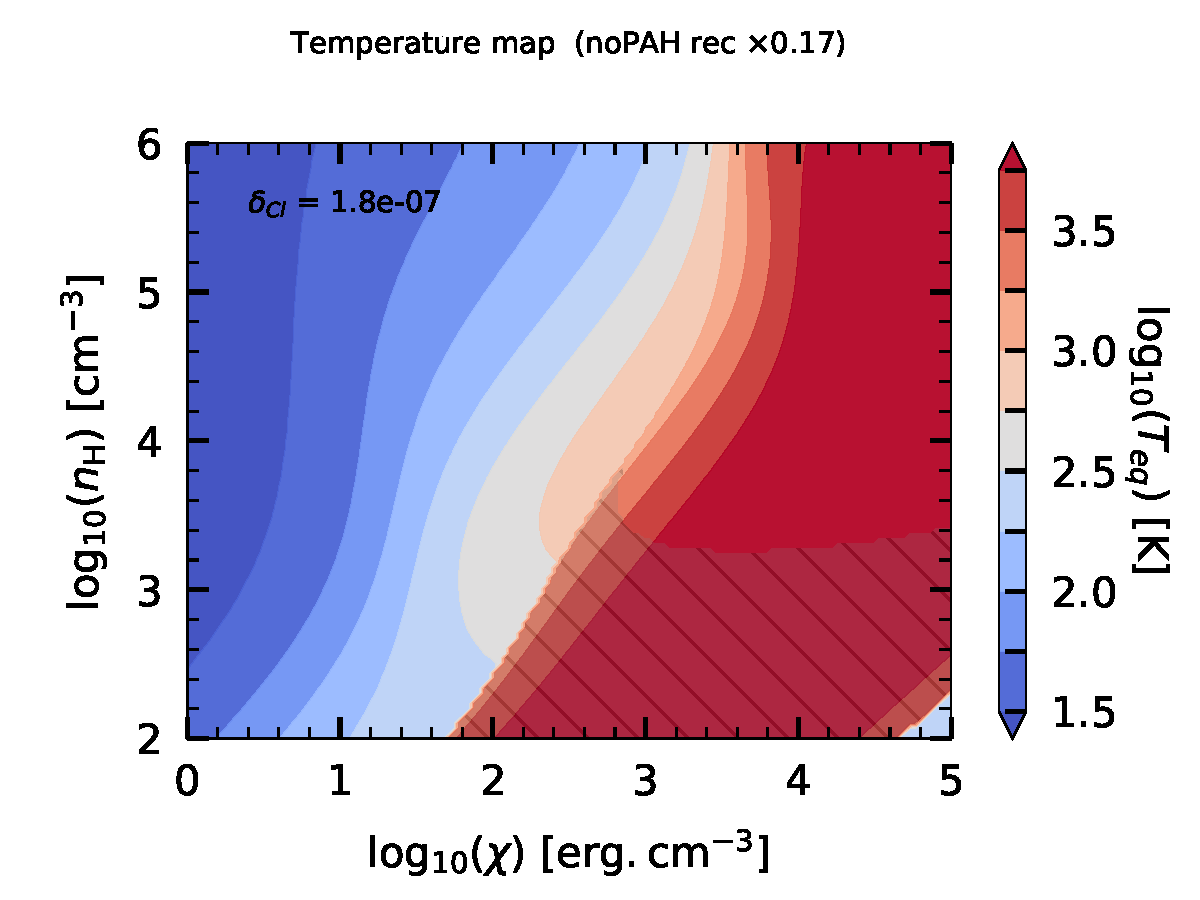
\includegraphics[trim = {0 0 0 1cm},clip,width=1\textwidth]{figure/Cl/gridModel/mapG0nHTeq_m6p7_imp_noPAH_3p0PE_OI_CII_ggr_elecrec_lyman_OI.pdf}
        \caption{avec chlore}
    \end{subfigure}
    ~ 
    \begin{subfigure}[t]{0.49\textwidth}
        \centering 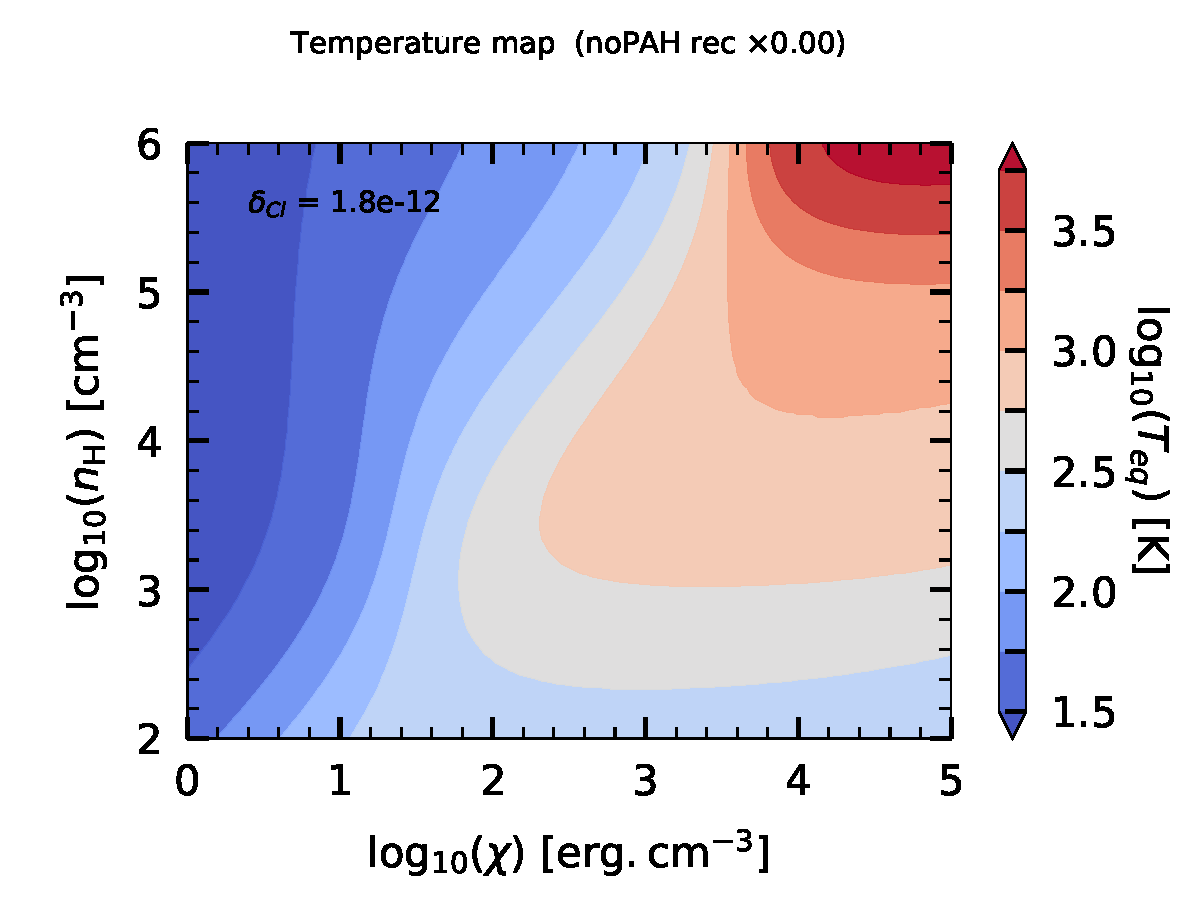
\includegraphics[trim = {0 0 0 1cm},clip,width=1\textwidth]{figure/Cl/gridModel/mapG0nHTeq_m11p7_exp_noPAH_3p0PE_OI_CII_ggr_elecrec_lyman_OI.pdf}
        \caption{sans chlore}
    \end{subfigure}
    \caption{Carte de température prédite par le modèle}
     \begin{minipage}{\textwidth} 
     La zone hachurés sur la figure (a) signifie qu'il existe également une solution instable.
     \label{fig:Cl:gridModel:Tba:noCl}
     \end{minipage}
    \label{fig:Cl:gridModel:Tba}
\end{figure}


% différence de lorsque l'on ajoute du chlore ou non
Les cartes de température calculés grâce au code PDR (figure \ref{fig:Cl:grid:Tba}) réduisent la zone concernée par l'emballement du chauffage, induit par le chlore, seulement aux régions denses et fortement illuminées ($n_\mathrm{H} \geq 10^4 \, \mathrm{cm}^{-3}$ et $\chi \geq 10^3$).  \newline 

Néanmoins, on ne parvient pas à retrouver les températures annoncées par le modèle dans les régions moins denses. Cette différence est causée, dans une certaine mesure, par la formule de l'effet photoélectrique qui a été choisi et de la méthode de résolution du code PDR. 

Sur la figure \ref{fig:Cl:grid:Tba:noCl} on remarque l'existence d'un point-selle en température vers $n_\mathrm{H}=10^3 \, \mathrm{cm}^{-3}$ et $\chi=10^3$ qu'y est absent sur la figure \ref{fig:Cl:gridModel:Tba:noCl}. Une analyse de cette région montre, que d'après le code dans les régions à basse densité, si l'on augmente l'intensité du champs de rayonnement $\chi$ alors la recombinaison des électrons sur les grains devient progressivement plus efficace que l'effet photoélectrique pur ce qui refroidit le gaz. Les formules de l'effet photoélectrique (eq \ref{eq:Rollig:pe}) et de la recombinaisons des électrons sur les grains (eq \ref{eq:Rollig:rece}) que l'on a choisit reproduisent mal ce phénomène. Le gaz, dans le modèle, est alors plus chaud. <discussion sur la remonté quand nh diminue>. 

Pour trouver la température d'équilibre, le code PDR de Meudon cherche le zéros de la fonction $\mathrm{T} \rightarrow (\Gamma - \Lambda)(\mathrm{T)}$ par dichotomie. Il obtiendra, dans le cas d'une bistabilité, une des solutions stables sans savoir laquelle est la plus chaude. En effet, sur la figure \ref{fig:Cl:particulier:2}, le code de Meudon trouve la solution basse température alors qu'il existait une solution chaude proche de $9000$ K. Une amélioration que pourrait subir le code est de le rendre capable de déceler deux solutions (s'il y en a) et de rester sur une même branche de solution à travers le nuage. Cela permettrait de ne plus avoir des profils de température tel que celui de la figure \ref{fig:Cl:firstprofil}. \newline 

\begin{figure}[!h]
    \centering
    \begin{subfigure}[t]{0.49\textwidth} % "0.49" donne ici la largeur de l'image
        \centering 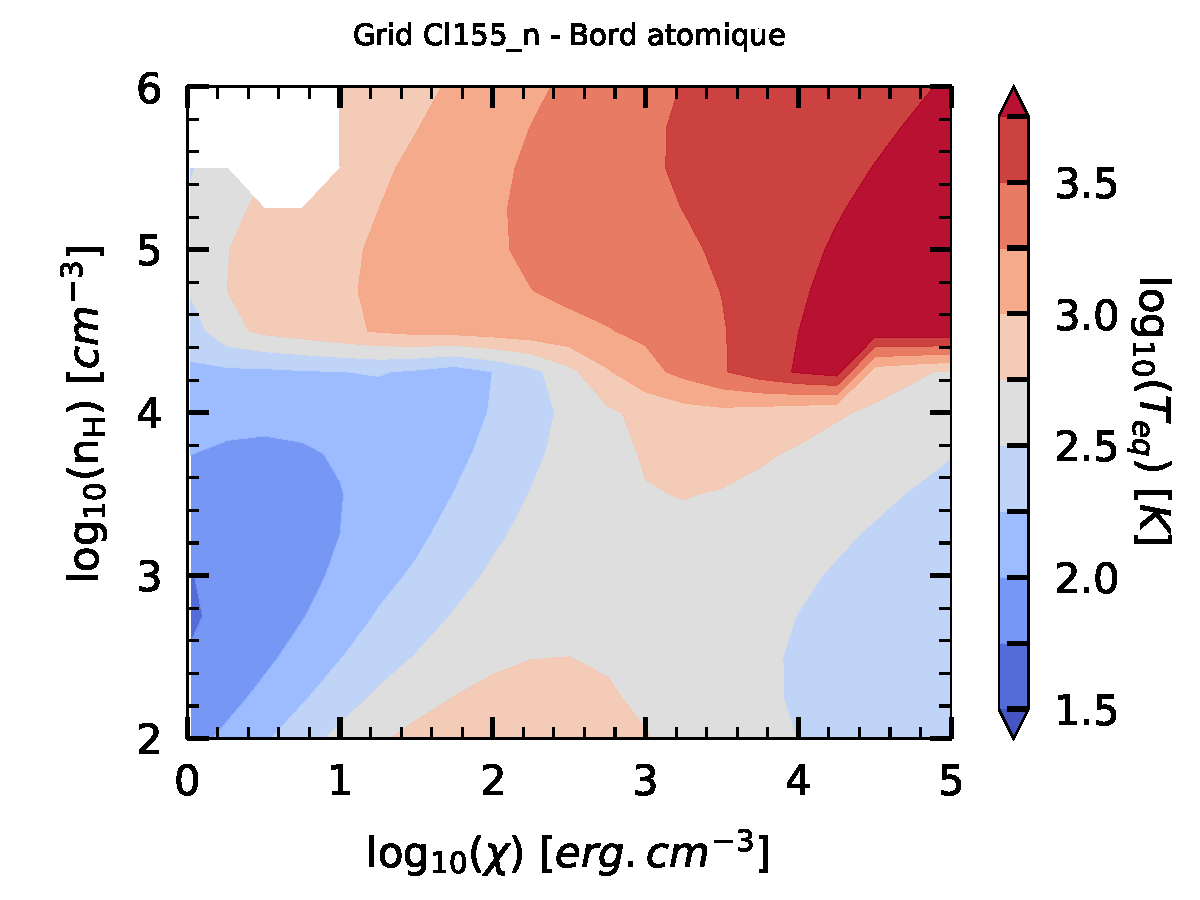
\includegraphics[trim = {0 0 0 1cm},clip,width=1\textwidth]{figure/Cl/gridCl155_n/mapTba.pdf}
        \caption{avec chlore}
    \end{subfigure}
    ~ 
    \begin{subfigure}[t]{0.49\textwidth}
        \centering 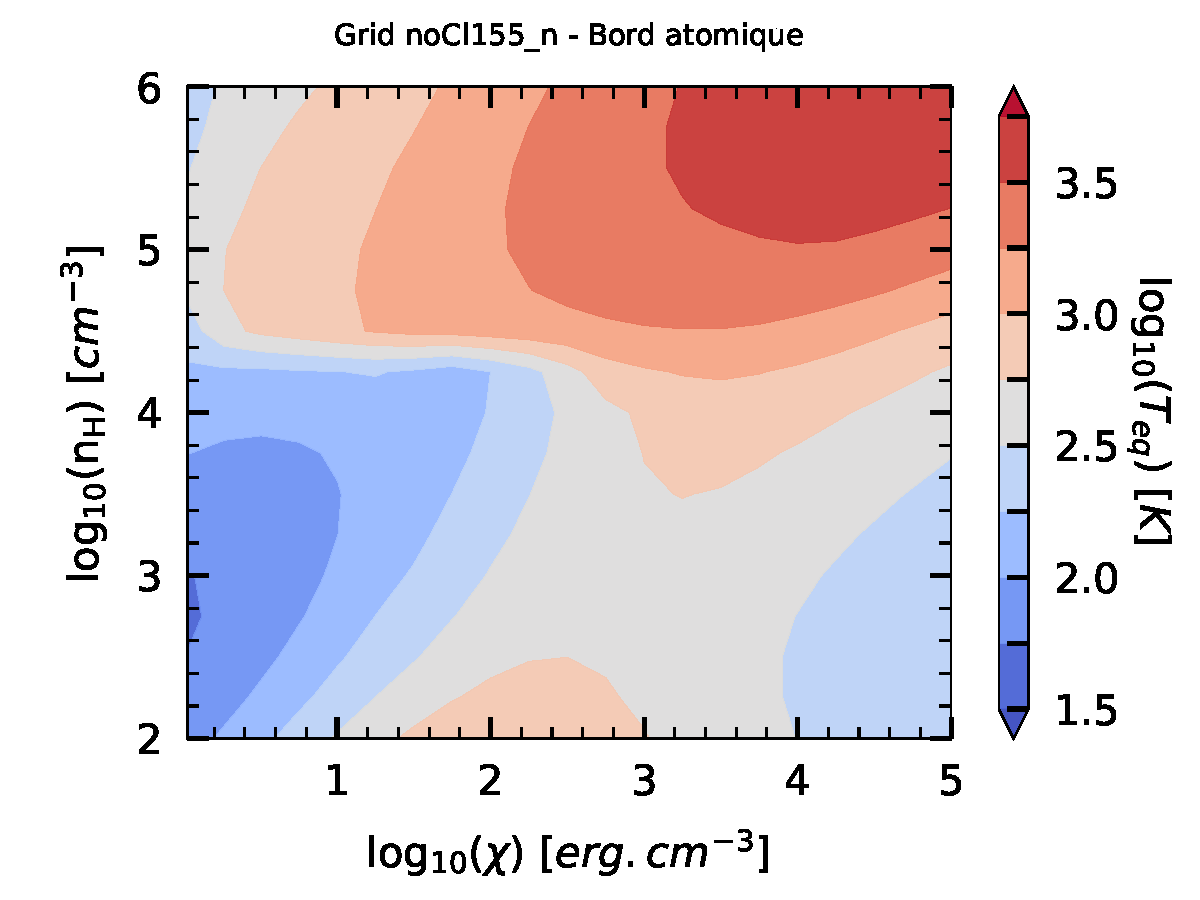
\includegraphics[trim = {0 0 0 1cm},clip,width=1\textwidth]{figure/Cl/gridnoCl155_n/mapTba.pdf}
        \caption{sans chlore}
        \label{fig:Cl:grid:Tba:noCl}
    \end{subfigure}
    \caption{Température en bord atomique de nuage calculé par le code PDR de Meudon}
    \label{fig:Cl:grid:Tba}
\end{figure}

Enfin, l'absence du $\mathrm{H}_2$ dans le modèle thermico-chimique a un impact important sur la température car il chauffe efficacement le gaz par pompage UV dans les régions denses et est également capable de refroidir par désexcitation collisionelle. On voit le voit sur la figure \ref{fig:Cl:particulier:4} où l'effet photoélectrique est devant le chauffage par $\mathrm{H}_2$. La molécule imprime la carte de température dans les régions diffuses et peu illuminées ainsi que dans les régions denses. 


% \begin{figure}[!h]
%     \centering
%     \begin{subfigure}[t]{0.49\textwidth} % "0.49" donne ici la largeur de l'image
%         \centering 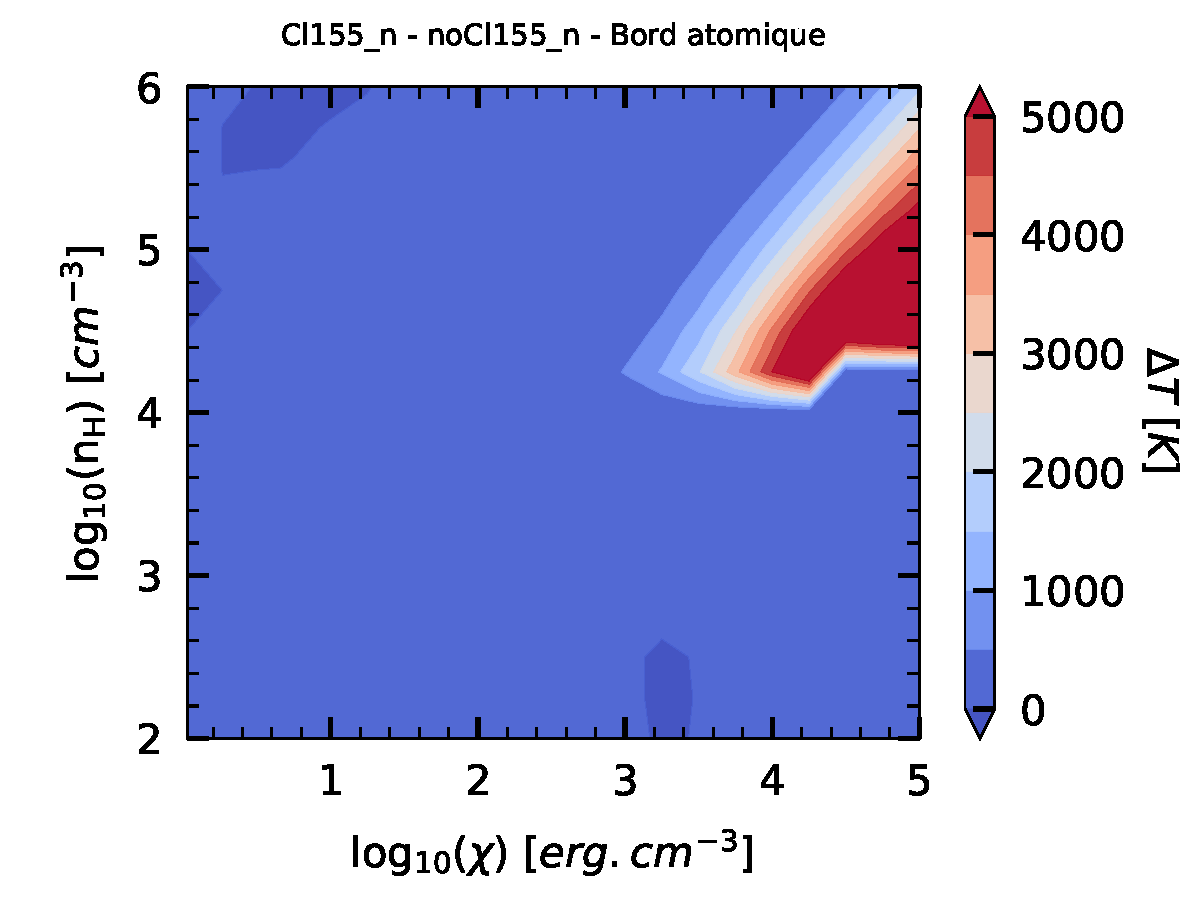
\includegraphics[trim = {0 0 0 1cm},clip,width=1\textwidth]{figure/Cl/gridCl155_n/mapTba_Cl155_n_noCl155_n.pdf}
%         \caption{différence de température en bord atomique}
%         \label{fig:Cl:grid:Tdiff}
%     \end{subfigure}
%     ~ 
%     \begin{subfigure}[t]{0.49\textwidth}
%         \centering 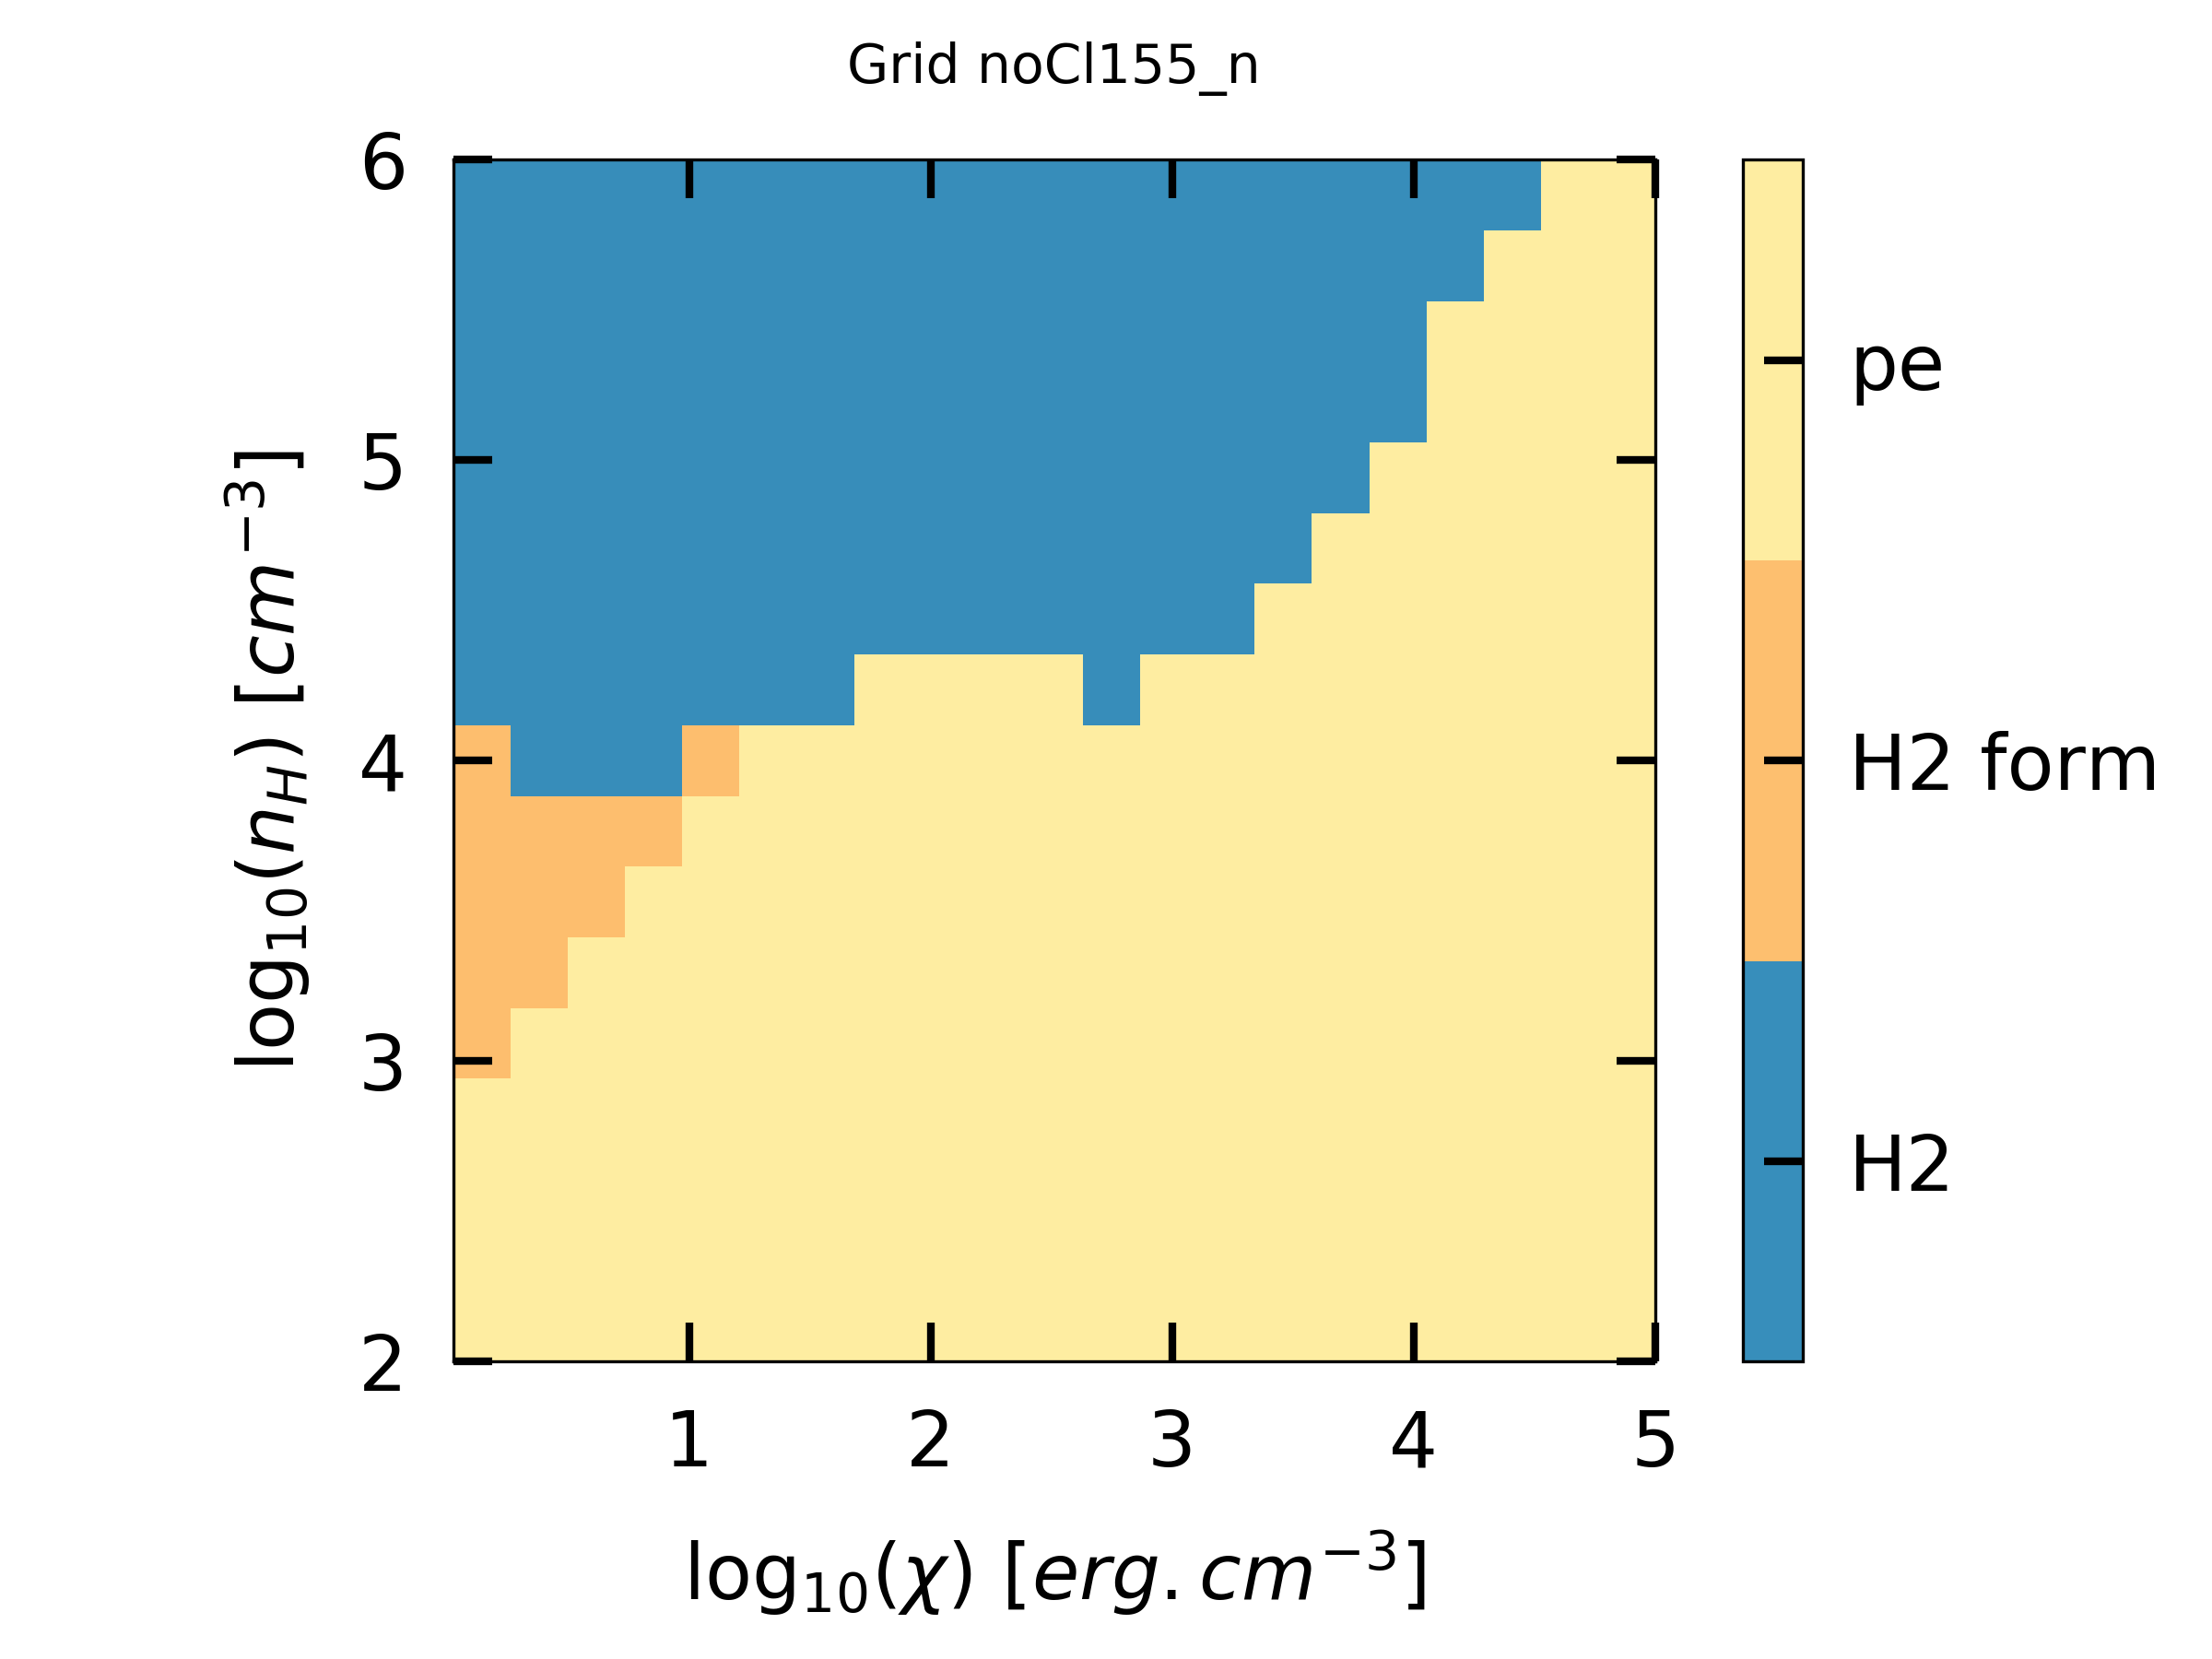
\includegraphics[trim = {0 0 0 1cm},clip,width=1\textwidth]{figure/Cl/gridnoCl155_n/mapGmax.png}
%         \caption{Processus de chauffage dominant en bord de nuage}
%         \label{fig:Cl:grid:Gmax}
%     \end{subfigure}
%     \caption{}
% \end{figure}


\begin{figure}[!h]
    \centering
    \begin{subfigure}[t]{0.49\textwidth} % "0.49" donne ici la largeur de l'image
        \centering 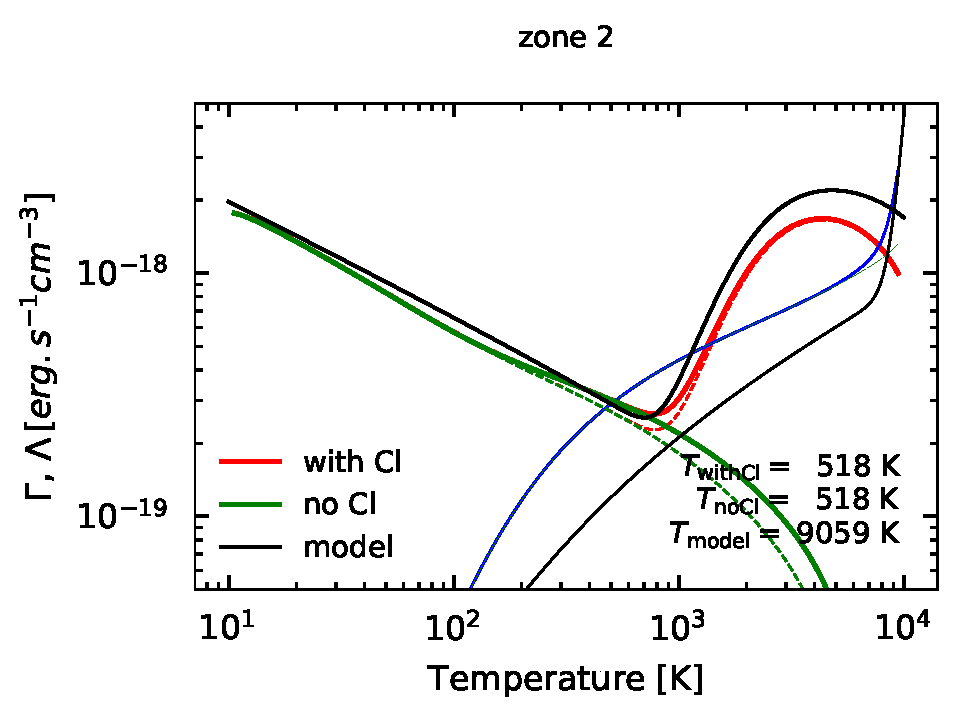
\includegraphics[trim = {0 0 0 1cm },clip,width=1\textwidth]{figure/Cl/particuliers/GCcomp_Cl_2.pdf}
        \caption{$n_\mathrm{H}=10^4 \, \mathrm{cm}^{-3}$, $\chi=10^{4.5}$ (zone 2)}
        \label{fig:Cl:particulier:2}
    \end{subfigure}
    ~ 
    \begin{subfigure}[t]{0.49\textwidth}
        \centering 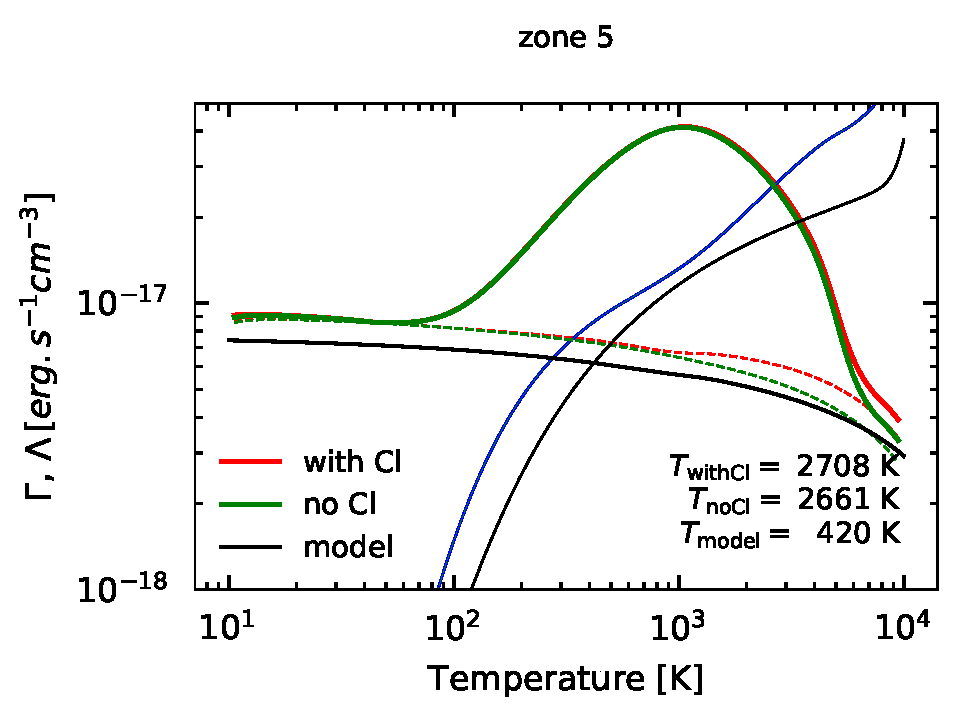
\includegraphics[trim = {0 0 0 1cm },clip,width=1\textwidth]{figure/Cl/particuliers/GCcomp_Cl_5.pdf}
        \caption{$n_\mathrm{H}=10^3 \, \mathrm{cm}^{-3}$, $\chi=10^3$ (zone 5)}
        \label{fig:Cl:particulier:4}
    \end{subfigure}
    \caption{Courbes de chauffage et refroidissement, au bord atomique de nuage, de modèles résolus par le code PDR de Meudon. Mêmes règles de couleurs que dans la figure \ref{fig:Cl:modelPE:GC}.}
\end{figure}



%%%%%%%%%%%%%%%%%%%%%%%%%%%%%%%%%%%%%%%%%%%%%%%%%%%%%%%%%%%%%%%%%%%%%%%%%%%%%%%%%%%%%%%%%

\subsection{A la recherche d'observables}

Nous avons pu prouver l'existence et expliquer le fonctionnement d'une instabilité provoqué par le chlore dans le bord atomique d'une PDR. Il est nécessaire de trouver des traceurs impactés ou des signatures dans les spectres d'émissions. \newline 

On choisit un modèle ($n_\mathrm{H}=10^5 \, \mathrm{cm}^{-3}$, $\chi=10^4.5$) dont le bord atomique devient nettement plus chaud lorsque l'on ajoute du chlore (figure \ref{fig:Cl:grid:Tba}). En traçant les spectres d'émission donnés par le code nous constatons que les raies $\mathrm{N}$, $\mathrm{N}^+$, $\mathrm{S}$, $\mathrm{Si}$ sont modifiées par la solution chaude (figure \ref{fig:Cl:gridModelEmiss:yes}). La présence du chlore augmente les raies du $\mathrm{N}$, $\mathrm{N}^+$ et $\mathrm{Si}$ d'un facteur 10 et du $\mathrm{S}$ d'un facteur 100. Le chlore opère un grand changement sur certaines raies mais il y a néanmoins un "seuil" d'observabilité des modèles PDR qui est de l'ordre de $10^{-6} \ \mathrm{erg}\,\mathrm{cm}^{-2}\,\mathrm{s}^{-1}$. Seules certaines raies du $\mathrm{N}$ sont supérieures à ce seuil. Les raies des autres traceurs, $\mathrm{CS}$, $\mathrm{H}_2\mathrm{O}$, $\mathrm{H}_2$, ne deviennent pas plus intense avec la solution chaude, certaines diminuent même (figure \ref{fig:Cl:gridModelEmiss:no}). \newline

\begin{figure}[!h]
    \centering
    \begin{subfigure}[t]{0.49\textwidth} % "0.49" donne ici la largeur de l'image
        \centering 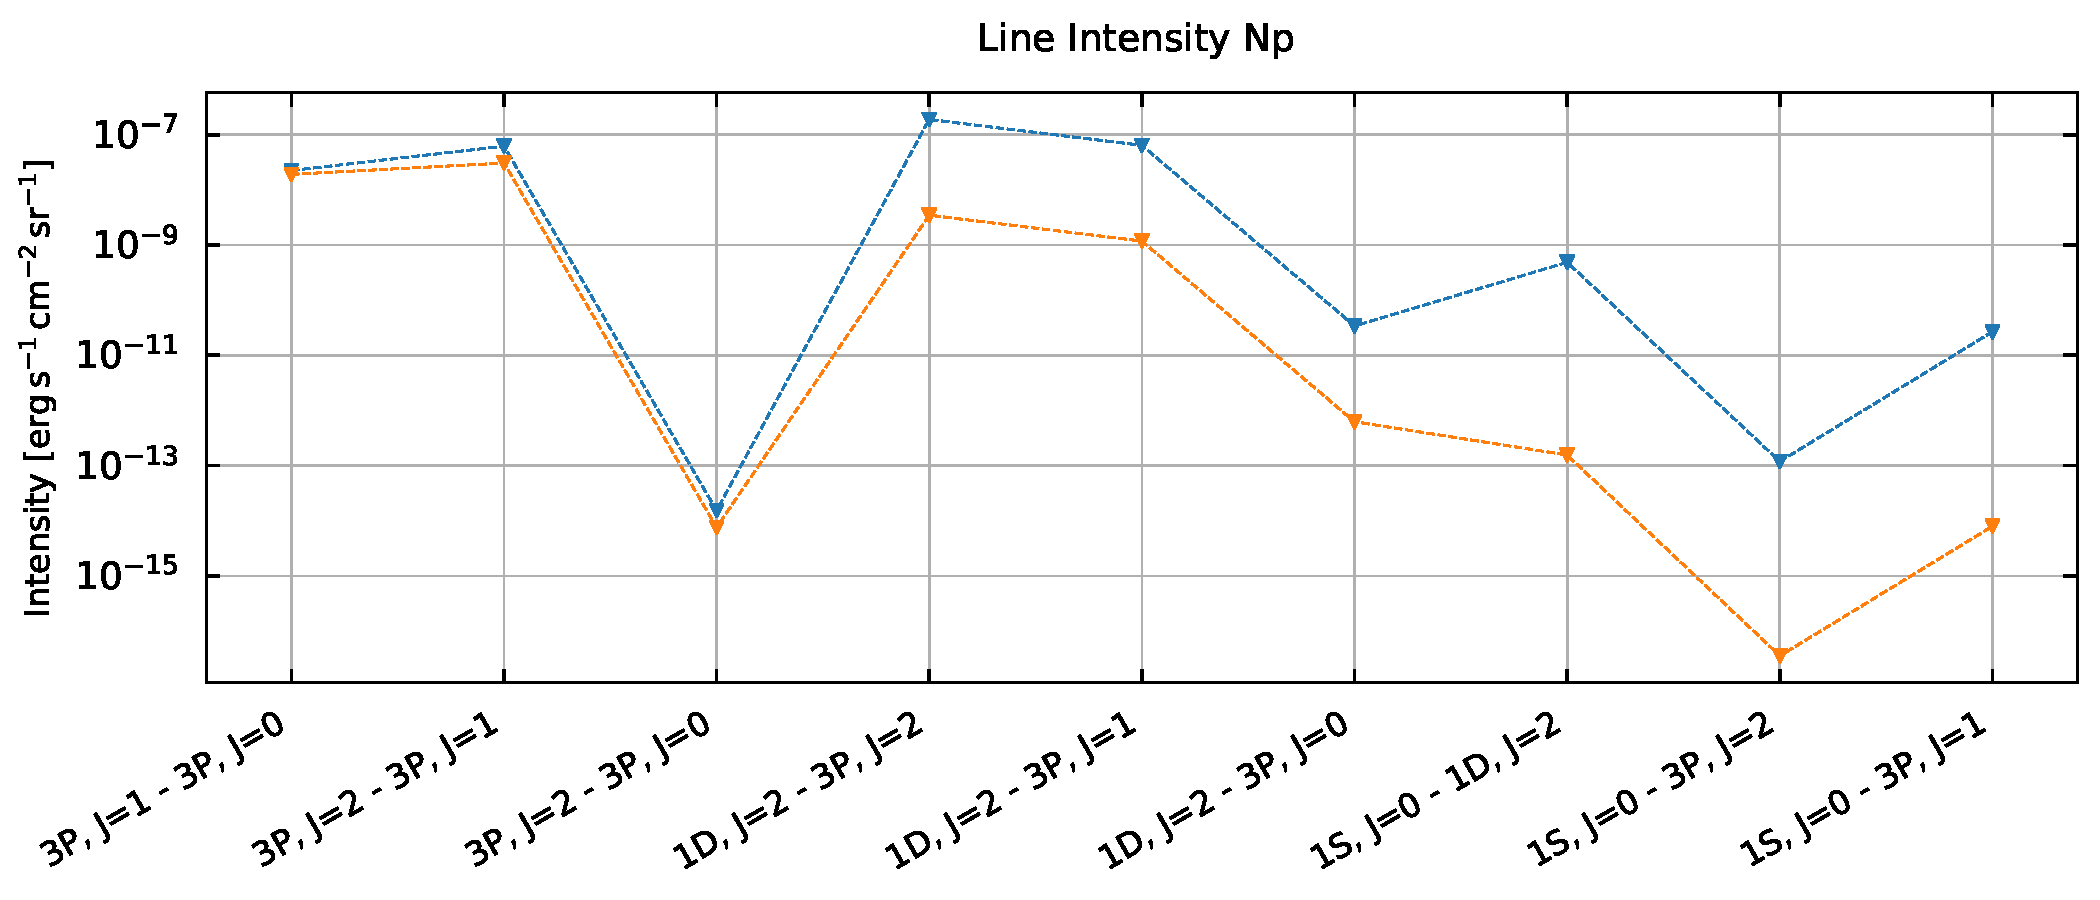
\includegraphics[trim = {0 0 0 1cm},clip,width=1\textwidth]{figure/Cl/gridModelEmiss/I_comp_Np.pdf}
        \caption{$\mathrm{N}^+$}
    \end{subfigure}
    ~ 
   \begin{subfigure}[t]{0.49\textwidth} % "0.49" donne ici la largeur de l'image
        \centering 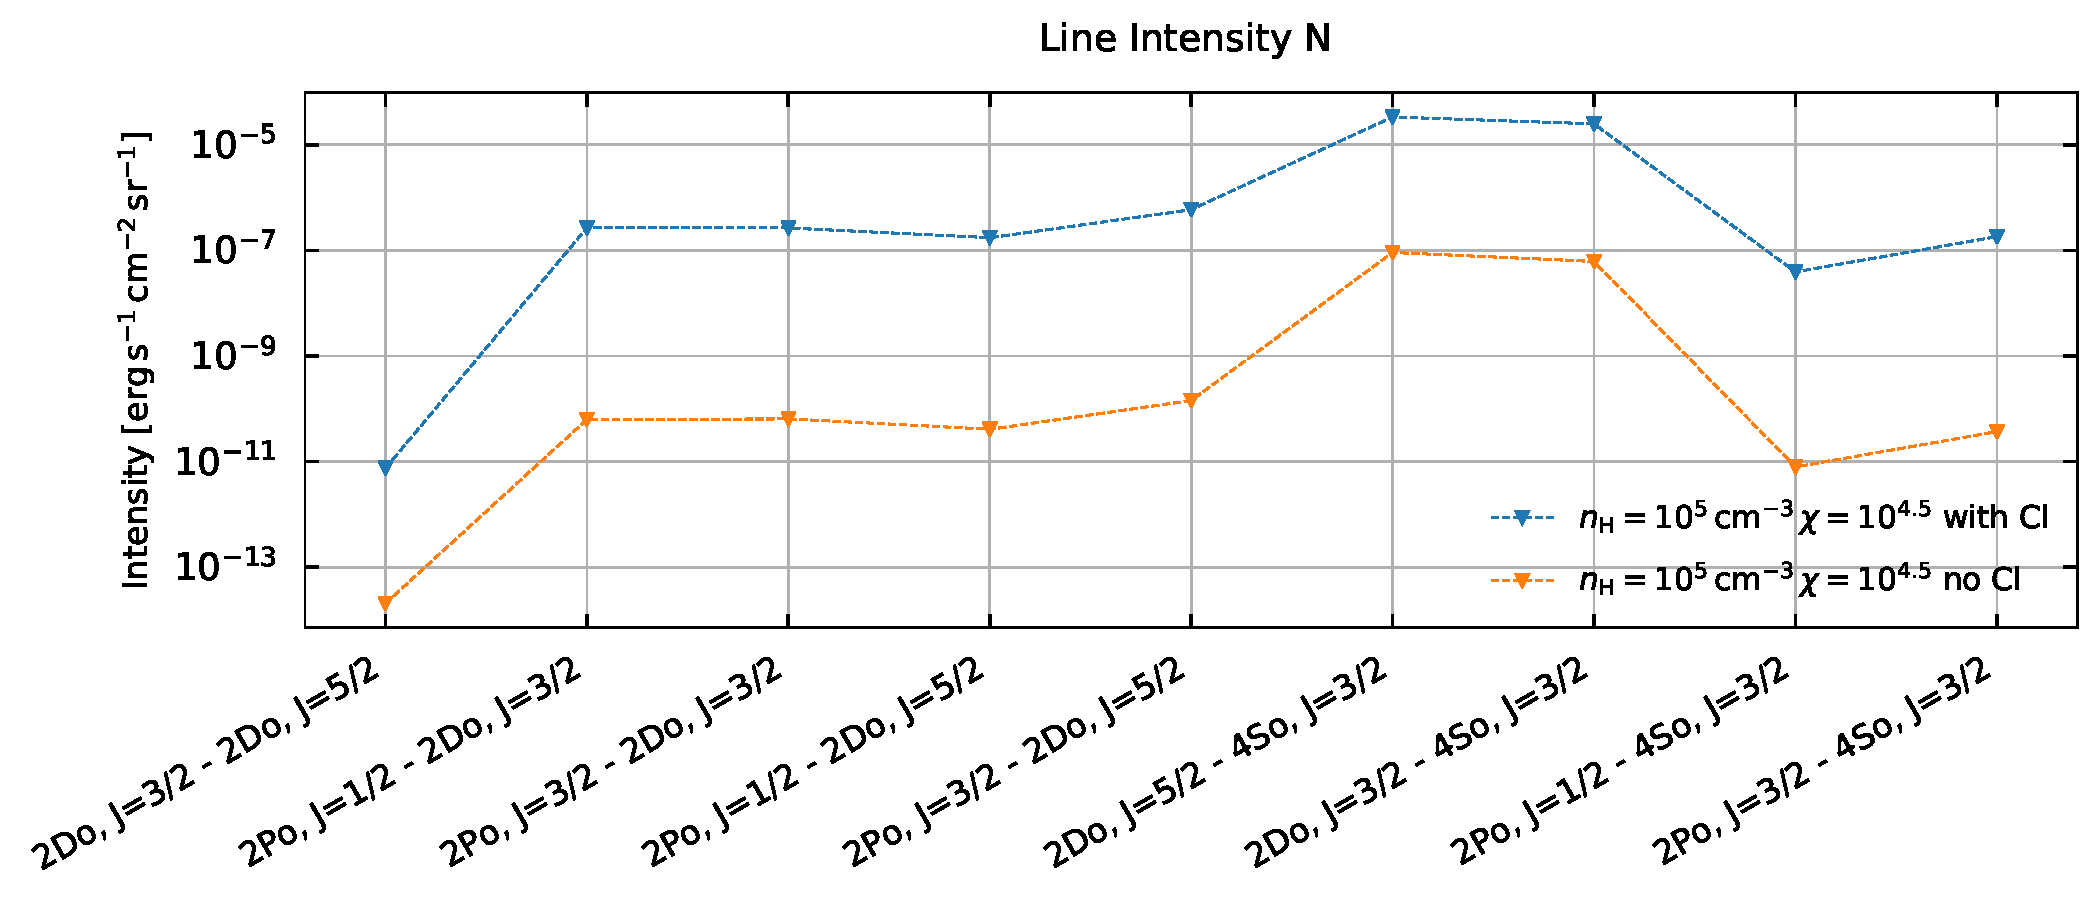
\includegraphics[trim = {0 0 0 1cm},clip,width=1\textwidth]{figure/Cl/gridModelEmiss/I_comp_N.pdf}
        \caption{$\mathrm{N}$}
    \end{subfigure}
    
    \begin{subfigure}[t]{0.49\textwidth} % "0.49" donne ici la largeur de l'image
        \centering 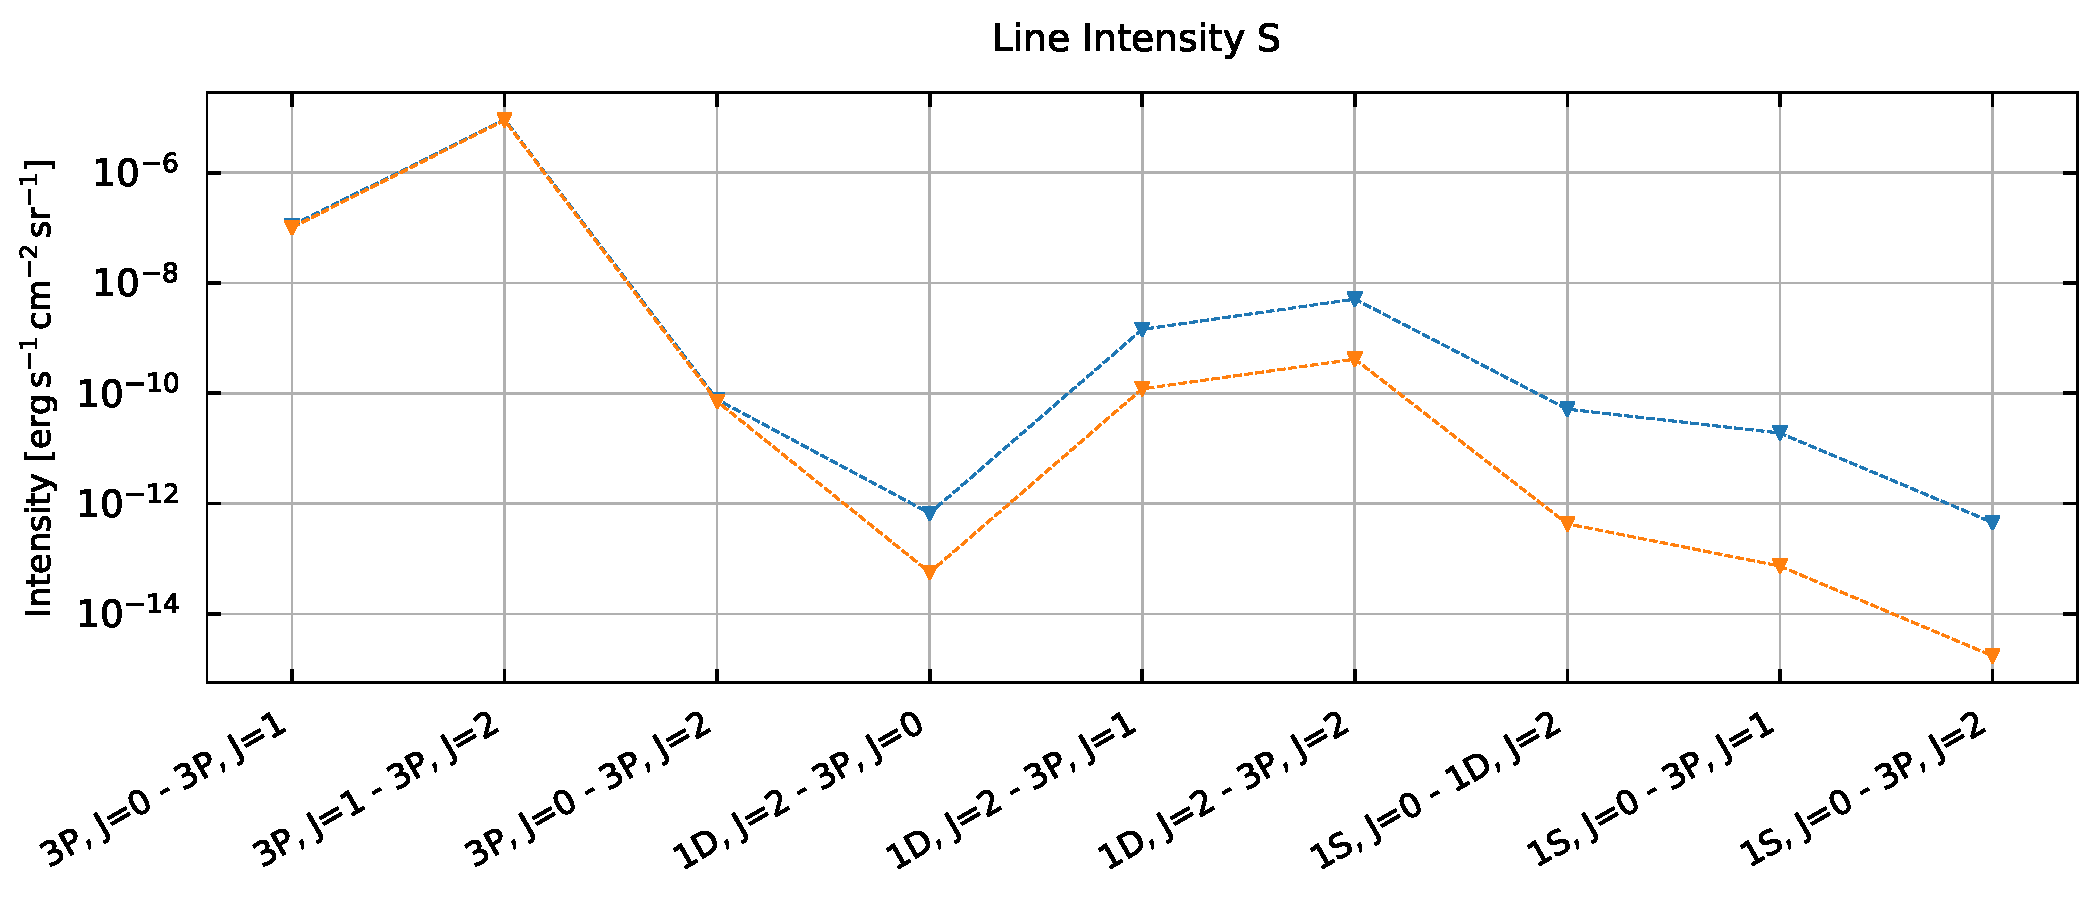
\includegraphics[trim = {0 0 0 1cm},clip,width=1\textwidth]{figure/Cl/gridModelEmiss/I_comp_S.pdf}
        \caption{$\mathrm{S}$}
    \end{subfigure}
    ~
    \begin{subfigure}[t]{0.49\textwidth} % "0.49" donne ici la largeur de l'image
        \centering 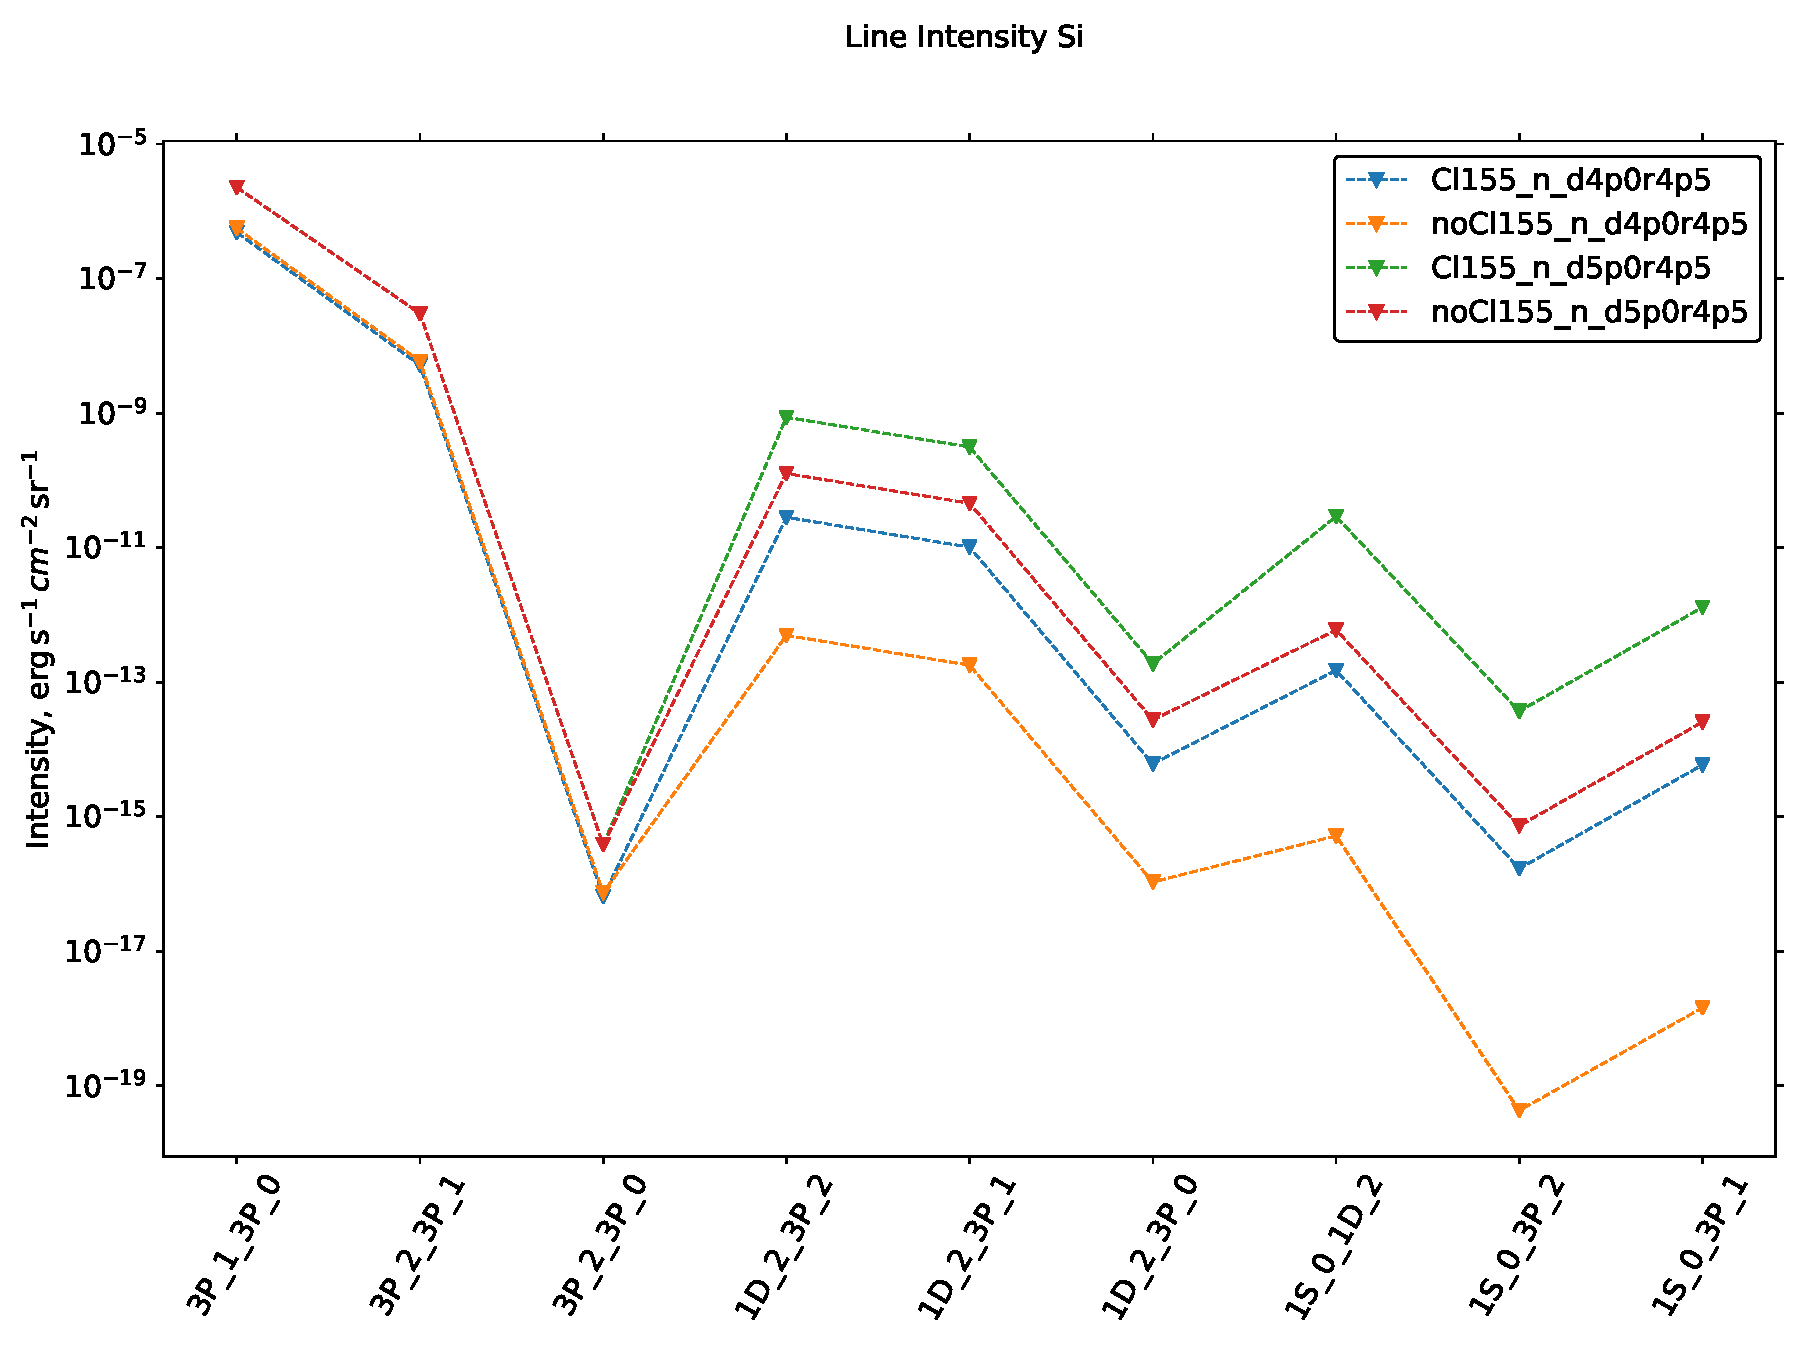
\includegraphics[trim = {0 0 0 1cm},clip,width=1\textwidth]{figure/Cl/gridModelEmiss/I_comp_Si.pdf}
        \caption{$\mathrm{Si}$}
    \end{subfigure}
    
    \caption{Diagramme d'excitation des traceurs modifiés par l'ajout du chlore.}
    \begin{minipage}{\textwidth}
    Les traits en bleue et orange sont les modèles $n_\mathrm{H}=10^5 \, \mathrm{cm}^{-3}$ et $\chi=10^{4.5}$ avec et sans le chlore (respectivement). Ces spectres sont affichés en plus grande taille dans l'annexe.
    \end{minipage}
    \label{fig:Cl:gridModelEmiss:yes}
\end{figure}

\begin{figure}[!h]
    \centering
    \begin{subfigure}[t]{0.49\textwidth} % "0.49" donne ici la largeur de l'image
        \centering 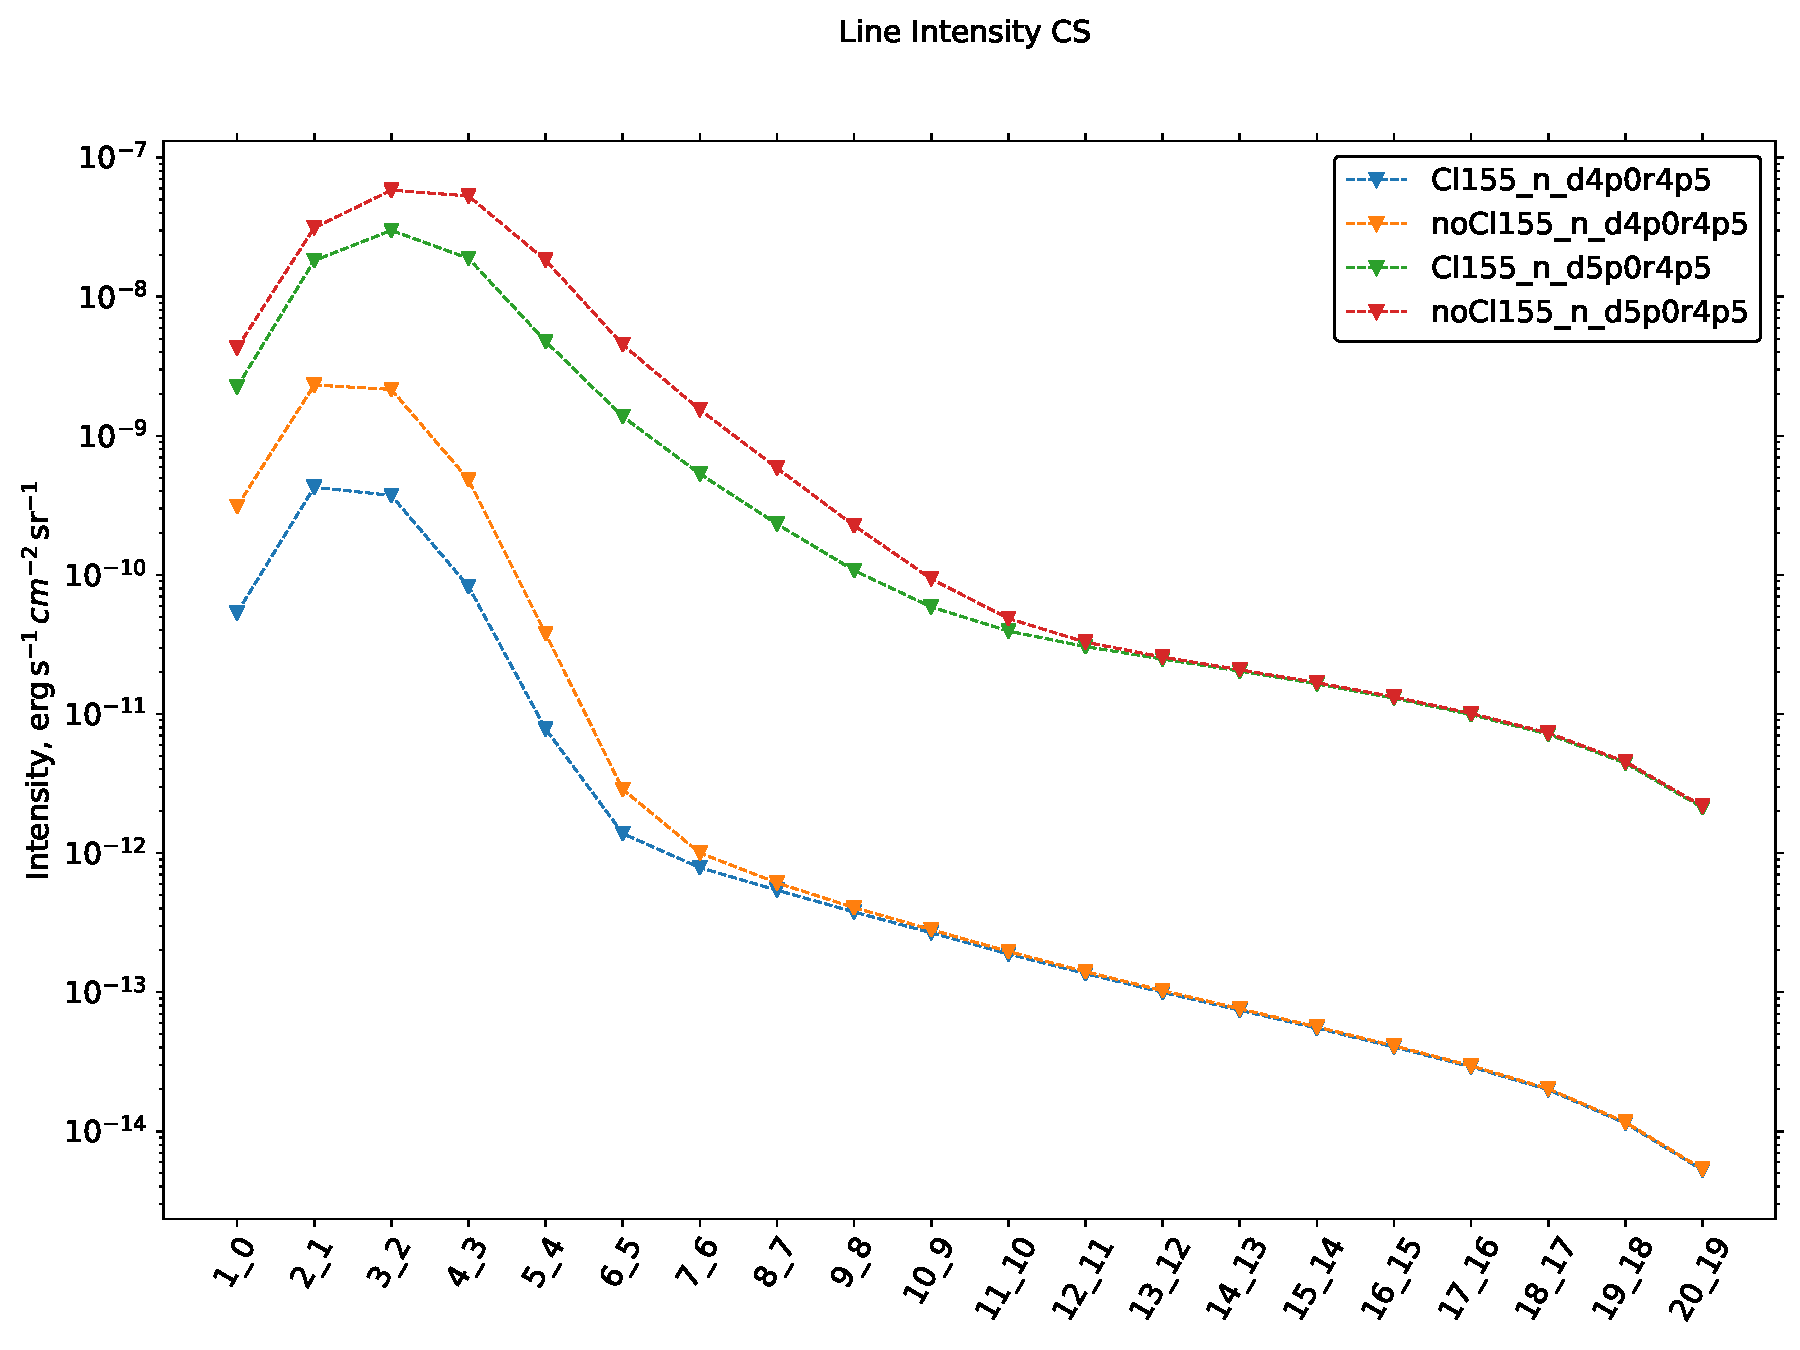
\includegraphics[trim = {0 0 0 1cm},clip,width=1\textwidth]{figure/Cl/gridModelEmiss/I_comp_CS.pdf}
        \caption{$\mathrm{CS}$}
    \end{subfigure}
    ~ 
   \begin{subfigure}[t]{0.49\textwidth} % "0.49" donne ici la largeur de l'image
        \centering 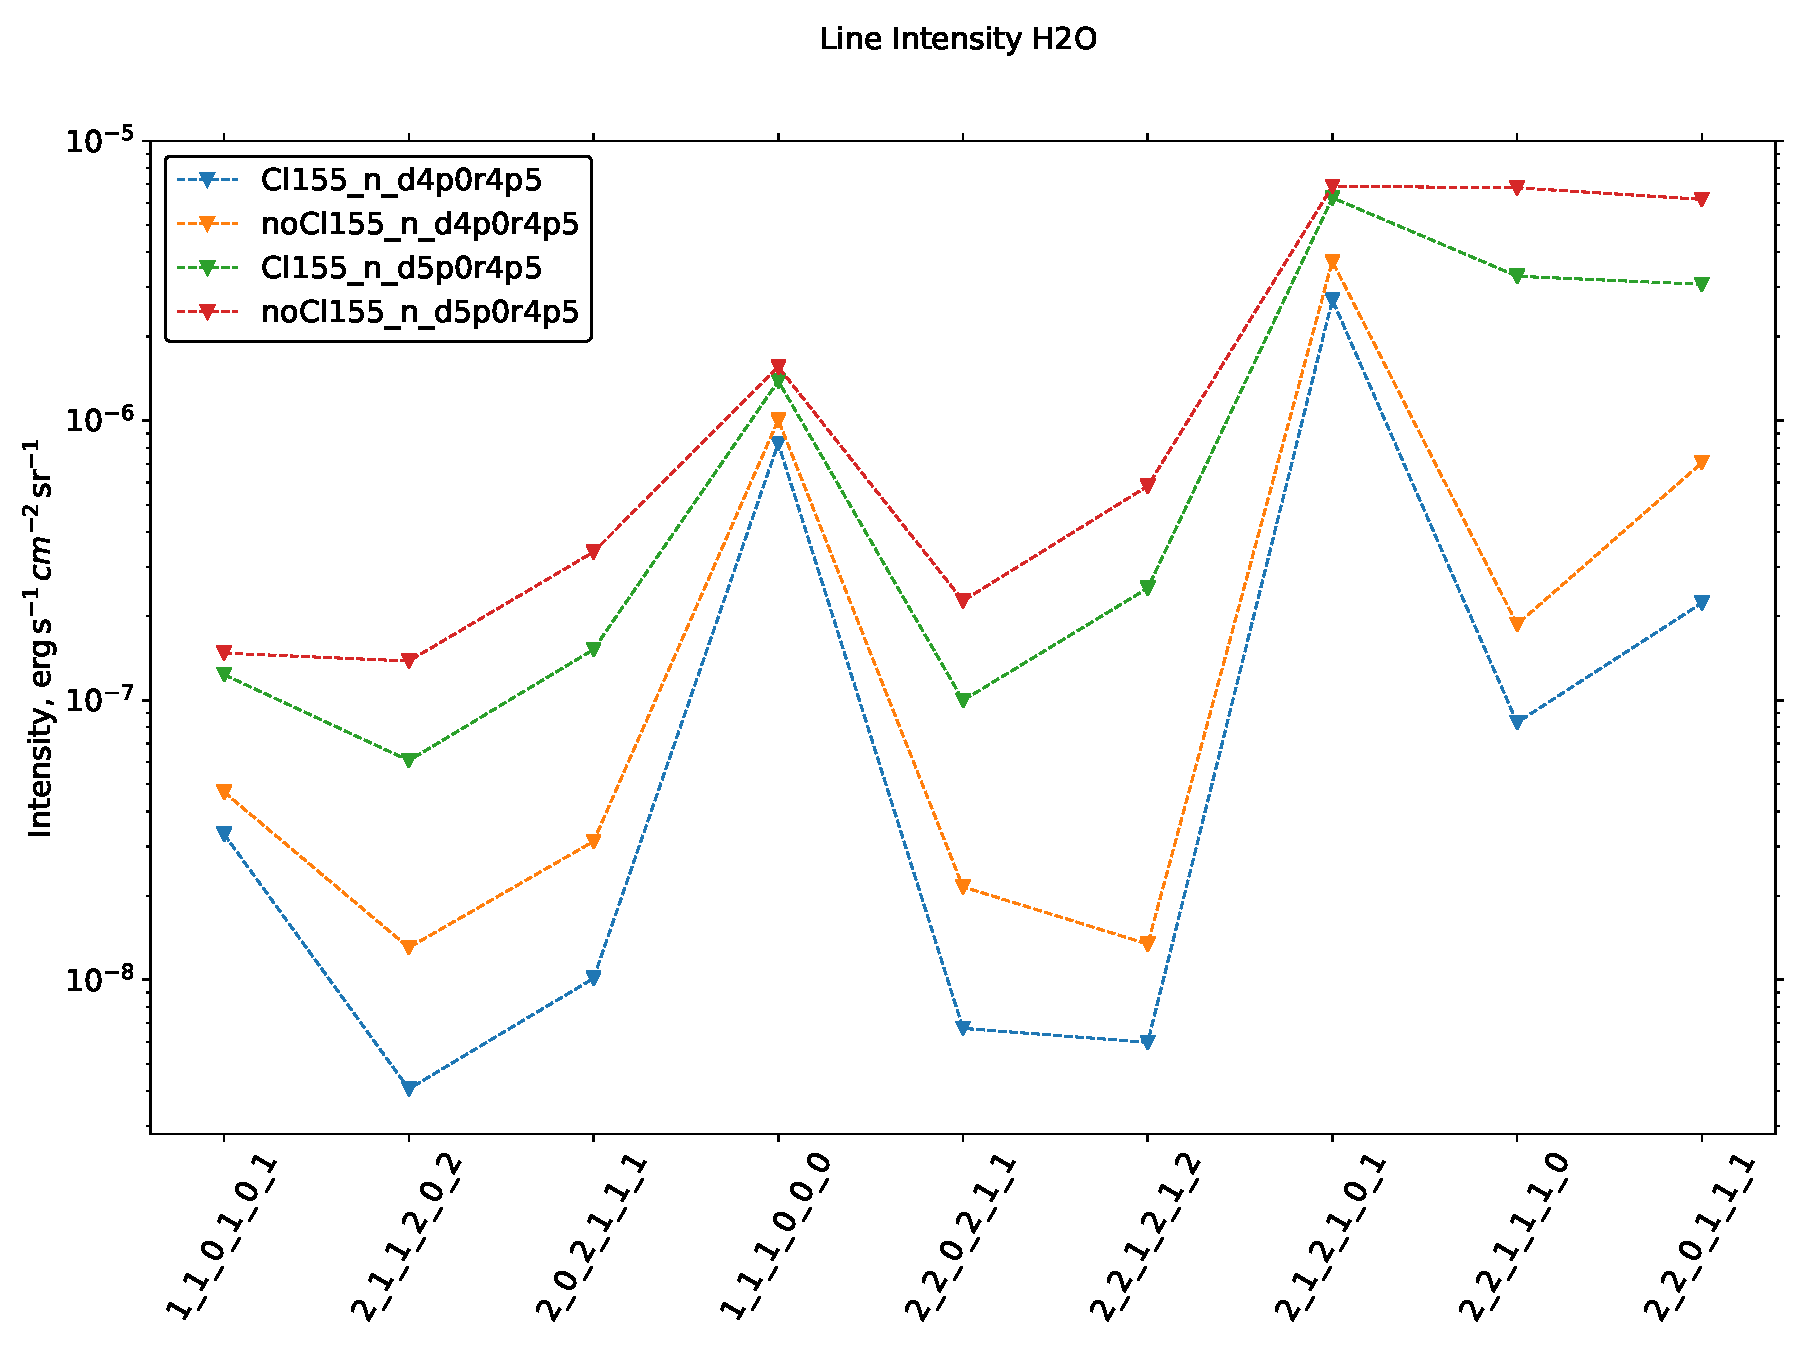
\includegraphics[trim = {0 0 0 1cm},clip,width=1\textwidth]{figure/Cl/gridModelEmiss/I_comp_H2O.pdf}
        \caption{$\mathrm{H}_2\mathrm{O}$}
    \end{subfigure}
    
    \begin{subfigure}[t]{0.49\textwidth} % "0.49" donne ici la largeur de l'image
        \centering 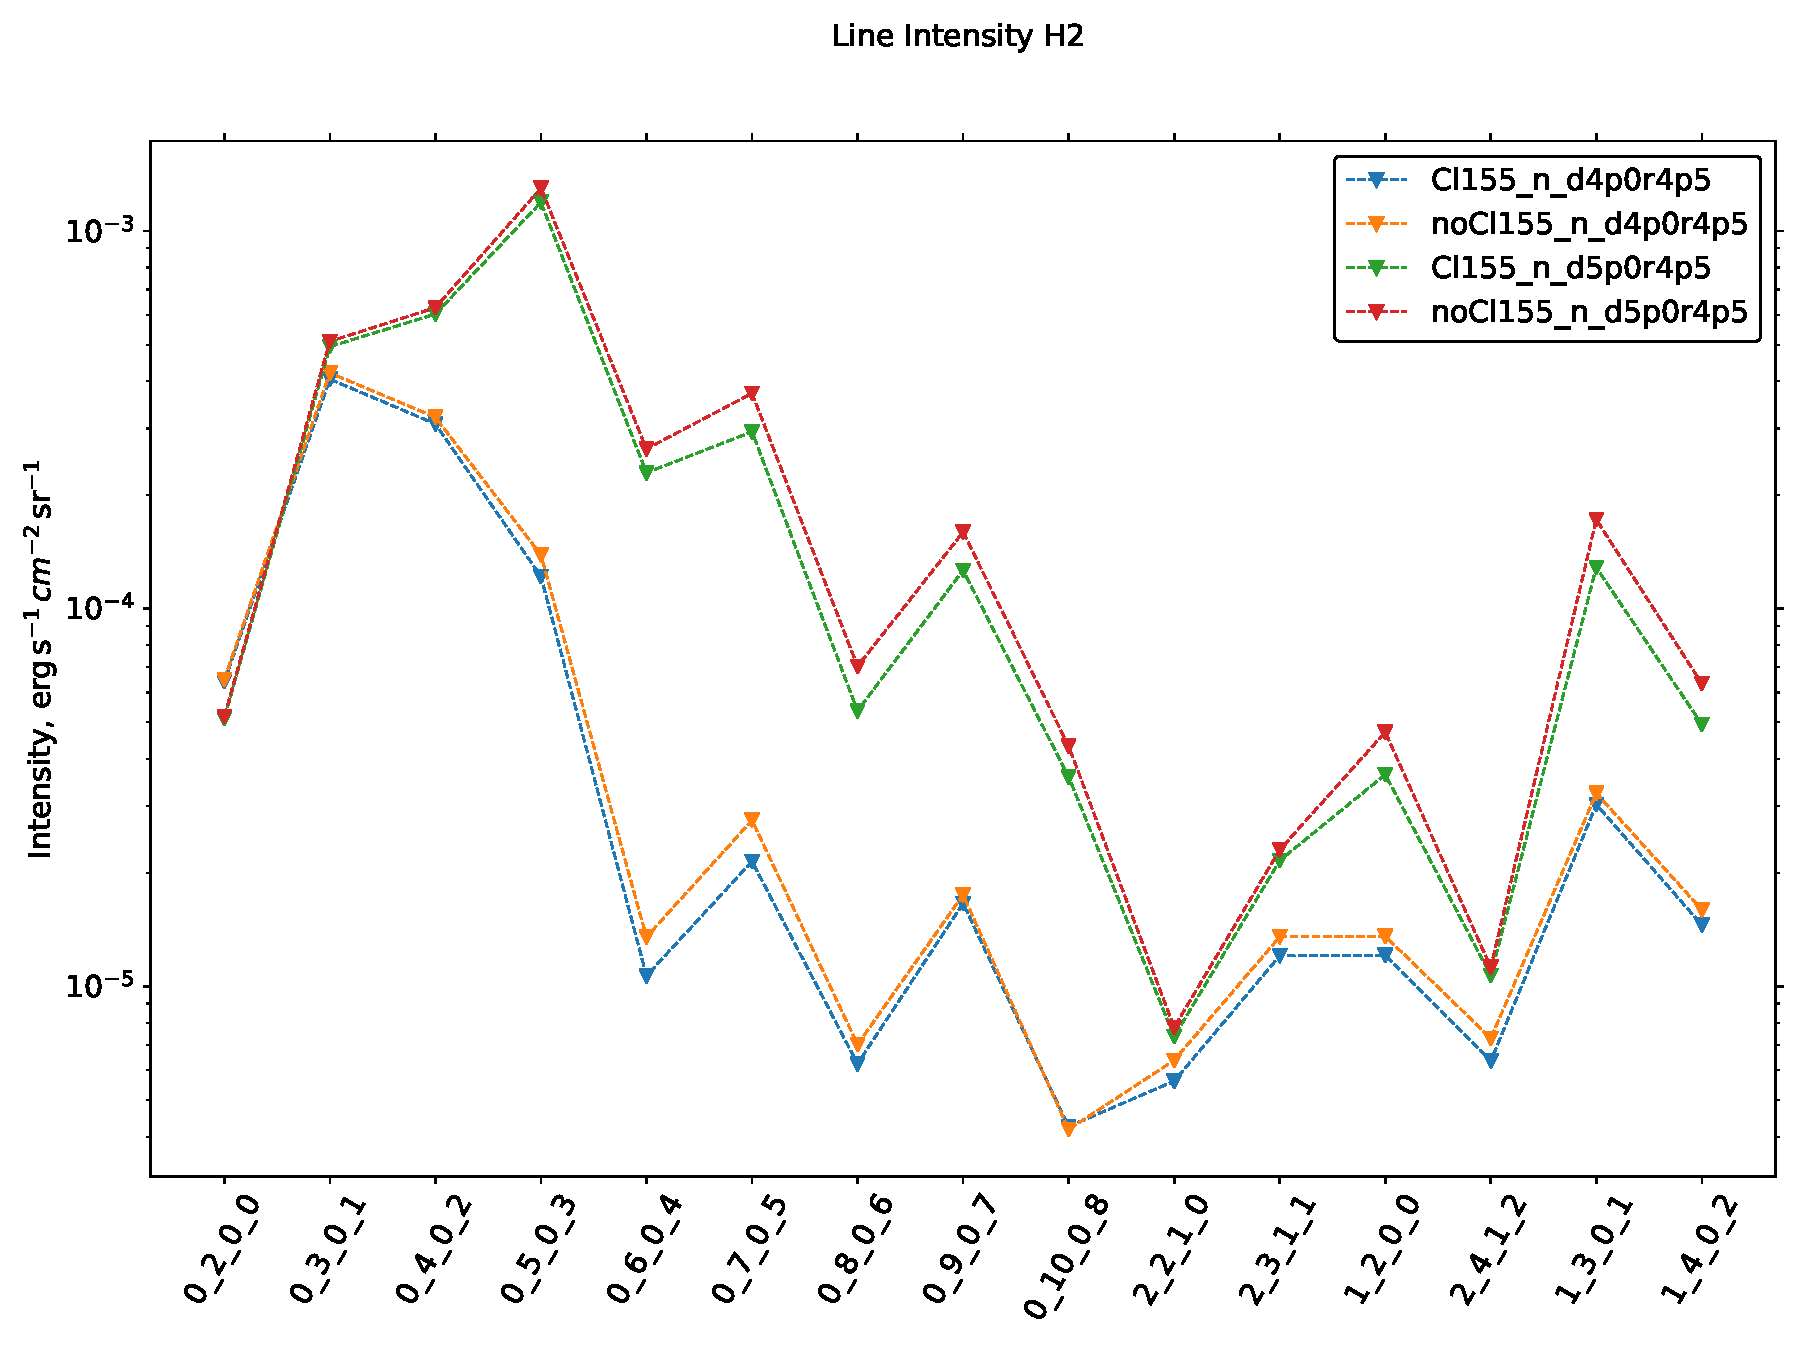
\includegraphics[trim = {0 0 0 1cm},clip,width=1\textwidth]{figure/Cl/gridModelEmiss/I_comp_H2.pdf}
        \caption{$\mathrm{H}_2$}
    \end{subfigure}
    ~ 
    \begin{subfigure}[t]{0.49\textwidth} % "0.49" donne ici la largeur de l'image
        \centering 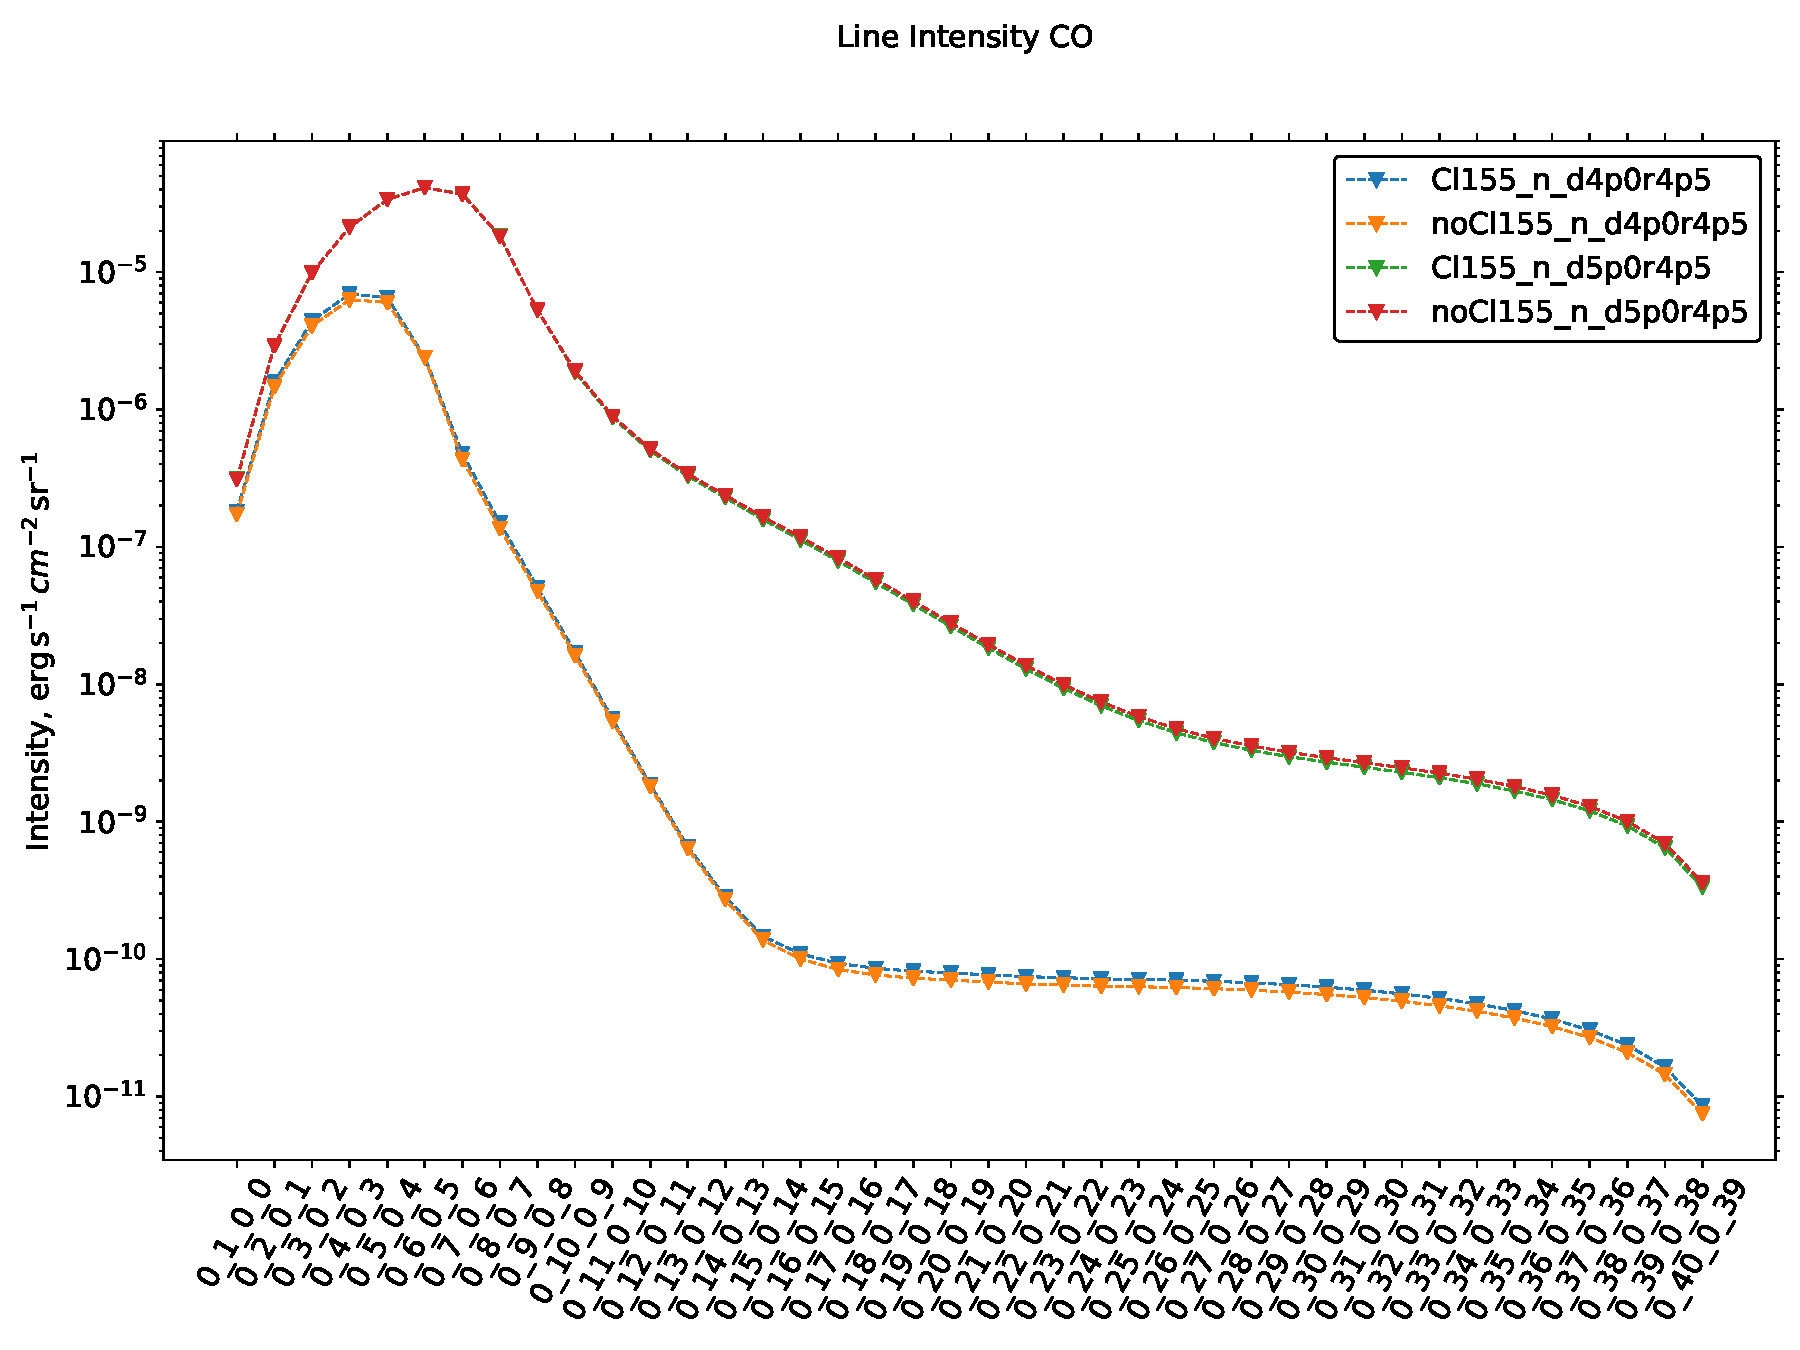
\includegraphics[trim = {0 0 0 1cm},clip,width=1\textwidth]{figure/Cl/gridModelEmiss/I_comp_CO.pdf}
        \caption{$\mathrm{CO}$}
    \end{subfigure}
    
    \caption{(ANNEXE) Diagramme d'excitation des traceurs peu modifiés par l'ajout du chlore dans le code PDR (même convention que la figure \ref{fig:Cl:gridModelEmiss:yes}). Pour la molécule $\mathrm{CO}$, les transitions rotationnelles ont été écrites (toutes s'effectuent à $\mathrm{v}=0$.}
    \label{fig:Cl:gridModelEmiss:no}
\end{figure}


% \subsubsection{Profils de densités des traceurs}

\begin{figure}[!htbp]
    \centering
    \begin{subfigure}[t]{0.49\textwidth} % "0.49" donne ici la largeur de l'image
        \centering 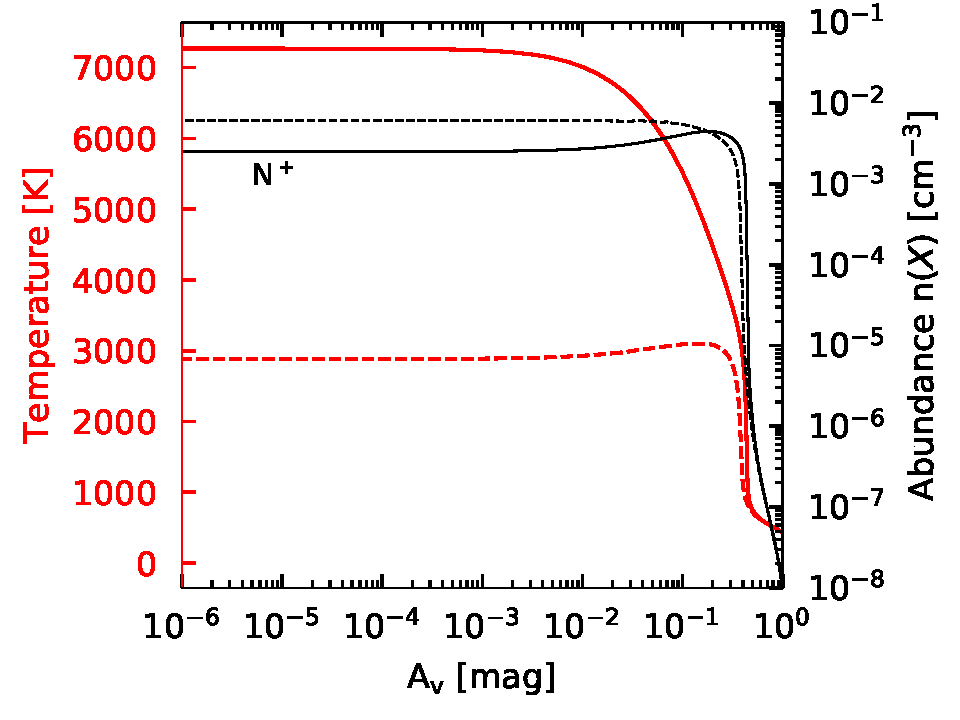
\includegraphics[trim = {0 0 0 0},clip,width=1\textwidth]{figure/Cl/gridModelEmiss/nT_comp_Np.pdf}
        \caption{$\mathrm{N}^+$}
    \end{subfigure}
    ~ 
   \begin{subfigure}[t]{0.49\textwidth} % "0.49" donne ici la largeur de l'image
        \centering 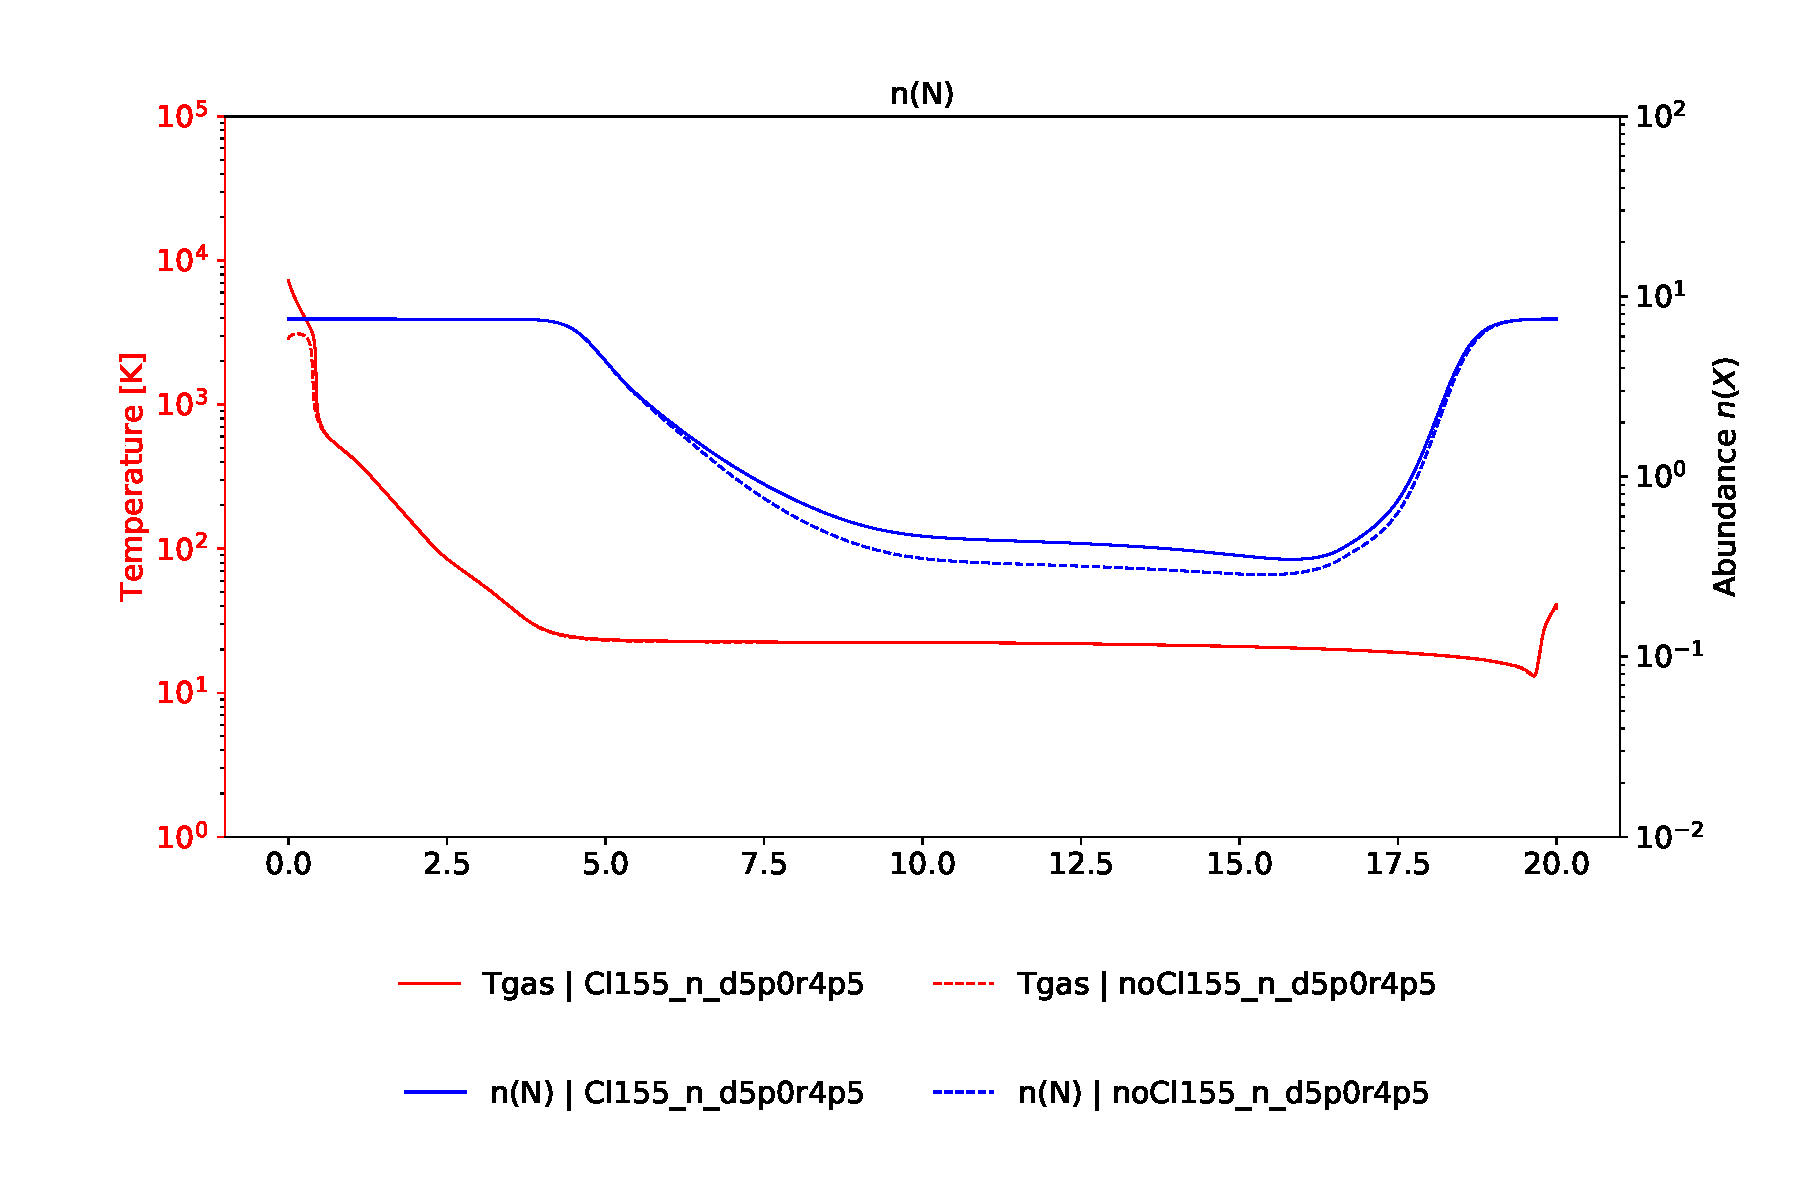
\includegraphics[trim = {0 0 0 0},clip,width=1\textwidth]{figure/Cl/gridModelEmiss/nT_comp_N.pdf}
        \caption{$\mathrm{N}$}
    \end{subfigure}
    
    \begin{subfigure}[t]{0.49\textwidth} % "0.49" donne ici la largeur de l'image
        \centering 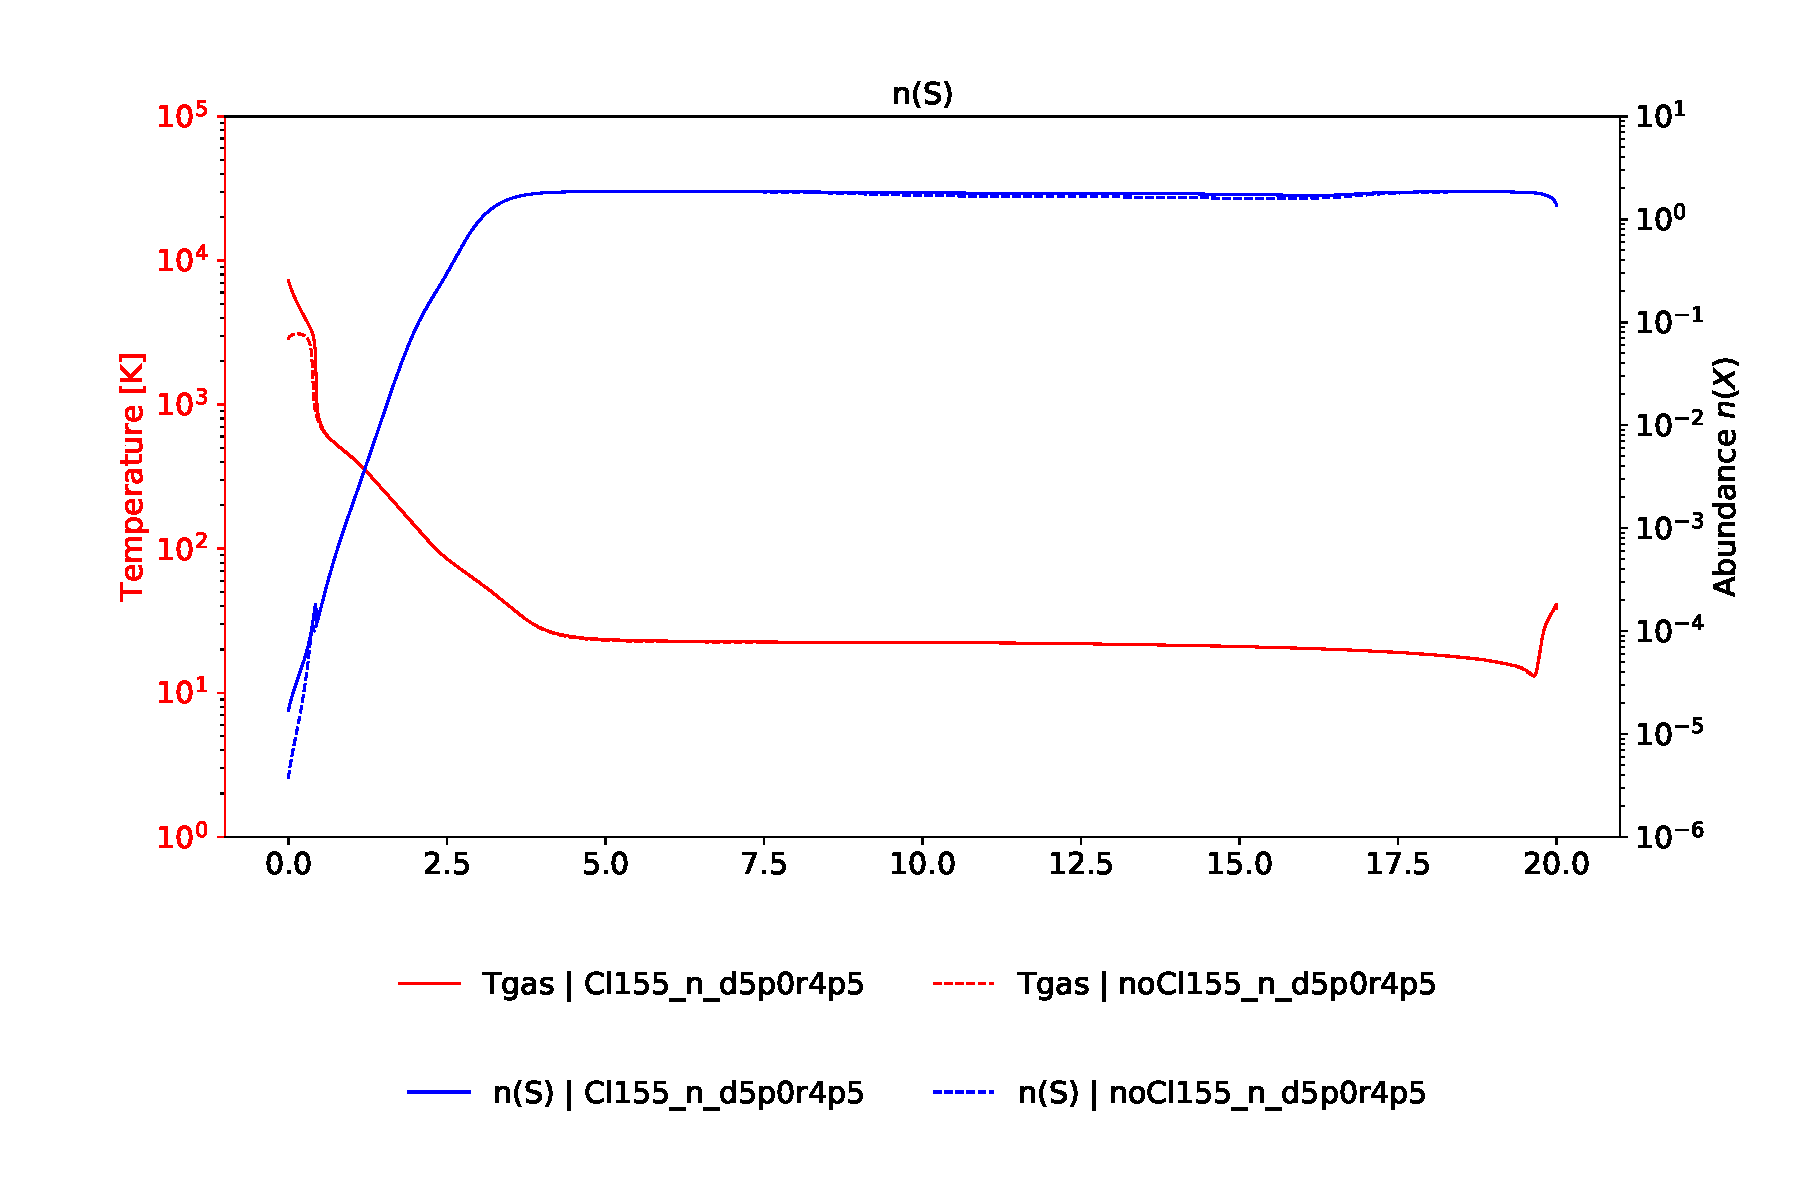
\includegraphics[trim = {0 0 0 0},clip,width=1\textwidth]{figure/Cl/gridModelEmiss/nT_comp_S.pdf}
        \caption{$\mathrm{S}$}
    \end{subfigure}
    ~
    \begin{subfigure}[t]{0.49\textwidth} % "0.49" donne ici la largeur de l'image
        \centering 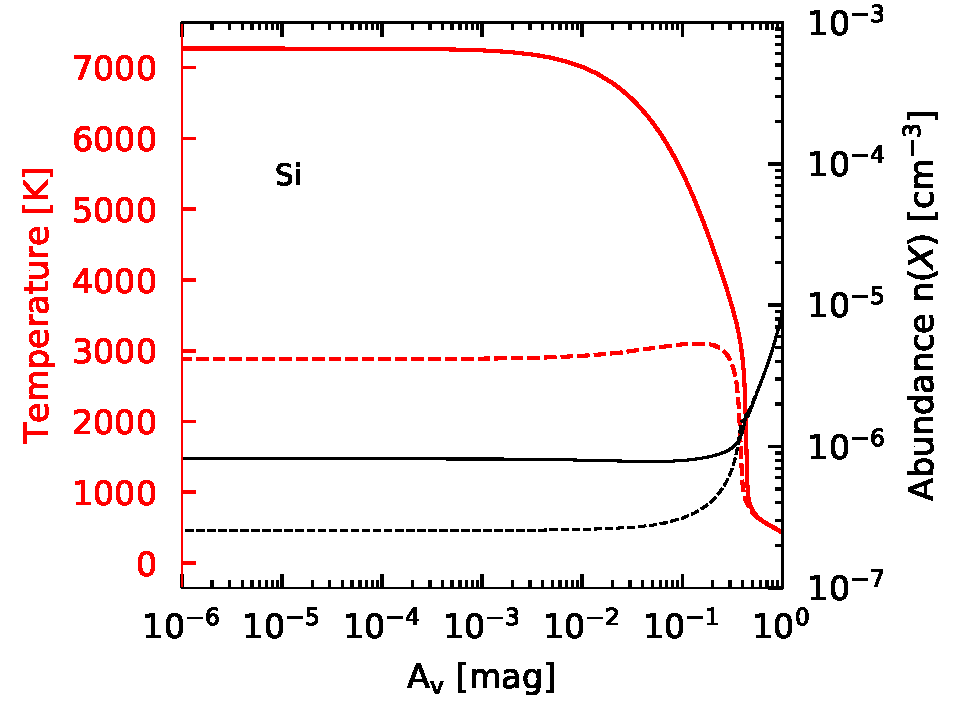
\includegraphics[trim = {0 0 0 0},clip,width=1\textwidth]{figure/Cl/gridModelEmiss/nT_comp_Si.pdf}
        \caption{$\mathrm{Si}$}
    \end{subfigure}
    
    \caption{(ANNEXE) Profils de densité des traceurs modifiés par l'ajout du chlore dans le code PDR (\uncinq)}
    \label{fig:Cl:gridModelEmiss:nT:yes}
\end{figure}

\begin{figure}[!htbp]
    \centering
    \begin{subfigure}[t]{0.49\textwidth} % "0.49" donne ici la largeur de l'image
        \centering 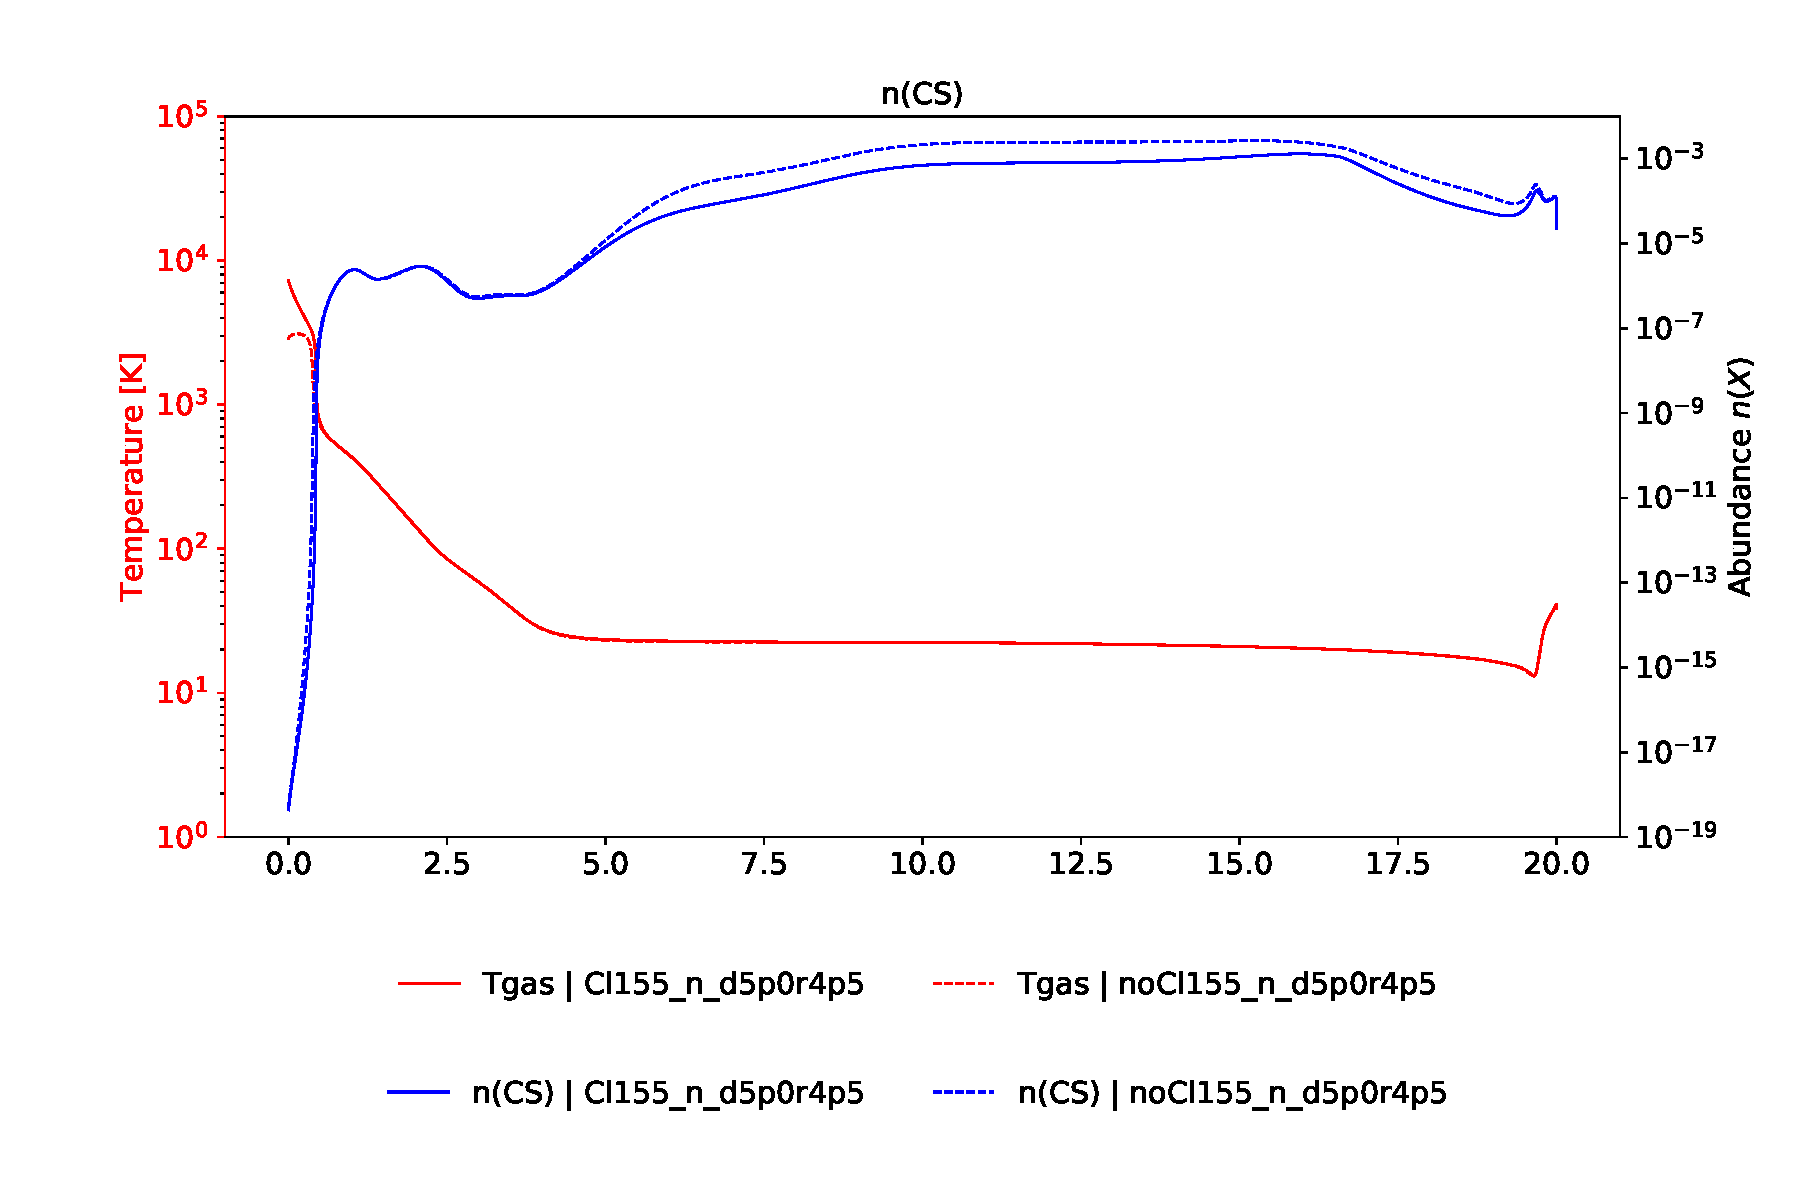
\includegraphics[trim = {0 0 0 0},clip,width=1\textwidth]{figure/Cl/gridModelEmiss/nT_comp_CS.pdf}
        \caption{$\mathrm{CS}$}
    \end{subfigure}
    ~ 
   \begin{subfigure}[t]{0.49\textwidth} % "0.49" donne ici la largeur de l'image
        \centering 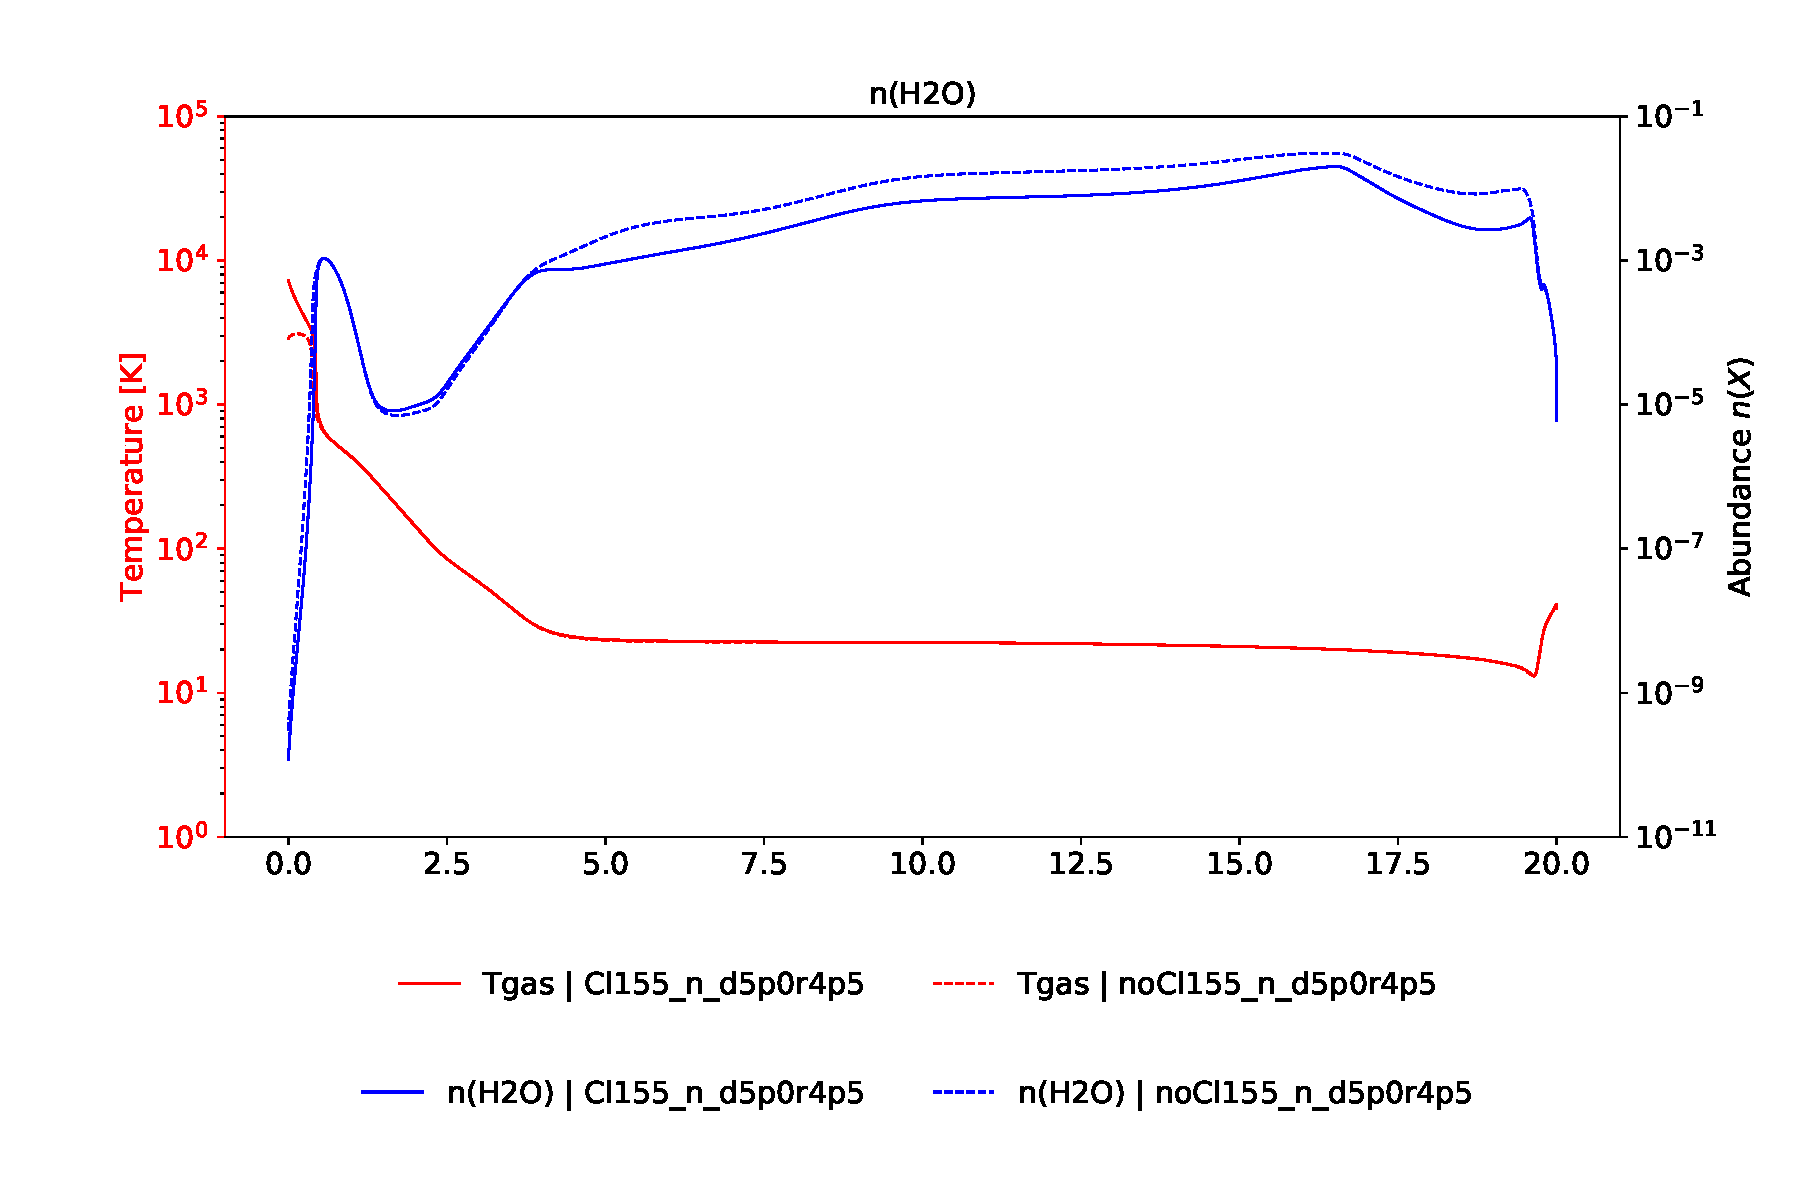
\includegraphics[trim = {0 0 0 0},clip,width=1\textwidth]{figure/Cl/gridModelEmiss/nT_comp_H2O.pdf}
        \caption{$\mathrm{H}_2\mathrm{O}$}
    \end{subfigure}
    
    \begin{subfigure}[t]{0.49\textwidth} % "0.49" donne ici la largeur de l'image
        \centering 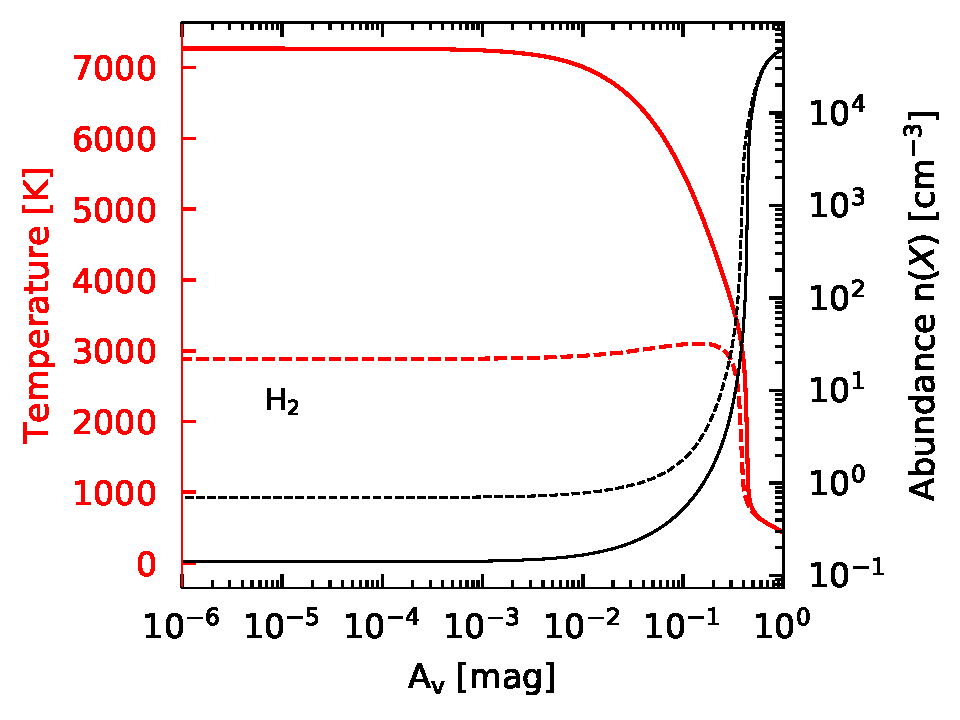
\includegraphics[trim = {0 0 0 0},clip,width=1\textwidth]{figure/Cl/gridModelEmiss/nT_comp_H2.pdf}
        \caption{$\mathrm{H}_2$}
    \end{subfigure}
    ~ 
    \begin{subfigure}[t]{0.49\textwidth} % "0.49" donne ici la largeur de l'image
        \centering 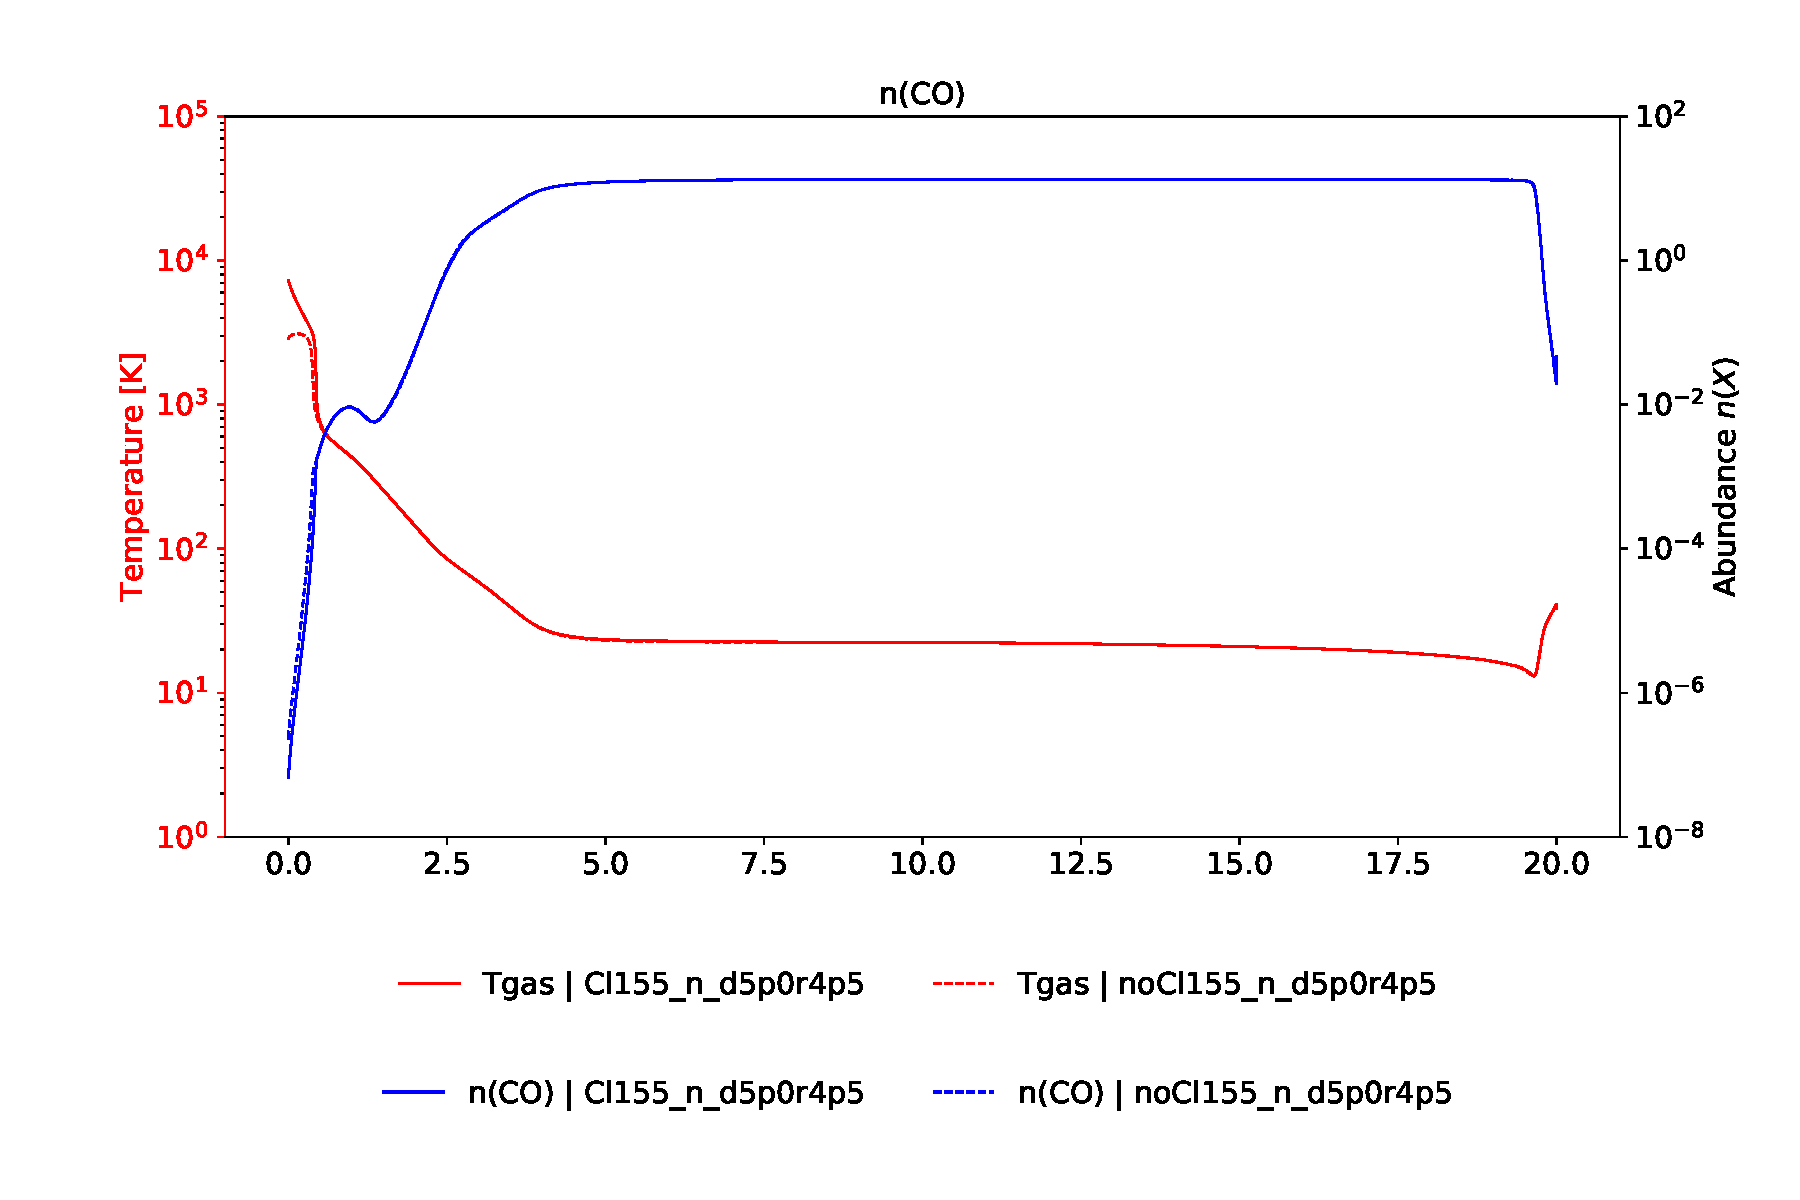
\includegraphics[trim = {0 0 0 0},clip,width=1\textwidth]{figure/Cl/gridModelEmiss/nT_comp_CO.pdf}
        \caption{$\mathrm{CO}$}
    \end{subfigure}
    
    \caption{(ANNEXE) Profil des densités des traceurs peu modifiés par l'ajout du chlore dans le code PDR (\uncinq)}
    \label{fig:Cl:gridModelEmiss:nT:no}
\end{figure}

\subsubsection{Choix de la raie [N] $5200 \mathrm{A}$}

Il a été dit précédemment que, d'après le code PDR, il serait possible d'observer seulement des raies du $\mathrm{N}$. On a choisit la raie la plus intense qui est la transition El=2Do,J=5/2 $\rightarrow$ El=4So,J=3/2 correspondant à la longueur d'onde $5200 \mathrm{A}$ appartenant au domaine du visible. <à finir>

On voit sur la figure \ref{fig:Cl:gridModelEmiss:N} que lorsque l'on a du chlore, l'intensité de la raie atteint est de l'ordre de $10^{-3} \mathrm{erg}\,\mathrm{cm}^{-2}\,\mathrm{s}^{-1}$ et que l'on a une signature de la solution chaude proposée par le chlore. Néanmoins la taille de la zone concernée est petite et il est difficile de bien situer les observations dans l'espace des paramètres. Un autre problème, qui n'est pas des moindres, est que les modèles de PDR commencent après la partir ionisé de l'hydrogène et que le potentiel de ionisation de l'azote est de $14.6 \ \mathrm{eV}$ ce qui signifie que la transition $\mathrm{N}^+/\mathrm{N}$ se fait devant le nuage. Dans le code, l'azote est excité par collision avec les espèces majoritaires du nuage qui sont $\mathrm{H}$,$\mathrm{H}^+$ $\mathrm{H}_2$, $\mathrm{He}$ et $e^-$ (PXDR\_COLSPE). La fraction électronique en bord atomique de nuage, dans le cas d'un emballement lié au chlore, est d'un facteur $10^{-4}$-$10^{-3}$ alors qu'il est d'un facteur 1 dans la partie ionisé du nuage. Cette augmentation de l'intensité de la raie sera masqué par le front $\mathrm{N}^+/\mathrm{N}$. \newline

Il faudrait donc trouver des traceurs qui ont des potentiels de ionisations inférieures à celui de l'hydrogène et qui s'activerait uniquement en bord atomique. Enfin on a tracé les diagrammes d'excitations avec des modèles à densités constantes qui corrobore rarement avec les données. Il faudrait lancer des grilles isobares et voir ce qu'il en est.


\begin{figure}[!htbp]
    \centering
    \begin{subfigure}[t]{0.49\textwidth} % "0.49" donne ici la largeur de l'image
        \centering 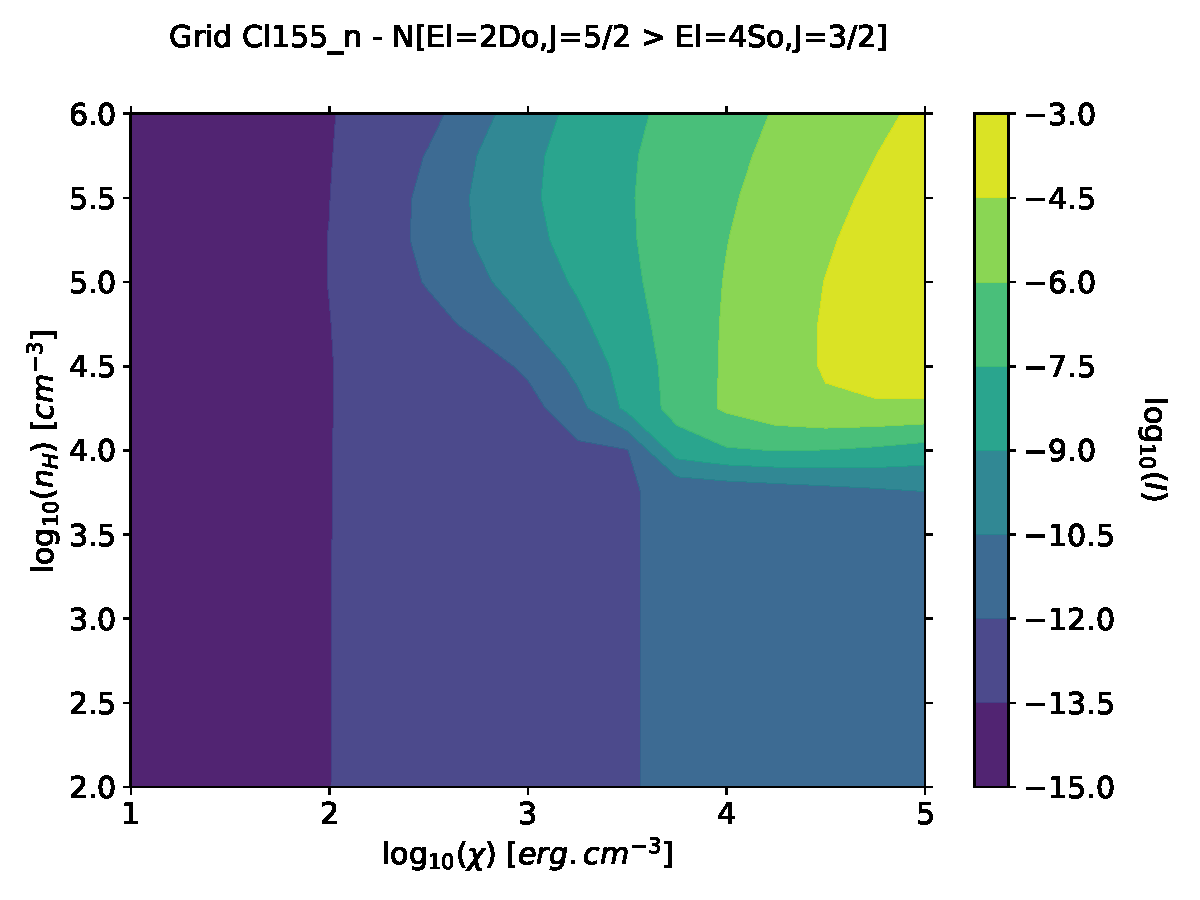
\includegraphics[trim = {0 0 0 1cm},clip,width=1\textwidth]{figure/Cl/gridModelEmiss/mapI_N.pdf}
        \caption{Emissivité de la raie [N] $5200.257 \mathrm{A}$ d'une grille de modèle avec Chlore.}
    \end{subfigure}
    ~ 
    \begin{subfigure}[t]{0.49\textwidth} % "0.49" donne ici la largeur de l'image
        \centering 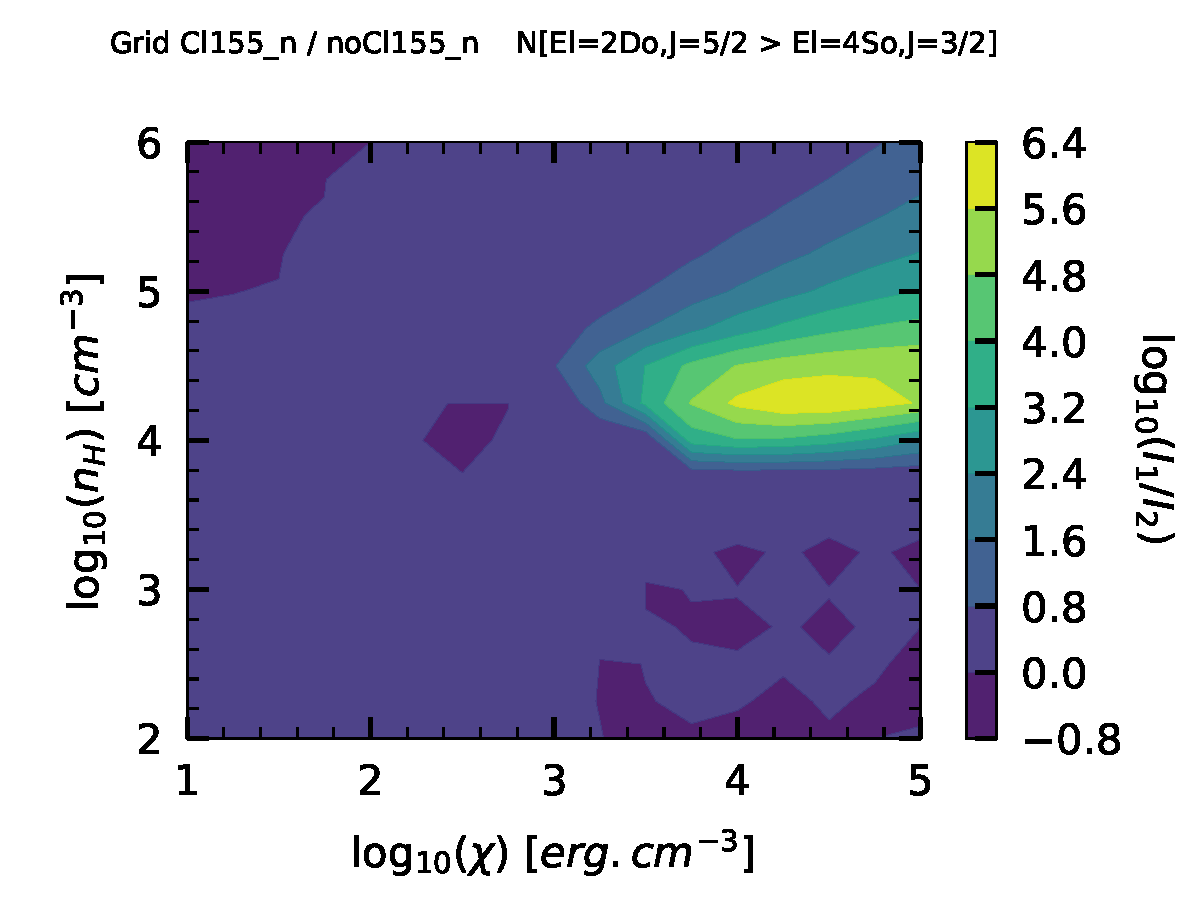
\includegraphics[trim = {0 0 0 1cm},clip,width=1\textwidth]{figure/Cl/gridModelEmiss/map_Cl155_n_noCl155_nI_N.pdf}
        \caption{Rapport des émissivités dans le cas avec ou sans chlore des grilles de modèles}
    \end{subfigure}
    
    \caption{}
    \label{fig:Cl:gridModelEmiss:N}
\end{figure}


%%%%%%%%%%%%%%%%%%%%%%%%%%%%%%%%%%%%%%%%%%%%%%%%%%%%%%%%%%%%%%%%%%%%%%%%%%%%%%%%%%%%%%%%%%%%%%%

\subsection{Bonus}
\subsubsection{Chauffage à l'entrée du nuage moléculaire}

Il arrive qu'en entrée du nuage moléculaire, la température du gaz augmente de manière irrégulière. Dans cette région, l'effet photoélectrique devient encore plus efficace en raison de l'augmentation de la fraction électronique du nuage. La recombinaison sur les grains est d'autant plus rapide que la fraction électronique est grande. 

% Dans cette région du nuage, le $\mathrm{H}_2$ se forme principalement sut les grains mais aussi par l'association radiative de l'hydrogène :

% \begin{equation}
%     \begin{array}{lccccclr}
%       \mathrm{H}  & + & e^- & \rightarrow & \mathrm{H}^{-} & + & h\nu &  \\
%     \end{array}
% \end{equation}

% avec un coefficient de réaction $k(T) = 1.9\, 10^{-16} \big(\frac{T}{100}\big)^{0.67} \, \mathrm{cm}^3\mathrm{s}^{-1}$, suivi d'un détachement associatif :

% \begin{equation}
%     \begin{array}{lcccccclr}
%       \mathrm{H}  & + &  \mathrm{H}^- & \rightarrow & \mathrm{H}_2 & + & e^- & + & KE\\
%     \end{array}
% \end{equation}

% ou $\xi = 2.4\, 10^{-7} G_0 \, \mathrm{s}^{-1}$. 

On a remarqué que pour une PDR avec $n_\mathrm{H} = 10^{3.5} \, \mathrm{cm}^{-3}$ et $\chi = 10^{4.5}$, la température augmentait en pic avant le nuage moléculaire (figure \ref{fig:H2:recomb:profilH}). On cherche à comprendre quel phénomène est à l'origine de l'augmentation de la température ? Pourquoi le taux de H2 diminue t il en même temps ? Pourquoi prendre en compte les nouveaux taux de collisions accentue ce phénomène ? Qu'est ce qui provoque la monté ? Pourquoi ça s'arrête : lorsque la température du gaz est trop élevé, les états ro-vibrationelles de H2 sont remplis et se desexcitent en émettant des photons. On le voit sur la figure \ref{fig:H2:recomb:profilH} ou le chauffage par H2 cessent de chauffer.

\begin{figure}[!htbp]
    \centering
    \begin{subfigure}[t]{0.49\textwidth} % "0.49" donne ici la largeur de l'image
        \centering 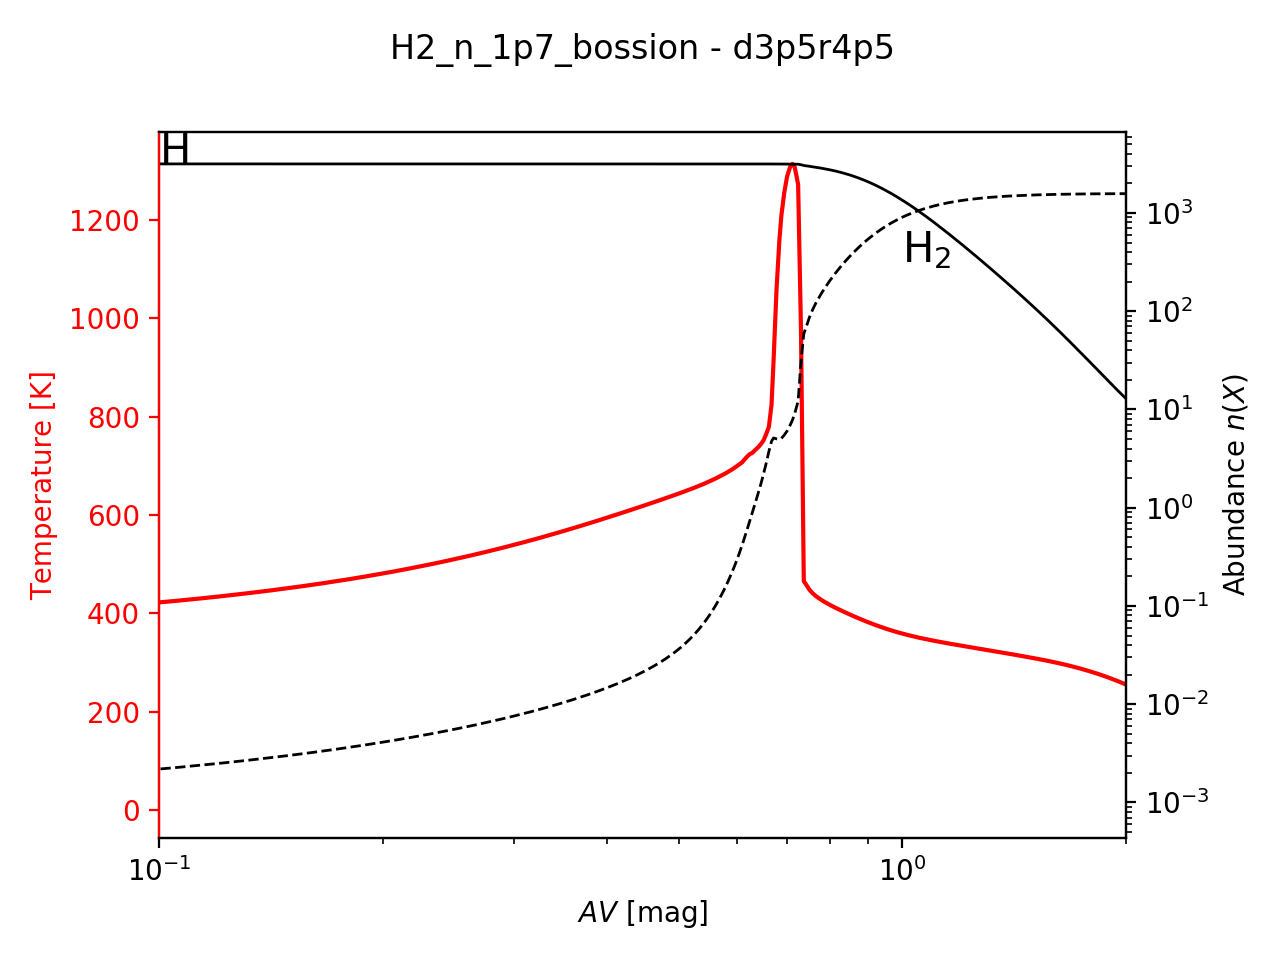
\includegraphics[trim = {0 0 0 1cm},clip,width=1\textwidth]{figure/H2/rec_elec/H2_n_1p7_bossion_d3p5r4p5_H.png}
        \caption{}
    \end{subfigure}
    ~ 
    \begin{subfigure}[t]{0.49\textwidth} % "0.49" donne ici la largeur de l'image
        \centering 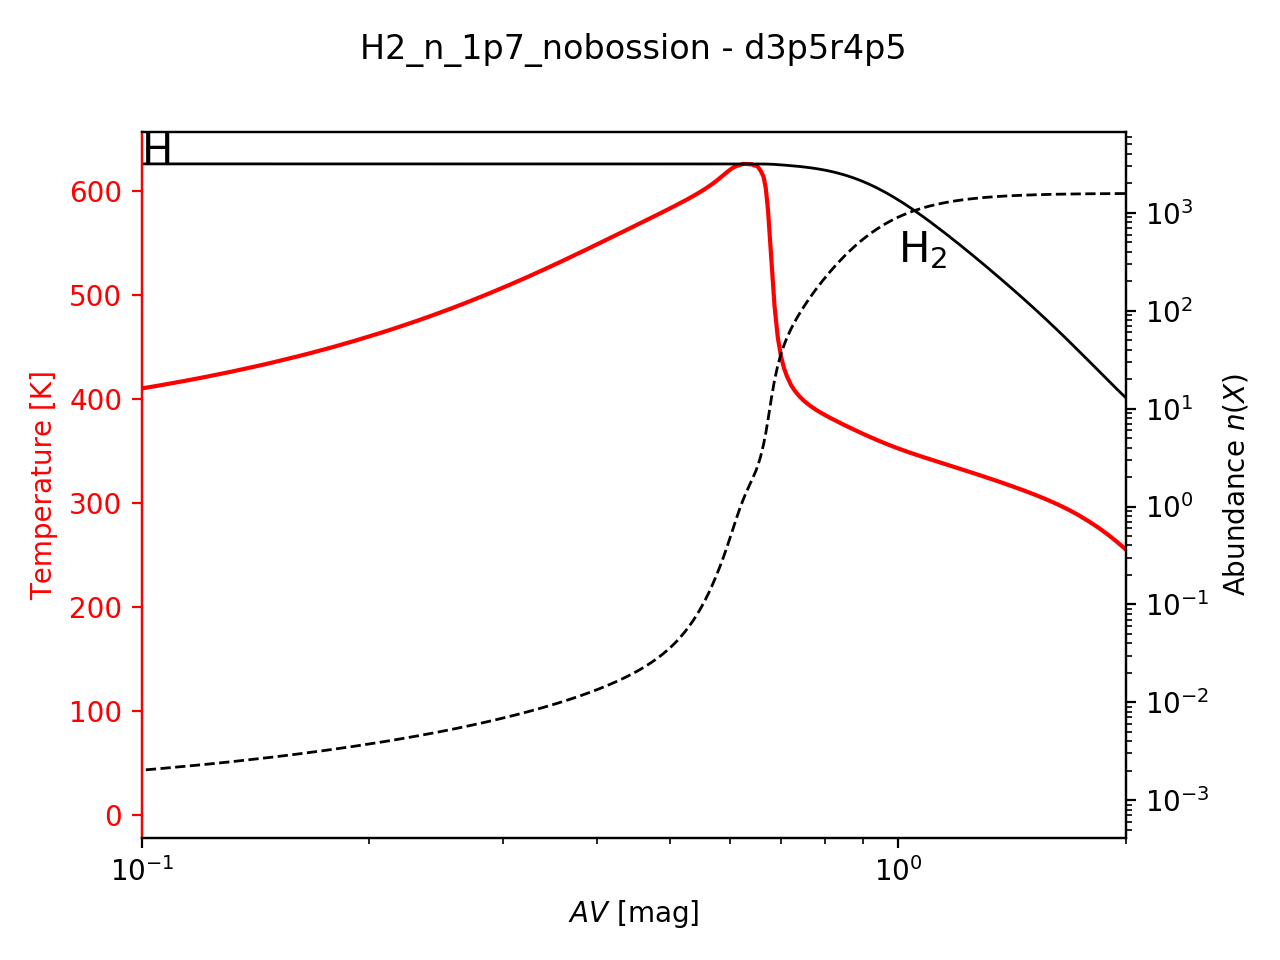
\includegraphics[trim = {0 0 0 1cm},clip,width=1\textwidth]{figure/H2/rec_elec/H2_n_1p7_nobossion_d3p5r4p5_H.png}
        \caption{}
    \end{subfigure}
    
    \caption{Profil de température et de densités de $\mathrm{H}$ et $\mathrm{H}_2$. A l'entrée du nuage la température augmente accompagné d'une légère diminution de la densité de $\mathrm{H}_2$. Cet effet est accentué sur (a) qui prend en compte les nouveaux taux de collision de $\mathrm{H}_2$. }
    \label{fig:H2:recomb:profilH}
\end{figure}
    
\begin{figure}[!htbp]
    \centering
    \begin{subfigure}[t]{0.49\textwidth} % "0.49" donne ici la largeur de l'image
        \centering 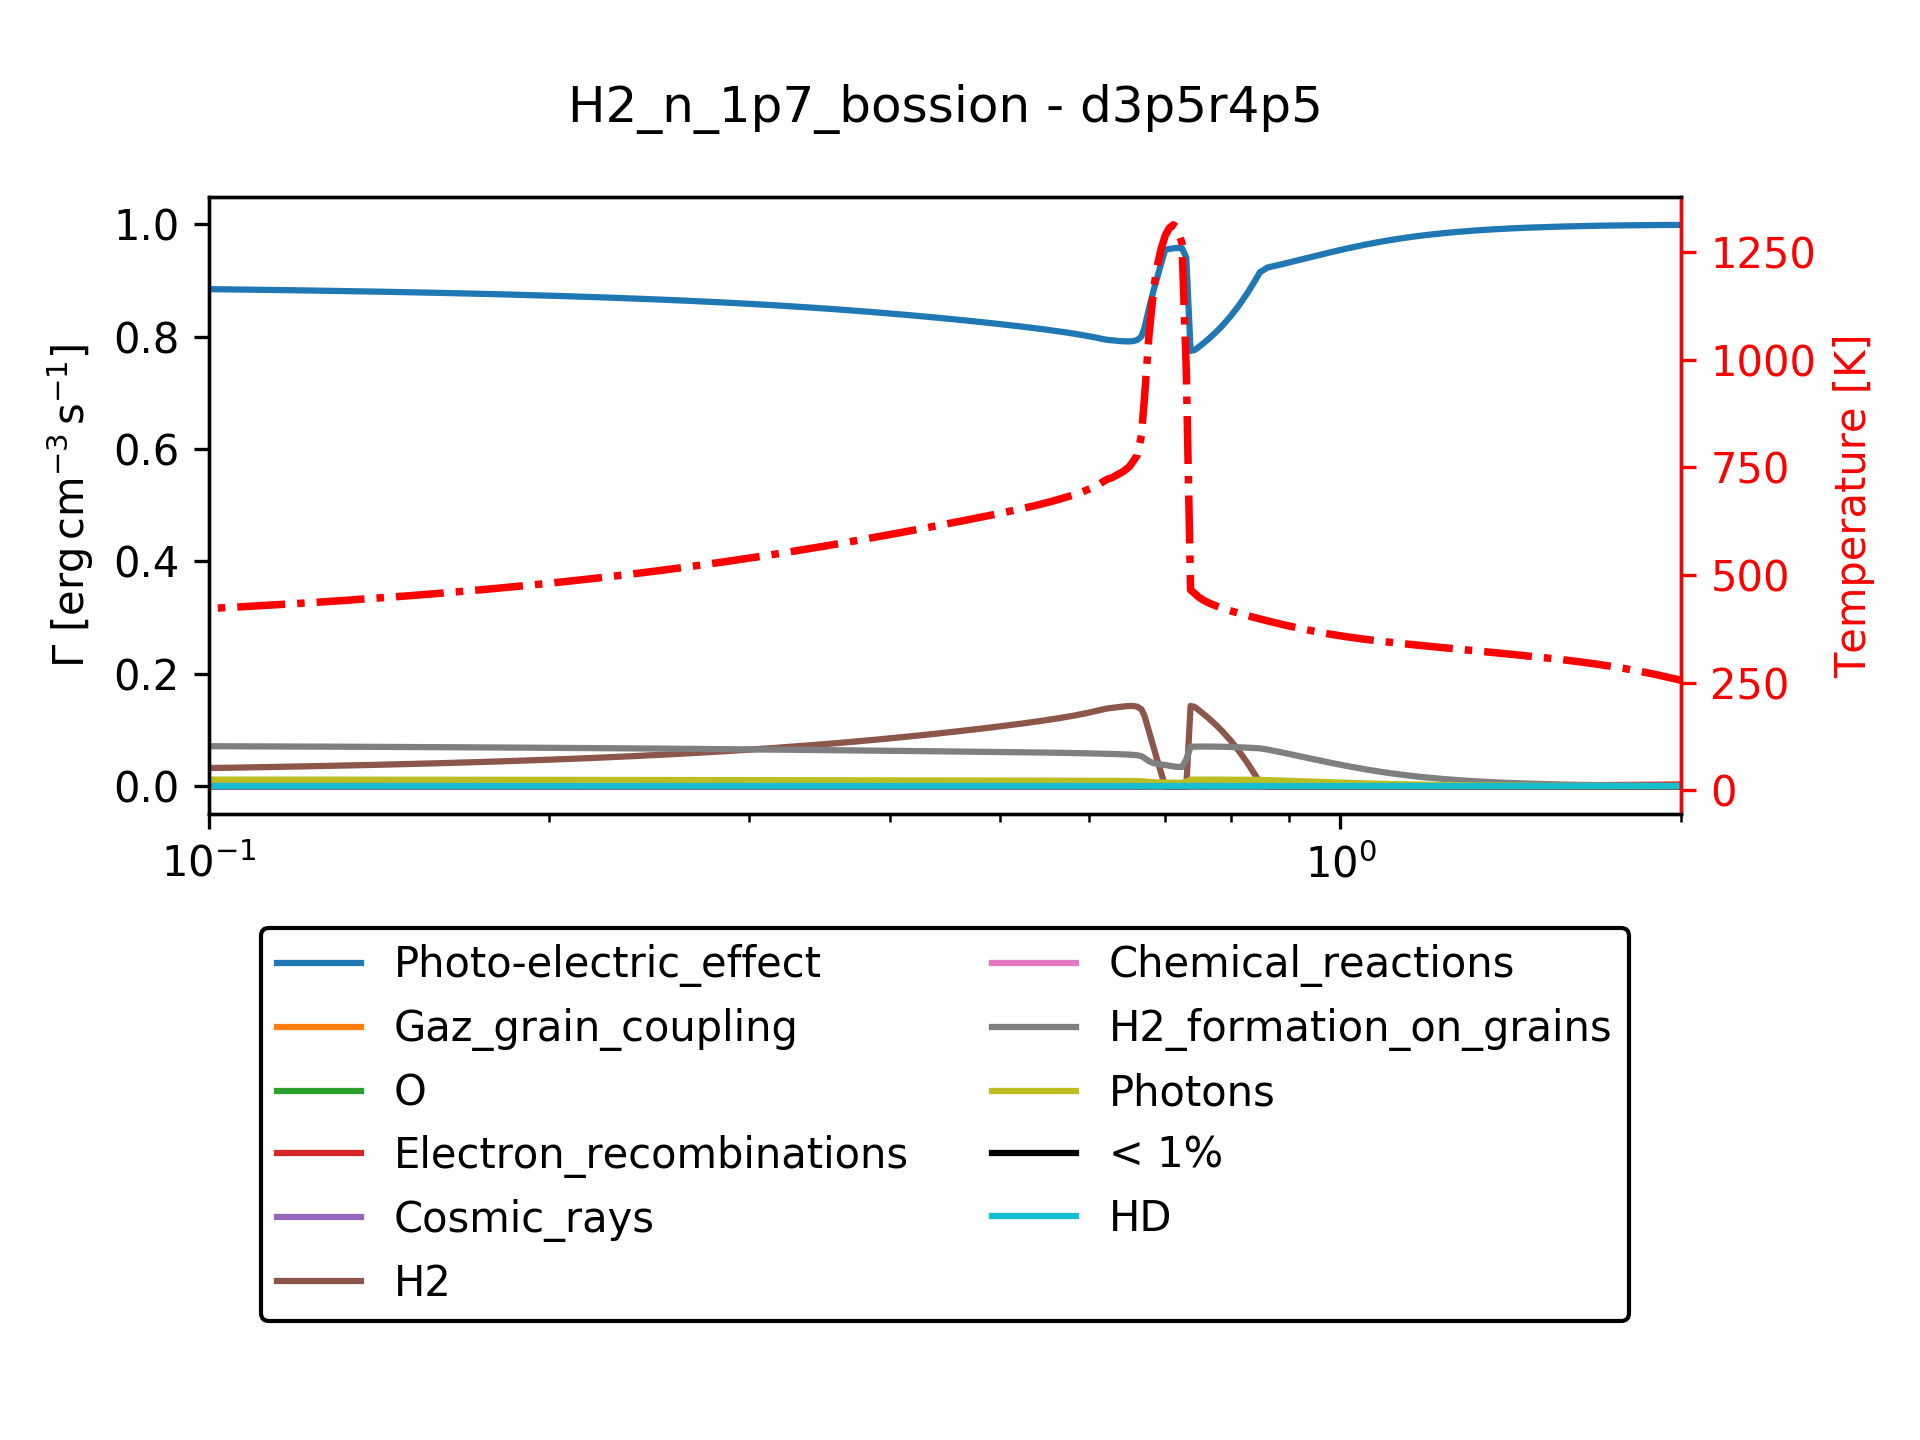
\includegraphics[trim = {0 0 0 1cm},clip,width=1\textwidth]{figure/H2/rec_elec/H2_n_1p7_bossion_d3p5r4p5hc_rheat.png}
        \caption{Avec les nouveaux taux de collisions}
    \end{subfigure}
    ~ 
    \begin{subfigure}[t]{0.49\textwidth} % "0.49" donne ici la largeur de l'image
        \centering 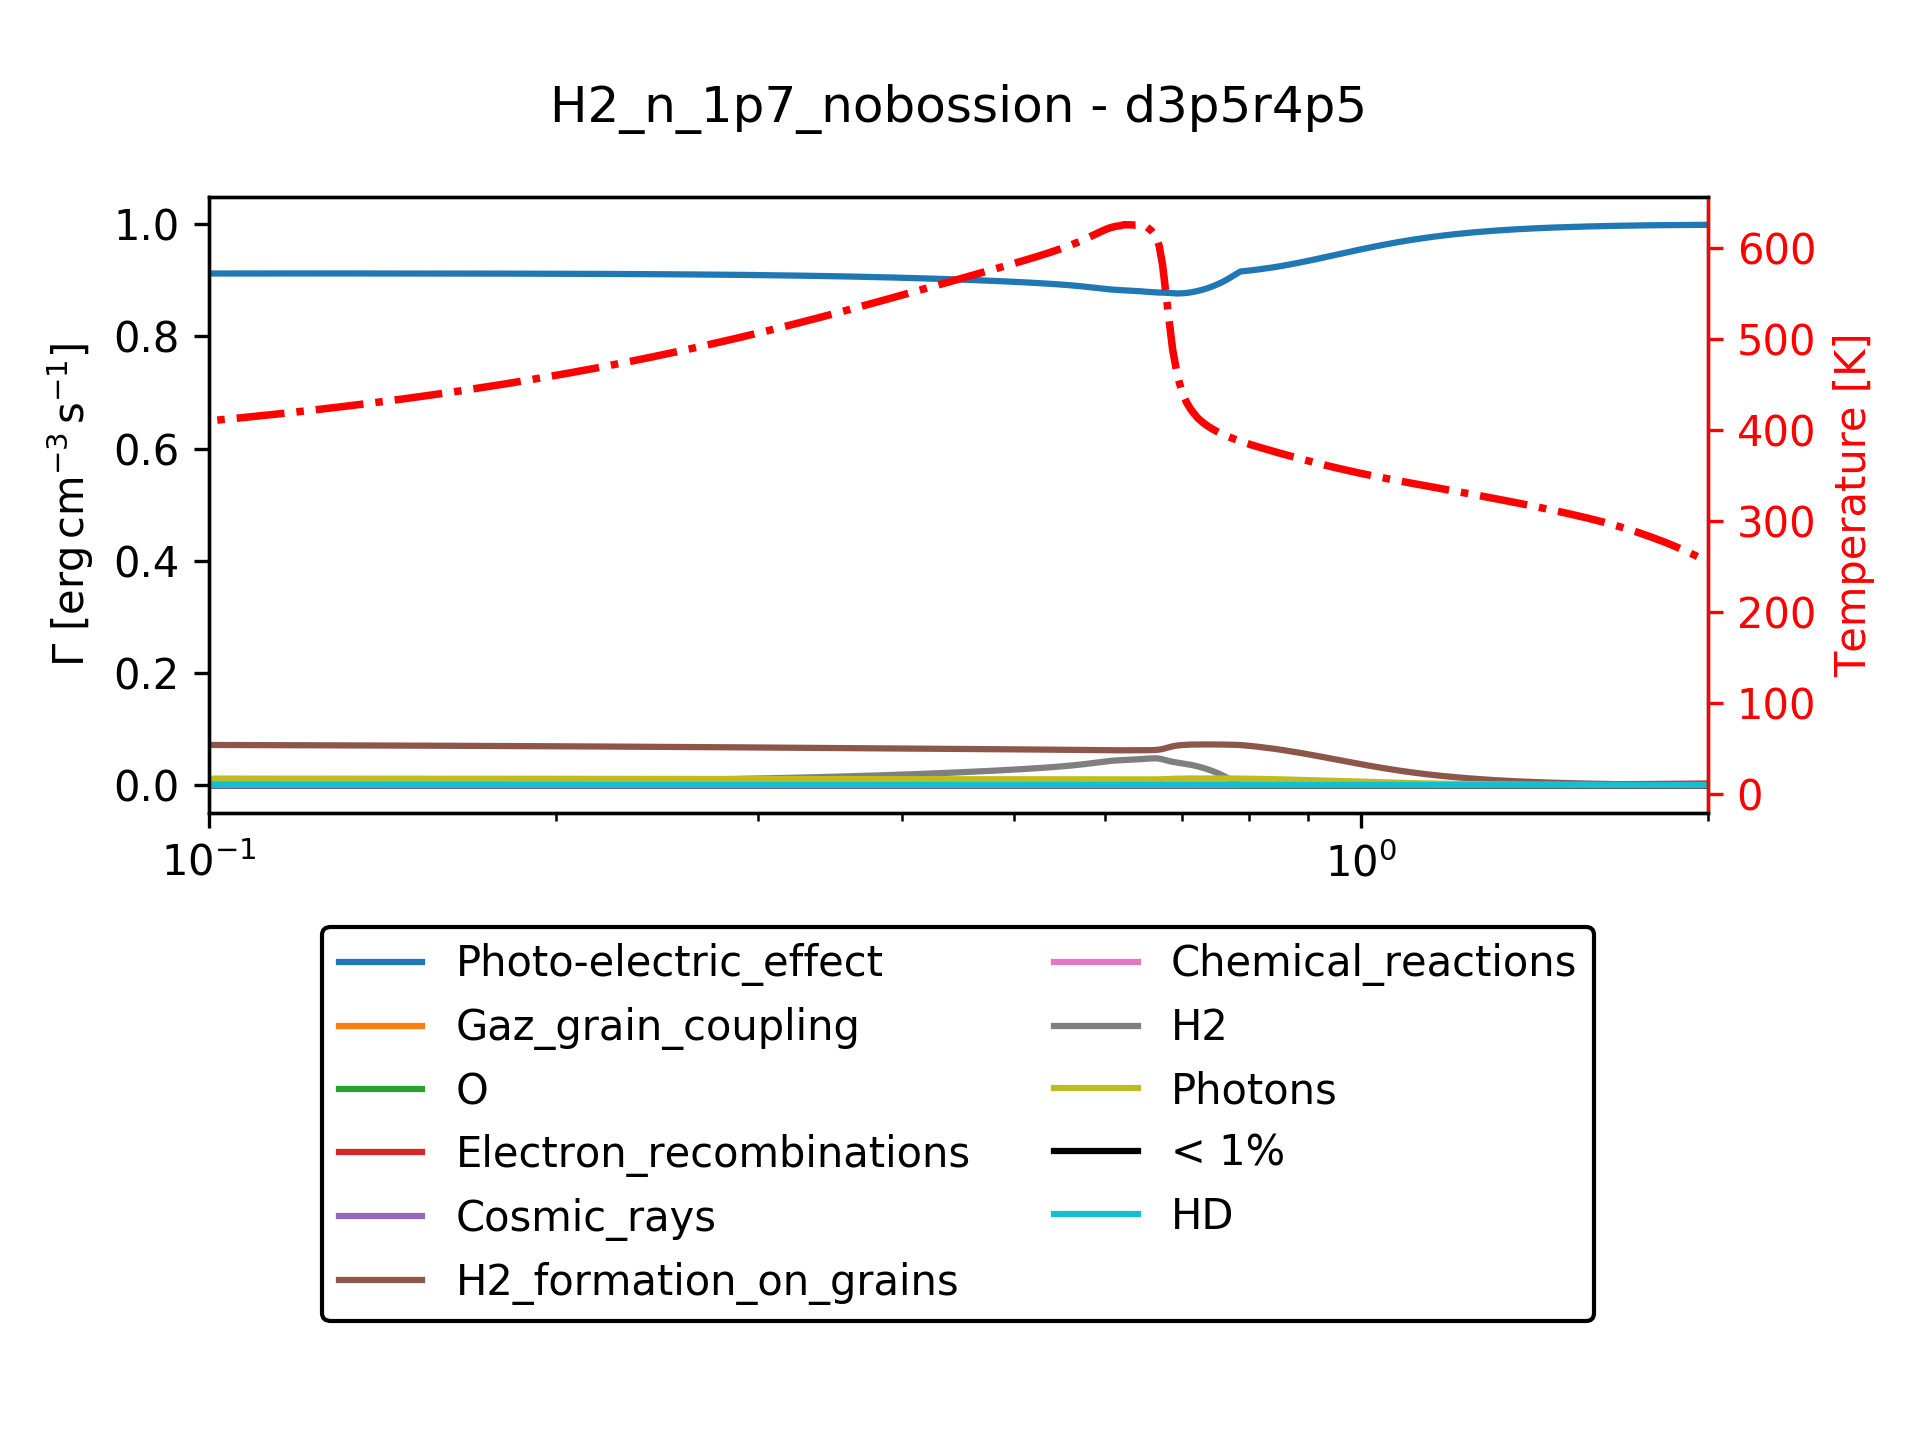
\includegraphics[trim = {0 0 0 1cm},clip,width=1\textwidth]{figure/H2/rec_elec/H2_n_1p7_nobossion_d3p5r4p5hc_rheat.png}
        \caption{Sans les nouveaux taux de collisions}
    \end{subfigure}
    \caption{Taux de chauffage (en relatif) en fonction de l'extinction. Dans les deux situations le chauffage par effet photo-électrique est le phénomène dominant pendant l'irrégularité tandis que le chauffage par $\mathrm{H}_2$ devient refroidisseur. Cet effet est accentué si l'on prend en compte les nouveaux taux de collisions.}
    \label{fig:H2:recomb:profilH}
\end{figure}

On a tracé une figure comparant la température, la densité de molécules $\mathrm{H}_2$ et la densité d'électrons à l'entrée du nuage moléculaire (\ref{fig:recomb:comp}). Ce pic abrupte est du à la prise en compte des taux de collisions. On observe aussi une monté (moindre) avec Janev et Glover sans les nouveaux taux (modèles densités constantes).

\begin{figure}
    \centering
    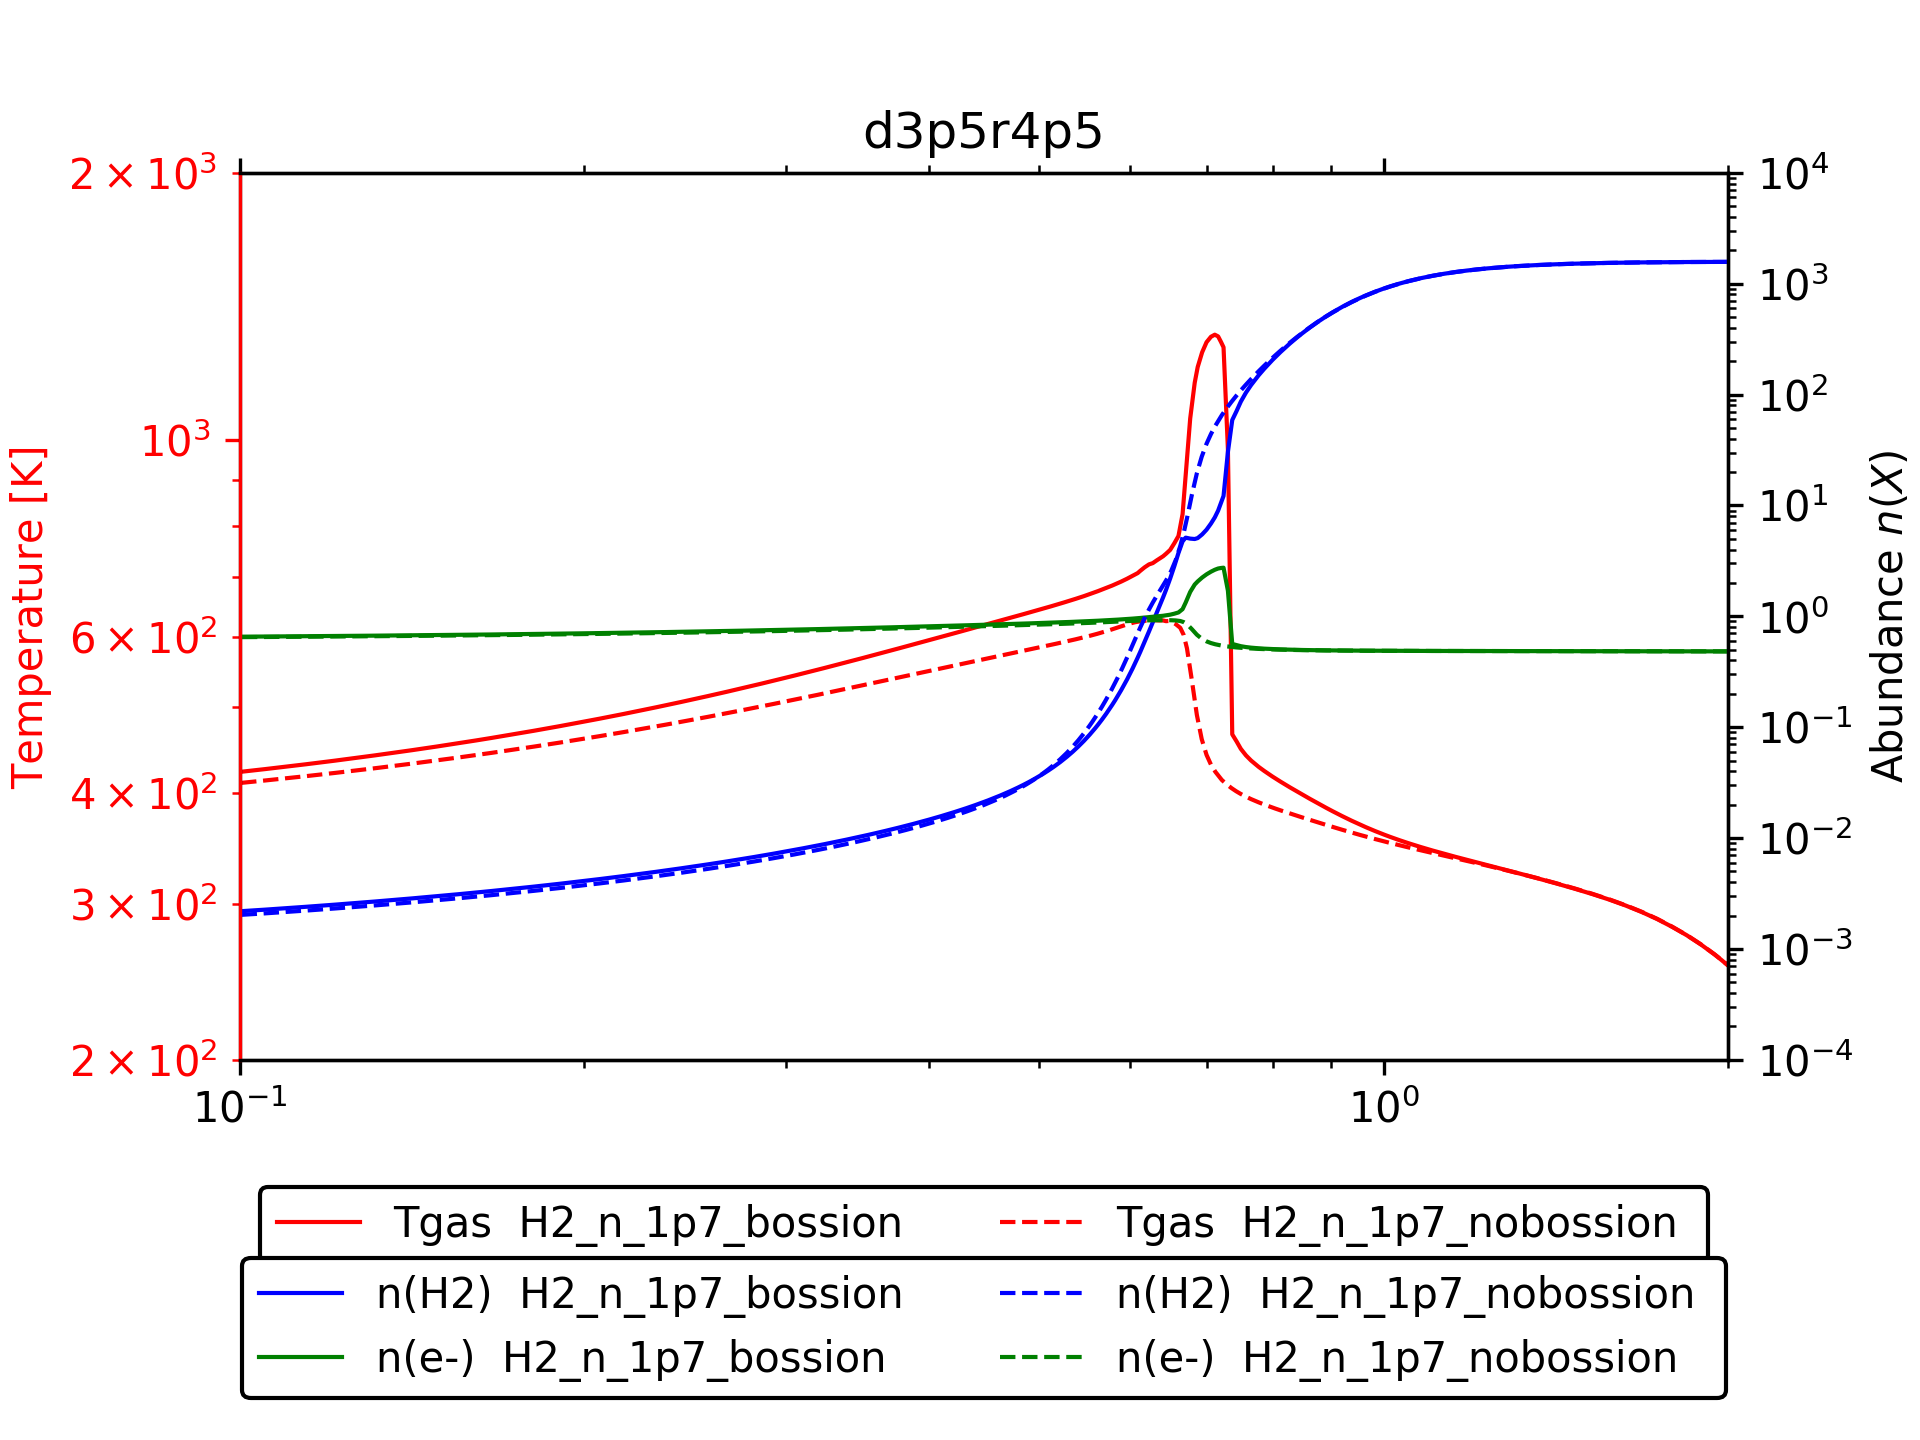
\includegraphics[trim = {0 0 0 0},clip,width=0.6\textwidth]{figure/H2/rec_elec/nT_H2_H2_n_1p7_bossion_H2_n_1p7_nobossion.png}
    \caption{}
    \label{fig:recomb:comp}
\end{figure}